% Outras Opções:
%   * openright  -- Força início de capítulos em páginas ímpares (padrão da
%                   biblioteca)
%   * oneside    -- Desliga frente-e-verso
%   * nominatalocal -- Lê os dados da nominata do arquivo nominatalocal.def
\documentclass[ppgc,diss,english,openright]{iiufrgs}

\usepackage[utf8]{inputenc}
\usepackage[alf,abnt-emphasize=bf]{abntex2cite}	% pacote para usar citações abnt

\usepackage{lmodern}
\usepackage{amsmath}
\usepackage{amsthm}
\usepackage{enumitem}
\usepackage{listings}
\usepackage{xcolor}
\usepackage{amsfonts}
\usepackage{newtxtext,newtxmath}
\usepackage{semantic}
\usepackage{float}
\usepackage{mdframed}
\usepackage{stmaryrd}
\usepackage{multicol}
\usepackage{graphicx}
\usepackage{todonotes}
\usepackage{mathtools}
\usepackage{etoolbox}
\usepackage[normalem]{ulem}
\usepackage{fontawesome}

\usepackage{times}
\usepackage{palatino}
\usepackage[all,knot,arc,import,poly]{xy}

\usepackage{tikz,tkz-euclide}
\usetikzlibrary{backgrounds,calc,shapes,shapes.geometric}
%\usepackage{subfig}
\usepackage{caption}
\usepackage{subcaption}
\captionsetup[subfigure]{justification=centering}

\usepackage{pdfpages}

\usepackage{wasysym}
\usepackage{minted}

%For todo notes, remove in final version
\setlength{\marginparwidth}{2cm}
\newcommand{\tinytodo}[2][]
{\todo[caption={#2}, size=\footnotesize, #1]{\renewcommand{\baselinestretch}{0.5}\selectfont#2\par}}

\newcommand{\critical}[1]{\todo[color=red]{\textbf{Critical:} #1}}
\newcommand{\important}[1]{\textcolor{red}{\textbf{\texttt{#1}}}}
%\newcommand{\newadd}[1]{\uline{#1}}
\newcommand{\newadd}[1]{#1}

\theoremstyle{plain}
\newtheorem{thm}{Theorem}[chapter]

\theoremstyle{definition}
\newtheorem{definition}[thm]{Definition}
\newtheorem{example}[thm]{Example}
\newtheorem{assumption}[thm]{Assumption}
\newtheorem*{remark}{Remark}
\newtheorem*{notation}{Notation}
\AtEndEnvironment{definition}{\hfill\qedsymbol}%put \null before \hfill?
\AtEndEnvironment{assumption}{\hfill\qedsymbol}
\AtEndEnvironment{remark}{\hfill\qedsymbol}
\AtEndEnvironment{notation}{\hfill\qedsymbol}
\AtEndEnvironment{example}{\hfill$\blacksquare$}

\def\changemargin#1#2{\list{}{\rightmargin#2\leftmargin#1}\item[]}
\let\endchangemargin=\endlist

\newenvironment{intuition}{\begin{changemargin}{1cm}{1cm}}{\end{changemargin}}

%% Diagram commands
\newcommand{\diagram}[1]{\centerline{\xymatrix{#1}}}
\newcommand{\parens}[1]{\left(#1\right)}
\newcommand{\morph}[3]{\mbox{${#1} : {#2} \rightarrow {#3}$}}

%% Graph Grammars constructions
\newcommand{\graphrule}{\mbox{$p = \left(L \xleftarrow{l} K \xrightarrow{r} R\right)$}}
\newcommand{\ruleone}{\mbox{$p_1 = \left(L_1 \leftarrow K_1 \rightarrow R_1\right)$}}
\newcommand{\ruletwo}{\mbox{$p_2 = \left(L_2 \leftarrow K_2 \rightarrow R_2\right)$}}
\newcommand{\inversegraphrule}{\mbox{$p^{-1} = \left(R \xleftarrow{r} K \xrightarrow{l} L\right)$}}
\newcommand{\lefthand}{\mbox{$l : K \rightarrow L$}}
\newcommand{\righthand}{\mbox{$r : K \rightarrow R$}}
\newcommand{\nac}{\mbox{$n : L \rightarrow N$}}
\newcommand{\nacone}{\mbox{$n_1 : L_1 \rightarrow N_1$}}
\newcommand{\nactwo}{\mbox{$n_2 : L_2 \rightarrow N_2$}}
\newcommand{\rightnac}{\mbox{$n : R \rightarrow N$}}
\newcommand{\match}{\mbox{$m : L \rightarrow G$}}
\newcommand{\comatch}{\mbox{$m' : R \rightarrow H$}}
\newcommand{\rulesequence}{\mbox{$p_0,\ldots,p_{n-1},p_n$}}
\newcommand{\graphGrammar}{\mbox{$GG = \left(TG,I,P\right)$}}

%% Doubly-typed Graph Gramars constructions
\newcommand{\doublyTypedGraph}{\mbox{$G^{TG^{T}}$}}
\newcommand{\doublyTypedRule}{\mbox{$p^{TG^T} = \left(L^{TG^T} \leftarrow K^{TG^T} \rightarrow R^{TG^T}\right)$}}
\newcommand{\inverseDoublyTypedRule}{\mbox{$\parens{p^{TG^T}}^{-1} = \left(R^{TG^T} \leftarrow K^{TG^T} \rightarrow L^{TG^T}\right)$}}
\newcommand{\doublyTypedGraphGrammar}{\mbox{$GG = \left(TG^T, I^{TG^T},P \right)$}}
\newcommand{\doublyTypedGraphGrammarCore}{\mbox{\ensuremath{GG = \left(C^T, I^{C^T},P \right)}}}
\newcommand{\occurrenceGrammar}{\mbox{\ensuremath{OGG = \left(C^T, I^{C^T},A \right)}}}
\newcommand{\coreGraph}{\ensuremath{C^T}}
\newcommand{\action}{\mbox{$a = \left(L_a \xleftarrow{l} K_a \xrightarrow{r} R_a, L_a \xrightarrow{n_i} [N_i]\right)$}}
\newcommand{\initialGraph}{\mbox{\ensuremath{I^{\coreGraph}}}}

%% Category Constructions
\newcommand{\cat}[1]{\mbox{\ensuremath{\mathbf{#1}}}}
\newcommand{\typedGraphCategory}{\cat{TGraph_T}}
\newcommand{\doublyTypedGraphCategory}{\cat{DTGraph_{TG^T}}}

\newcommand{\code}[1]{\texttt{#1}}
\newcommand{\hide}[1]{}

\newcounter{doubly-typed-grammar-counter}
\addtocounter{doubly-typed-grammar-counter}{0}


% avoid LaTeX Font Warning: Font shape `U/stmry/b/n' undefined
\SetSymbolFont{stmry}{bold}{U}{stmry}{m}{n}

\title{Occurrence Graph Grammars with Negative Application Conditions}
\author{Santos Bezerra}{Jonas}
\advisor[Prof$^a$.]{Ribeiro}{Leila}
%\date{maio}{2001}
\location{Porto Alegre}{RS}

% itens individuais da nominata podem ser redefinidos com os comandos
% abaixo:
% \renewcommand{\nominataReit}{Prof\textsuperscript{a}.~Wrana Maria Panizzi}
% \renewcommand{\nominataReitname}{Reitora}
% \renewcommand{\nominataPRE}{Prof.~Jos{\'e} Carlos Ferraz Hennemann}
% \renewcommand{\nominataPREname}{Pr{\'o}-Reitor de Ensino}
% \renewcommand{\nominataPRAPG}{Prof\textsuperscript{a}.~Joc{\'e}lia Grazia}
% \renewcommand{\nominataPRAPGname}{Pr{\'o}-Reitora Adjunta de P{\'o}s-Gradua{\c{c}}{\~a}o}
% \renewcommand{\nominataDir}{Prof.~Philippe Olivier Alexandre Navaux}
% \renewcommand{\nominataDirname}{Diretor do Instituto de Inform{\'a}tica}
% \renewcommand{\nominataCoord}{Prof.~Carlos Alberto Heuser}
% \renewcommand{\nominataCoordname}{Coordenador do PPGC}
% \renewcommand{\nominataBibchefe}{Beatriz Regina Bastos Haro}
% \renewcommand{\nominataBibchefename}{Bibliotec{\'a}ria-chefe do Instituto de Inform{\'a}tica}
% \renewcommand{\nominataChefeINA}{Prof.~Jos{\'e} Valdeni de Lima}
% \renewcommand{\nominataChefeINAname}{Chefe do \deptINA}
% \renewcommand{\nominataChefeINT}{Prof.~Leila Ribeiro}
% \renewcommand{\nominataChefeINTname}{Chefe do \deptINT}

\keyword{Graph Grammars}
\keyword{Occurrence Graph Grammars}
\keyword{Negative Aplication Conditions}
\keyword{Semantics}

\newcommand{\pu}{processing unit}
\newcommand{\Pu}{Processing unit}
\newcommand{\pus}{processing units}
\newcommand{\Pus}{Processing units}
\newcommand{\envid}{env_{id}}

\definecolor{kwcolor}{rgb}{0,0.5,0}
\definecolor{bgcolor}{rgb}{0.98, 0.98, 0.98}
\definecolor{numbercolor}{rgb}{0.1,0.1,0.1}

\lstset{
  keywordstyle=\bfseries\underbar,
  stringstyle=\itshape,
  basicstyle=\small\ttfamily,
  frame=bt,
  framerule=1pt,
  numbers=left,
  numbersep=10pt,
  numberstyle=\scriptsize\color{numbercolor},
  backgroundcolor=\color{bgcolor},
  tabsize=2
}

\lstdefinelanguage{l1}
{keywords={let, letrec, in, if, then, else, end, unused}%
  sensitive=true,
  alsoletter={\$},
  comment=[l]{\#},
  string=[b]"
}

\lstdefinelanguage{acqua-ir}
{keywords={unused, EnvNew, EnvAdd, Call, unused}%
  sensitive=true,
  alsoletter={\$},
  comment=[l]{\#},
  string=[b]"
}

\graphicspath{ {images/} }
%\captionsetup[table]{skip=10pt}
\newmdenv[leftline=false,rightline=false]{openframe}



\captionsetup[figure]{position=below,labelfont=bf}
\captionsetup[subfigure]{position=bottom}
\sloppy
\begin{document}

\hide{ Template for code snippets
\begin{figure}[!ht]
\caption{Colimit Implementation}
\begin{minted}[linenos=true, breaklines,fontsize=\small]{haskell}
\end{minted}
\label{fig:tests-colimit}
\end{figure}
}

\maketitle
\clearpage

% dedicatoria
\clearpage
\begin{flushright}
  \mbox{}\vfill
  {\sffamily\itshape
  ``Poste, kiam \^si pripensis la aferon,\\
  \^si opiniis ke tio ja estis mirinda,\\
  sed kiam \^gi okazis \^cio \^sajnis tute natura.''\\}
  --- \textsc{Alico en Mirlando}
\end{flushright}

% agradecimentos
\chapter*{Acknowledgement}
  I'm very happy with everything I've accomplished so far and although I still have a long way to go, I must thank some amazing people in my life without whom this path would be a lot harder, if not impossible.

  First of all, I would like to thank Prof. Leila Ribeiro for giving me the opportunity to work with her even without previously knowing me: You are such an inspiring advisor and working with you always made me feel like I can improve myself and push me to the next level. Working with you was, at the same time, very challenging and joyful. I also need to thank professors Rodrigo Machado, Érika Cota and Lúcio Duarte, for always being there for conversations and feedback about this work, you were really a great help.

  I owe a very special thank you to Calebe and Marília, for helping me settle in Porto Alegre when I knew nothing, nowhere and nobody here. You guys really made my life a lot easier.

  To Andrei, Guilherme, Leonardo and Ana, my colleagues and friends, it was both an honour and a pleasure to work and live with you. I will always cherish our memories together as some of my favourites. To all the guys from lab 202, Diego, Fabi, Marcelo, Marina, Marlo, Felipe Tanus, Michele, Felipe Grando, Jéssica e Pedro: we need to go out more. To my very first friends in Porto Alegre, Shauna and Maurício, thank you for all the good moments. 

  To my old friends, Wendell, Gabriel, Malu and Jéssica, who were always by my side despite the 3178km of distance, your constant contact and kindness helped me through a lot of critical moments. I love you guys.

  Ao meu irmão, Mateus, com quem eu sei que sempre posso contar e por quem eu sempre tentei dar o melhor de mim, de tal forma que ele tenha tanto orgulho de quem eu sou e da família que formamos: obrigado por me aceitar como eu sou.
  
  Finalmente, para mainha, Dona Necila... eu jamais poderei expressar suficientemente o quão a senhora foi importante em todas as minhas conquistas até agora. A senhora sempre foi a pessoa que mais admiro na vida, por toda sua luta, dedicação e sacrifícios para dar a mim e aos meus irmãos todas as oportunidades que a senhora não teve. Esse mestrado é tão seu quanto meu. Vou te amar pra sempre.

\begin{abstract}
    Graph Grammars are based on the application of rules that are able to modify graphs, as such, they provide a suitable formalism to model complex systems in an intuitive and precise manner, providing both a graphical, straightforward language and a solid formal background for systems analysis. Therefore, they have been used in a wide range of applications within Computer Science, specially in the field of Model-Driven Development.
    Particularly, the study of the Semantics of Graph Grammars, i.e. which graphs belong to the language of a grammar and which derivations are possible within the context of a grammar, provides a powerful framework for reasoning about the execution behaviour of systems modelled as Graph Grammars.
    There are several different ways of specifying the Semantics of Graph Grammars.
    One notable possibility is the use of Occurrence Graph Grammars, which encodes the Semantics in a structure that is also a Graph Grammar itself. Occurrence Graph Grammars were introduced in the nineties and used ever since, however the original definitions lack the inclusion of Negative Application Conditions, additional structures imposed over the rules of a grammar to better tune their possible applications according to the execution context.
    Given the important role Negative Application Conditions play in the modelling and analysis of complex systems as Graph Grammars nowadays, this thesis presents an extension of the framework of Occurrence Graph Grammars to include them. It also presents its implementation in Verigraph, a system specification and verification tool based on graph rewriting.
\end{abstract}

\begin{englishabstract}{Gramáticas de Grafos de Ocorrência com Condições Negativas de Aplicação}{Gramáticas de Grafos. Gramáticas de Grafos de Ocorrência. Condições Negativas de Aplicação. Semântica}
  Gramáticas de Grafos baseiam-se na aplicação de regras que modificam grafos, fornecendo assim um formalismo adequado para a modelagem de sistemas complexos de forma intuitiva e precisa, além de fornecer uma notação gráfica descomplicada e uma base formal sólida para a análise de sistemas. Dados tais atributos, essas gramáticas possuem uma ampla gama de aplicações dentro da Ciência da Computação, especialmente no campo do Desenvolvimento Orientado a Modelos. Particularmente, o estudo da semântica de
  Gramáticas de Grafos (isto é, quais grafos pertencem à linguagem da gramática e quais derivações são permitidas no contexto da gramática) provê uma poderosa ferramenta para compreender e analisar o comportamento de sistemas modelados como Gramáticas de Grafos. Existem diversas formas de especificar a semântica de Gramáticas de Grafos, uma delas é o uso de Gramáticas de Grafos de Ocorrência que codificam tal semântica em estruturas que também são, por sua vez, Gramáticas de Grafos. Gramáticas de
  Grafos de Ocorrência foram introduzidas nos anos noventa e utilizadas desde então, porém as definições originais não incluem o uso de Condições Negativas de Aplicação, estruturas adicionais anexadas às regras de uma gramática para refinar as possíveis aplicações das regras em determinados contextos. Dada a atual importância das Condições Negativas de Aplicação na modelagem de sistemas complexos, essa dissertação propõe uma extensão da teoria das Gramáticas de Grafos de Ocorrência de forma a
  incluí-las, além de apresentar a implementação desta teoria no Verigraph, uma ferramenta de especificação e verificação de sistemas baseada em reescrita de grafos.
\end{englishabstract}


\begin{listofabbrv}{SPMD}
   \item[DPO] Double Pushout
   \item[GG] Graph Grammar
   \item[GTS] Graph Transformation System
   \item[GUI] Graphical User Interface
   \item[NAC] Negative Application Condition
%   \item[NC] Negative Atomic Constraint
   \item[OGG] Occurrence Graph Grammar
%   \item[PB] Pullback
%   \item[PC] Positive Atomic Constraint
   \item[PO] Pushout
   \item[SPO] Single Pushout
\end{listofabbrv}

%  \begin{listofsymbols}{$\alpha\beta\pi\omega$}
%         \item[$\leftarrow$] Morphism
%  \end{listofsymbols}

\listoffigures
\tableofcontents

\chapter{Introduction}

Graph grammars are a suitable formalism to model complex systems in an intuitive and precise manner, providing both a graphical language and a solid formal background for systems analysis. In this framework, system states are modelled as graphs, while transitions between different states are modelled as graph transformation rules~\cite{Ehrig2006}. A graph transformation rule generically has the form $L \xRightarrow{p} R$, where there is at least one left side graph $L$ containing a pattern to be found (a match) in order for the rule to be applied over an instance graph and a right side graph $R$ corresponding to the effect of applying such a rule. Moreover, there are also additional structures that may be used as complements of rules to better tune which kinds of matches are acceptable to perform a transformation, for instance: Graph Constraints, Negative Application Conditions (NACs) and Nested Application Conditions, to cite some of the most commonly used.

There exist several approaches that might not only change the exact format of a rule, but also define different ways a rule can be applied over a given match. Only considering the domain of Category Theory there is already a handful of different approaches to graph grammars: the Single Pushout (SPO), Double Pushout (DPO), Sesqui-Pushout (SqPO), AGREE, among others. Each approach has its own advantages/disadvantages regarding the kinds of  ``operations'' they allow or forbid in the system under modelling. 
In spite of that, whichever approach is used, they all provide a way to describe the behaviour of the system together with means to analyse several properties about this behaviour, such as termination, concurrency and reachable states. Among the several analysis techniques provided by graph grammars, we have:

\begin{itemize}
  \item Critical Pair Analysis and Critical Sequence Analysis: critical pair analysis allows us to verify which rules conflict with (i.e. prohibit) the application of another and why; critical sequence analysis, which rules depend on the execution of others to be applied and why~\cite{Lambers2008a}; such analyses provide insights about the possible execution flows of the system.
  \item Calculation of Concurrent Rules: a concurrent rule summarizes in one rule the combined results of applying several different rules. In other words, it represents the combination of several different rules which can be then applied as a ``one step'' transformation rule~\cite{Lambers2008,BezerraETMF2016}.
  \item State Space Exploration and Model Checking: permits to verify, in an exhaustive fashion, whether the (graph grammar) model of a system satisfies a given specification and to prove the satisfaction of its properties~\cite{Rensink2004}.
  \item Unfolding, Graph Processes, Occurrence Graph Grammars and Canonical Derivations: they are all different means to provide the semantics of Graph Grammars, allowing us to check which graphs belong to the language of a grammar and/or which concrete derivations are possible within that grammar~\cite{Corradini1996,Ribeiro1996}.
\end{itemize}

Graph grammars have found a wide range of applications within Computer Science, specially in the field of model-driven software development, where the transformation of visual models is a vital part of the process, therefore a natural application of graph grammars~\cite{Rozenberg1997}.
As evidence of such suitability, several non-trivial systems have been modelled and studied under the optics of graph grammars, such as telephone communications~\cite{Ribeiro1996}, elevator control~\cite{Lambers2010}, railroad control~\cite{Pennemann2009} and integration of service-oriented systems~\cite{Giese2015}.
Furthermore, there are a number of software tools to support the use of graph grammars, such as AGG, a tool environment for algebraic graph transformation~\cite{Taentzer2000}; Groove, a tool for state space generation~\cite{Rensink2004} and Verigraph, a software specification and verification tool based on graph rewriting~\cite{verigraph}.

Besides its powerful applications, the use of graph grammars as a framework for modelling systems provides us with a great advantage over other formalisms: it makes it possible for non-specialists in the field to generate graph grammar models of a system and then benefit from the rigorous analyses it offers without the need for a deep understanding of its underlying theory. For example, ~\cite{Junior2015,BezerraWEIT2016,Cota2017} explain how to generate graph grammars from a set of textual requirement documents such as use cases, functional specifications and other kinds of guidelines by means of a systematic methodology. They also present guidance towards using different graph grammars analysis techniques in order to improve and verify these documents and, consequently, the systems they describe.

The field of Graph Grammars is a very active one, and researches continuously develop new ideas, such as new graph transformation approaches (e.g. Sesqui-Pushout, AGREE), analysis techniques (e.g. Essential Critical Pairs), tools (e.g. Verigraph) and ways to apply them.
Additionally, we may also benefit from the combination of already existing techniques, which is what we do in this thesis.
In our work, we combine two concepts of the Graph Grammar Theory: Occurrence Graph Grammars, defined for the SPO and DPO approaches by~\cite{Ribeiro1996, Corradini1996}, with Negative Application Conditions, defined generically by~\cite{Habel1996}, which has not been done so far.

Occurrence Graph Grammars provides a semantics for Graph Grammars encoded in structures that are also Graph Grammars themselves. 
This semantics, which tells us which graphs are part of the grammar language and which graph transformations are possible within the context of the original grammar, may be used for the analysis of the system execution in a summarized fashion and also be used for practical applications, such as test cases generation, without the necessity to use a supplementary structure or formalism.

Negative Application Conditions (NACs) are extensions of rules encoding patterns that, if found in the match of a rule, forbids the transformation. In theory, they do not give any more expressive power to a graph grammar than using only rules without them~\cite{Habel1996}. In practice, they allow the modelling of systems in a much more concise and compact manner. Therefore they became really necessary in the modelling of complex, real-like systems~\cite{Corradini2013, Corradini2014}.

Our work here consists of the development of an extension for the framework of Occurrence Graph Grammars in the Double Pushout (DPO) approach in order to incorporate Negative Application Conditions, alongside with the implementation of this extension in the Verigraph system, a generic graph rewriting system based on Category Theory and written in Haskell. This implementation choice makes possible for the source code of the tool to be close to the theory domain as well as allowing other researches to implement new approaches or different models of graphs while benefiting from the already implemented techniques (as long as they conform to the categorial constructions).

%We believe that the use of graph grammars as a model for the generation of test cases and oracles may improve the reliability of the testing activity by using the solid formal semantics of the formalism, while requiring little theoretical expertise from the user. The main objective of this thesis can be summarized as follows:

%\begin{intuition}
%  \center{\textit{Given the graph grammar model of a software system, how can a set of relevant test cases and oracles be generated for the system?}}
%\end{intuition}\hfill\break

Thus, the main contributions of this thesis can be summarized as (1) the creation of an extension  to the framework of Occurrence Graph Grammars (in the DPO approach) in order to include Negative Application Conditions and (2) the implementation of this extension in Verigraph, a software specification and verification system based on graph transformations, which is now also the first tool in the field to implement the construction of Occurrence Graph Grammars for general Graph Grammars, even when considering OGGs without NACs.

\hfill \break
\textbf{Structure of the Thesis:}

\begin{description}
	\item[Chapter~\ref{ch:gts}:] In this chapter we review the basic notions of graph transformation systems, specifically under the Double-Pushout (DPO) approach. We also introduce Negative Application Conditions (NACs) and the basic notions of parallel and sequential independence of rules, which are needed for the construction of Occurrence Graph Grammars with NACs.

  \item[Chapter~\ref{ch:process}:] In this chapter we first present an overview of doubly-typed graph grammars and other concepts necessary to accomplish the construction of Occurrence Graph Grammars, as well as how these Occurrence Grammars can be used to represent the semantics of their original grammar. After reviewing these concepts, we present our extension to previous works in Occurrence Graph Grammars to include the notion of Negative Application Conditions, which is part of our thesis contribution.

  \item[Chapter~\ref{ch:verigraph}:] This chapter presents an overview of the Verigraph system, which was used to implement the techniques presented in this thesis. Verigraph in itself represents a novelty in the field of graph transformations, being the first tool in the area implemented in a functional language, which favoured its source code to be very close to the problem domain itself.

  \item[Chapter~\ref{ch:tests}:] This chapter explains in depth the step-by-step construction of an Occurrence Graph Grammar with the help of some running examples. Additionally, it demonstrates how this was implemented in Verigraph, while also providing some insight about how it can be used for test cases generation.

  \item[Chapter~\ref{ch:related-work}:] This chapter discuss related work to the one presented in this thesis. Specifically focusing on the literature about the Semantics of Graph Grammars and how to use it for test cases generation. It also lists some software tools related to Verigraph.

  \item[Chapter~\ref{ch:conclusions}:] This chapter summarizes our results and presents our conclusions. Moreover, it shows remaining open problems and future work.

  \item[Appendix~\ref{app:category-theory}:] This appendix contains a brief review of category theory and the categorial constructions used in this thesis.

  %\item[Appendix~\ref{app:use-cases}] This appendix contains the use cases and the modelled graph grammar used as a case study on section~\ref{ch:tests}.
\end{description}

\chapter{Category Theory and Graph Grammars}\label{ch:gts}

\section{Category Theory}

Category theory is a powerful mathematical framework, defined by~\cite{Eilenberg1945}, that provides an abstract way to reason about mathematical structures and the relationships between them.

Categories are particularly useful in Computer Science, having several applications such as design of programming languages, implementation techniques, semantic models, concurrency models, type theory, among others~\cite{Pierce1991}.

Category theory is also the basis for graph transformation systems, which is central to the work proposed in this thesis. Therefore, we present a brief introduction of the field and basic categorial constructions that will be necessary in this work.

\begin{definition}[Category]\label{def:category} A category \cat{C} consists of a collection of \emph{objects} and a collection of \emph{arrows} between objects (also called \emph{morphisms}) such that:

  \begin{enumerate}
    \item for all arrows $f : A \rightarrow B$, $g : B \rightarrow C$ and
$h : C \rightarrow D$, with objects $A,B,C,D$ not necessarily distinct, the composition of arrows is associative:

  $h \circ (g \circ f) = (h \circ g) \circ f$;
    \item for every object $A$ there is an \emph{identity} arrow $id_A : A \rightarrow A$ such that for any arrow $f : A \rightarrow B$:

  $id_B \circ f = f$ and $f \circ id_A = f$.
  \end{enumerate}

\end{definition}

\begin{example}[Category of Sets] \cat{Set} is the category whose objects are \emph{sets} and the arrows and the arrows are \emph{total functions} between sets. The proof follows form the fact that:

\begin{enumerate}
  \item given any sets $A,B,C,D$, for all total functions $f : A \rightarrow B$, $g : B \rightarrow C$ and $h : C \rightarrow D$ we have that $h \circ (g \circ f) = (h \circ g) \circ f$;

  \item given any sets $A$ and $B$, there exist \emph{identity} functions $id_A : A \rightarrow A$ such that for any function $f : A \rightarrow B$ such that $id_B \circ f = f$ and $f \circ id_A = f$.
\end{enumerate}
\end{example}

%\begin{example}[Category of Graphs] \cat{Graph} is the category whose objects are graphs and the arrows are \emph{total graph homomorphisms}, i.e. graphs morphisms that preserve sources and targets of edges (see Definitions~\ref{def:graph} and~\ref{def:graph-morphism}). \tinytodo{Put proof or remove it.}
%\end{example}

\begin{definition}[Diagram] Given a category \cat{C}, a diagram in \cat{C} is a collection of vertices and directed edges such that, if an edge in the diagram is named with an arrow $f$ and $f$ has domain $A$ and codomain $B$, then the outgoing vertex of the edge must be named $A$ and the incoming vertex $B$.

  A diagram is said to \emph{commute} if, for every pair of objects $A,B$, all the paths in the diagram from $A$ to $B$ are equal. In other words, each path in the diagram determines an arrow and these arrows are equal in \cat{C}. If the following diagram commutes than we can say that \mbox{$g' \circ f = f' \circ g$}.

\diagram{
  A\ar[r]^{f}\ar[d]_{g} & Y\ar[d]^{g'}\\
  X\ar[r]_{f'} & B
}

\end{definition}

\begin{definition}[Monomorphism, Epimorphism and Isomorphism] An arrow \mbox{$f : B \rightarrow C$} in a category \cat{C} is said to be a \emph{monomorphism} if, for any pair of arrows $g : A \rightarrow B$ and $h : A \rightarrow B$, we have that $f \circ g = f \circ h \Rightarrow g = h$.

\diagram{
  A\ar@<.5ex>[r]^{g}\ar@<-.5ex>[r]_{h} & B\ar[r]^{f} & C
}

  An arrow \morph{f}{A}{B} is said to be an \emph{epimorphism} if, for any pair of arrows \morph{g}{B}{C}, \morph{h}{B}{C}, we have that \mbox{$g \circ f = h \circ f \Rightarrow g = h$}.

\diagram{
  A\ar[r]^{f} & B\ar@<.5ex>[r]^{g}\ar@<-.5ex>[r]_{h} & C
}

  An arrow \morph{f}{A}{B} is an \emph{isomorphism} if there is an arrow \morph{f^{-1}}{B}{A}, the \emph{inverse} of $f$, such that \mbox{$f^{-1} \circ f = id_A$} and \mbox{$f \circ f^{-1} = id_B$}


\diagram{ 
  A\ar@<.5ex>[r]^{f} & B\ar@<.5ex>[l]^{f^{-1}}
}
\end{definition}

\iffalse
\begin{example}[Monomorphism, Epimorphism and Isomorphism Examples]

  In \cat{Set}, the monomorphism, epimorphism and isomorphism concepts correspond to injective, surjective and bijective functions, respectively.\tinytodo{put examples}

  \tinytodo{explain ``up to isomorphism''}

\end{example}
\fi

\subsection{Categorial Constructions}

Here we present basic categorial constructions that are used throughout in this work. Notice that this is not an extensive list, we present only the constructions necessary to our scope. For a more in-depth explanation of Category Theory and its application in Computer Science refer to~\cite{Pierce1991}.

\begin{definition}[Coproduct] Given two objects $A$ and $B$, their \emph{coproduct} (also called \emph{categorical sum}) is an object $A+B$ and two injection arrows \morph{i_A}{A}{A+B} and \morph{i_B}{B}{A+B} such that, for any other object $X$ and pair of arrows \morph{f}{A}{X} and \morph{g}{B}{X}, there is one unique arrow \morph{!}{A+B}{X} such that the following diagram commutes:

\diagram{
  A\ar[r]^{i_A}\ar[dr]_{f} & A+B\ar@{.>}[d]^{!} & B\ar[l]_{i_B}\ar[dl]^{g}\\
    & X   &
}

\end{definition}

\begin{example}[Coproducts in \cat{Set}] Coproducts can be used to generalize the notion of disjoint union. Figure~\ref{fig:gts:coproduct} shows an example of it in the category \cat{Set}\footnote{The morphisms are represented in an expanded notation to explicitly show how the mappings were done.}.

  Having the sets $A = \{1,2,3\}$ and $B = \{1,2\}$ as objects, we have that the set $A+B$ together with morphisms $i_A$ and $i_B$ is their coproduct: all elements of $A$ and $B$ are mapped to $A+B$, no elements from the source objects are identified in the target, and it is possible to find a unique function from $A+B$ to any other candidate satisfying the commutative restriction.

\begin{figure}[!ht]
  \centering
  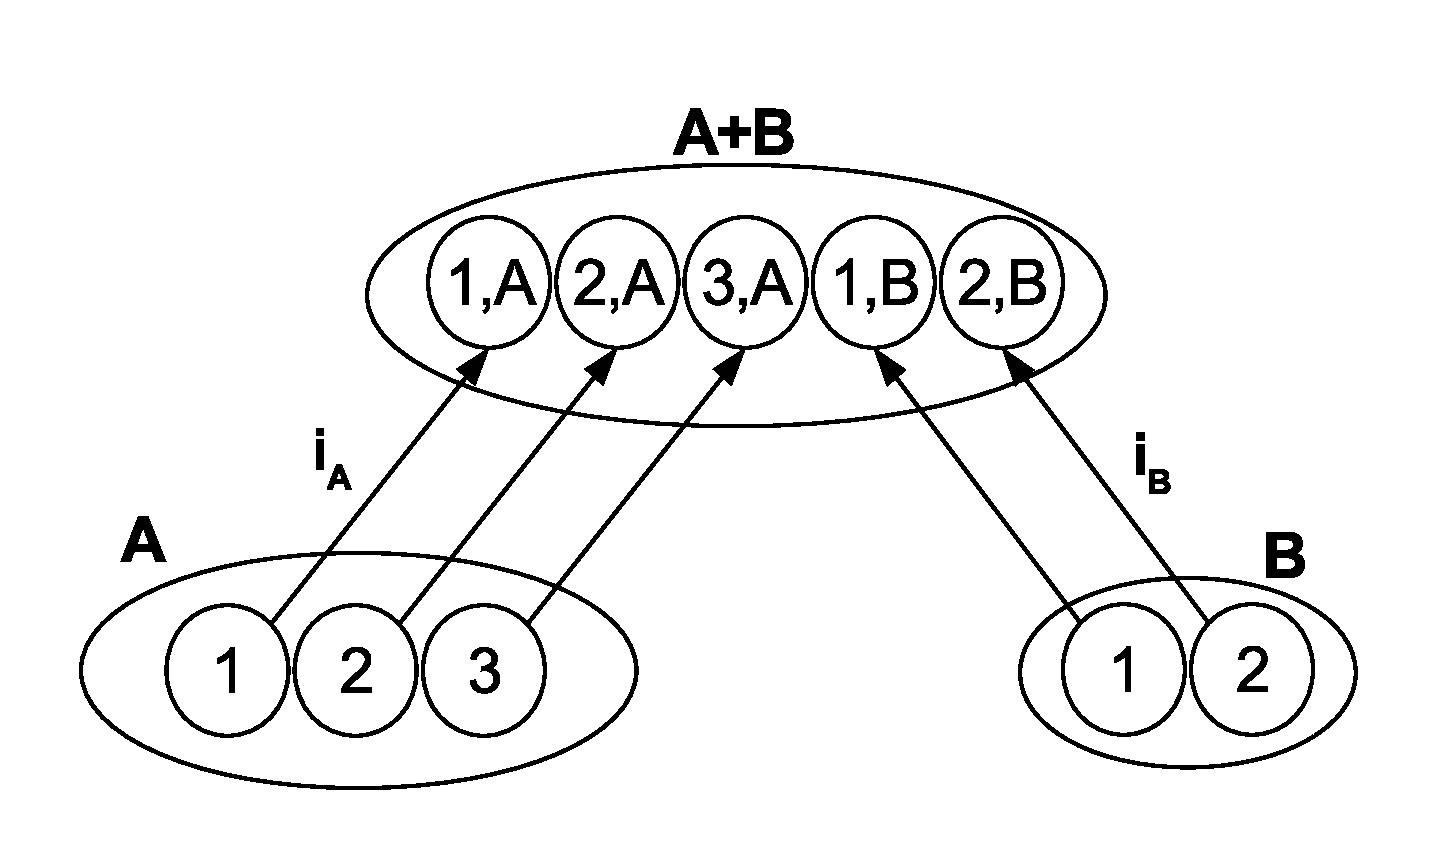
\includegraphics[scale=0.4]{images/gts/coproduct-open}
  \caption{A coproduct in \cat{Set}}\label{fig:gts:coproduct}
\end{figure}


  Take as a candidate a set $C = {(0,A),(1,A),(2,A),(3,A),(1,B},(2,B),(3,B)$. $C$ can not be a coproduct because we can not find a \emph{unique} arrow from $C$ to an arbitrary candidate $X$, as there are multiple choices due to the different possible functions mapping $A$ and $B$ to $C$. Also, an object such as $D = \{(1,A),(2,AB),(3,A),(1,B)\}$ can not be a coproduct because it is not possible to find an arrow from $D$ an $X$ such that the diagram commutes, because all the possible functions from $A$ and $B$ would identify some elements of the sources.

  Notice that $(A+B)' = \{(1,0),(2,0),(3,0),(1,1),(2,1)\}$ or $(A+B)'' = \{a,b,c,d,e\}$ or any other set with five elements would be equally valid as coproducts for this case. This is due to the fact the categories deal with their objects up to isomorphism, i.e. all this objects have the same format regardless of their internal representations.
\end{example}


\begin{definition}[Coequalizer] Given two objects $A$ and $B$ with two parallel morphisms \morph{f}{A}{B} \morph{g}{A}{B}, the coequalizer of the diagram is an object $X$ together with a morphism \morph{h}{B}{X} such that \mbox{$h \circ f = h \circ g$} and, for any other such objects $X'$ with a morphism $h'$, there is a unique morphism \morph{!}{X}{X'} such that the following diagram commutes.

\diagram{
  A\ar@<.5ex>[r]^{f}\ar@<-.5ex>[r]_{g} & B\ar[r]^{h}\ar[dr]_{h'} & X\ar@{.>}[d]^{!}\\
    &   & X'
}
\end{definition}

\begin{example}[Coequalizers in \cat{Set}] Coequalizers generalize the notion of smallest equivalence relation. Figure~\ref{fig:gts:coequalizer} shows the coequalizer for two functions from $A$ to $B$, let $f$ be the one represented with a solid line and $g$ the one with a dashed line.

\begin{figure}[!ht]
  \centering
  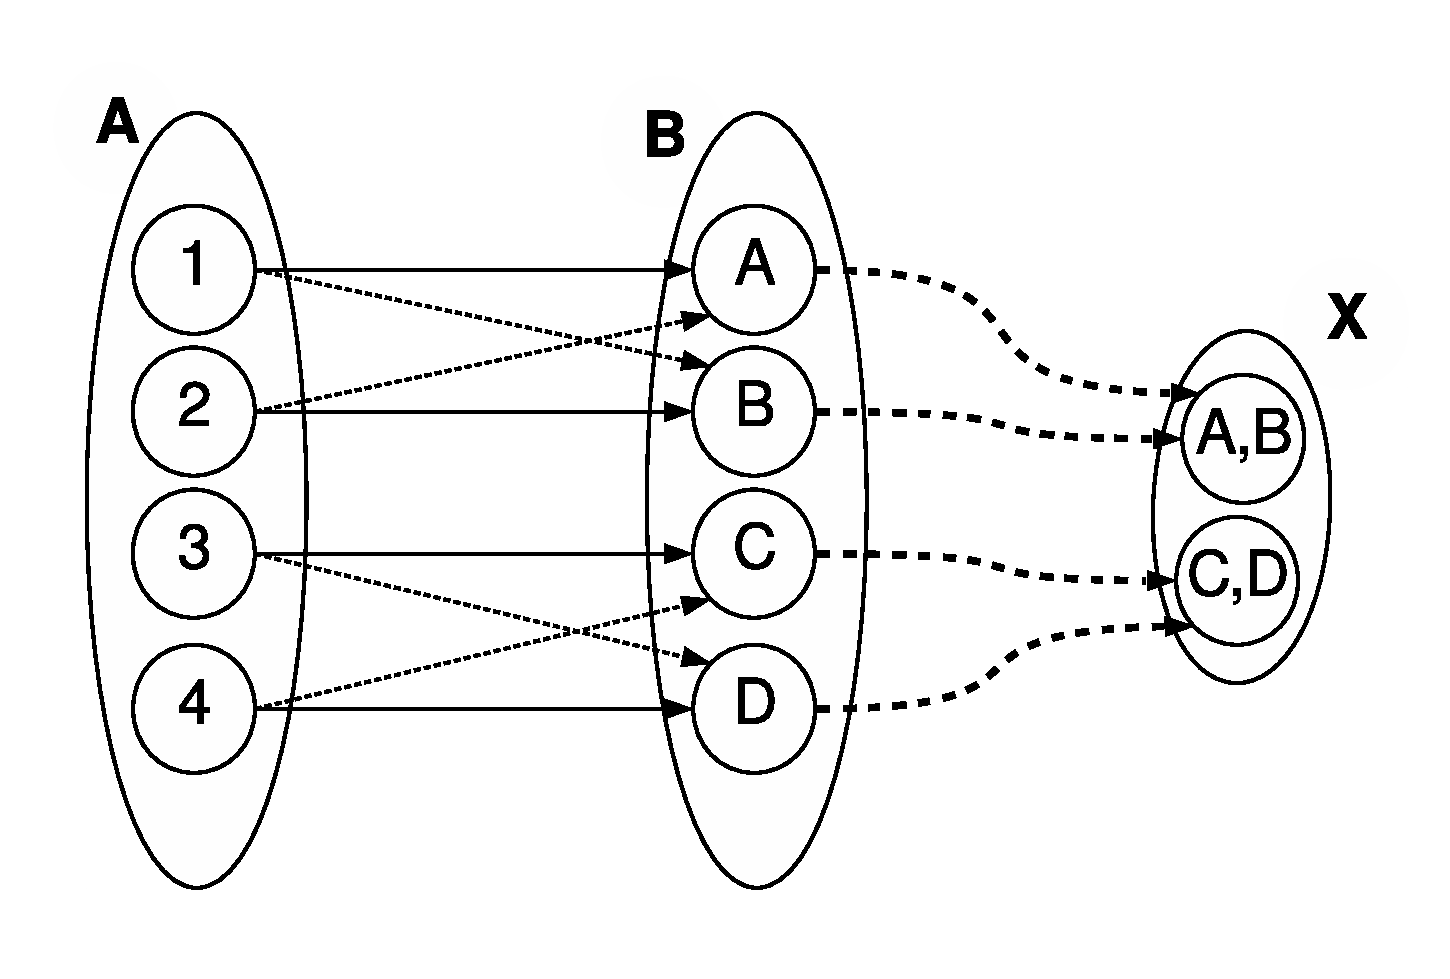
\includegraphics[scale=0.4]{images/gts/coequalizer}
  \caption{A coequalizer in \cat{Set}}\label{fig:gts:coequalizer}
\end{figure}

  It is easy to see that the the function $h$ from $B$ to $X$ corresponds to the equivalence relation that glues together the items that are identified by the functions $f$ and $g$. Notice that $X$ does not contain any other element which is not mapped from $B$ and no element in $X$ was glued together without respecting $f$ and $g$.

\end{example}

\begin{definition}[Pushout] Given a span of arrows \mbox{$B \xleftarrow{f} A \xrightarrow{g} C$}, its \emph{pushout} is an object $X$ together with a pair of arrows \morph{f'}{C}{X} and \morph{g'}{B}{X} such that (1) \mbox{$f' \circ g = g' \circ f$} and (2) for any other object $X'$ with morphisms \morph{i}{B}{X'} and \morph{j}{C}{X'} such that $i \circ f = j \circ g$ there is a unique morphism \morph{!}{X}{X'} such that \mbox{$i =$ $! \circ g'$} and \mbox{$j =$ $! \circ f'$}.

\diagram{
  A\ar[r]^{f}\ar[d]_{g} & B\ar[d]^{g'}\ar@/^1.1pc/[rdd]^{i} &\\
  C\ar[r]_{f'}\ar@/_1.1pc/[drr]_{j}       & X\ar@{.>}[dr]^{!}&\\
                &         &X'
}

\end{definition}

\begin{example}[Pushouts in \cat{Set}] A pushout in \cat{Set} can be seen on Figure~\ref{fig:gts:pushout}. Notice that a pushout maps all elements of sets $B$ and $C$ into set $X$, ``gluing'' the ones that are identified via the morphisms \morph{f}{A}{B} and \morph{g}{A}{C}.

\begin{figure}[!ht]
  \centering
  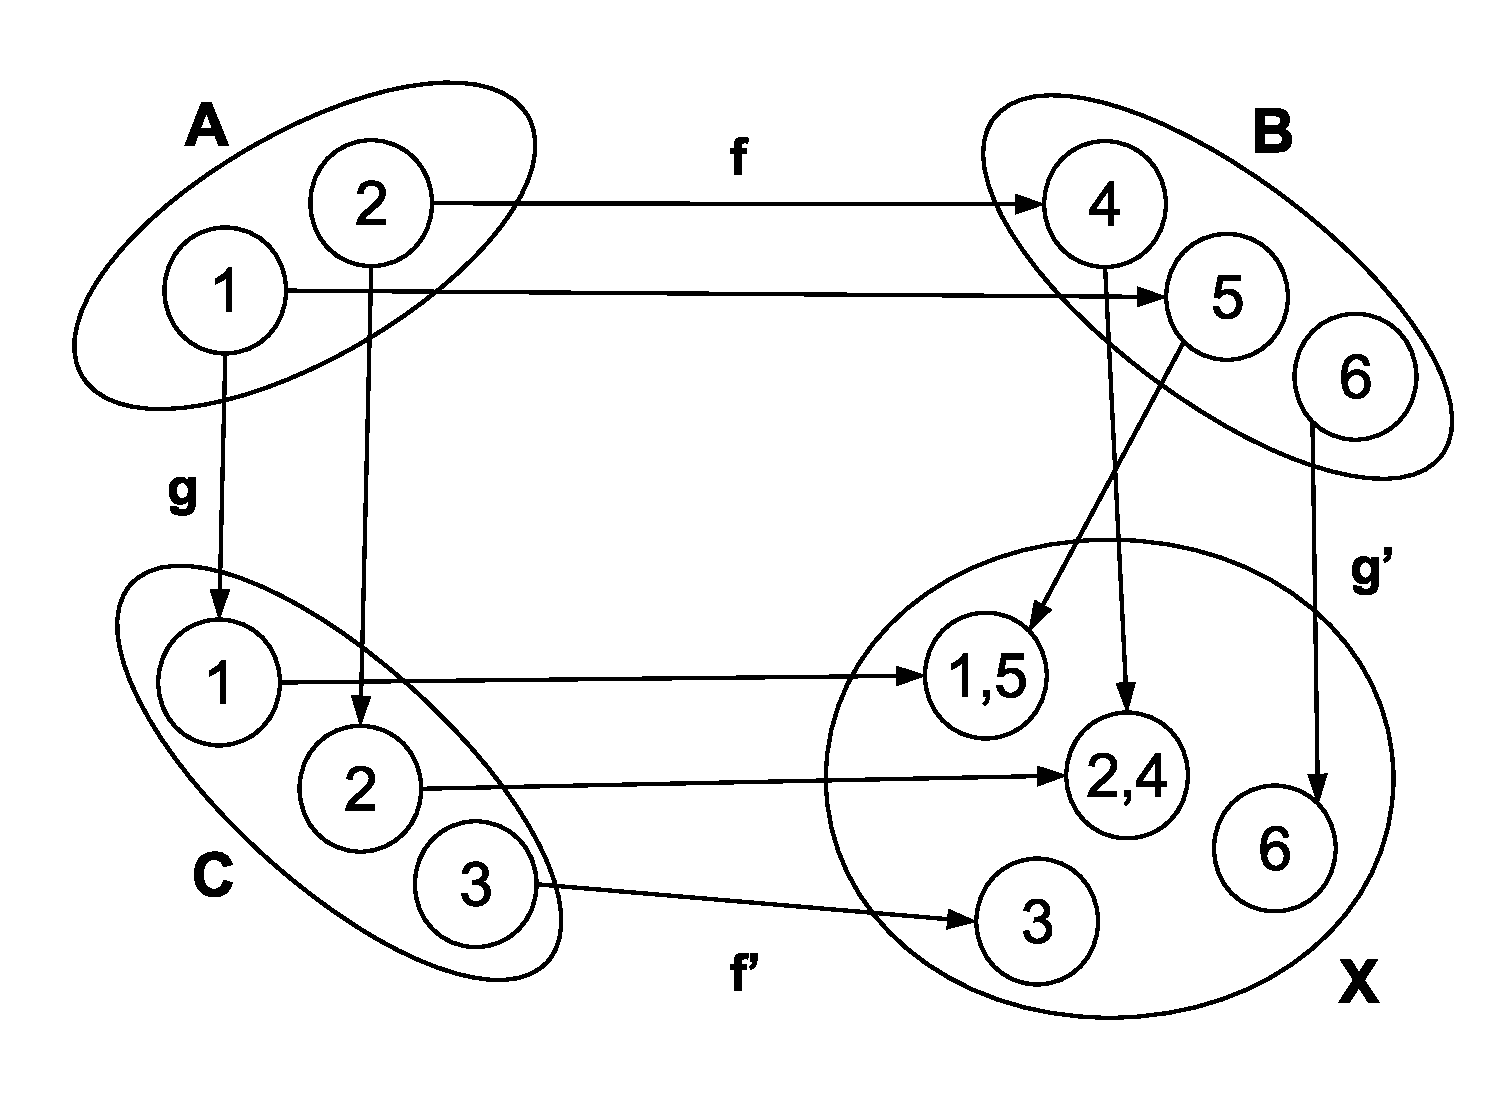
\includegraphics[scale=0.4]{images/gts/pushout}
  \caption{A pushout in \cat{Set}}\label{fig:gts:pushout}
\end{figure}

\end{example}

\begin{definition}[Colimit] Given a diagram $D$ in a category \cat{C}, a \emph{cocone} for $D$ is an object $X$ and a family of morphisms \morph{f_i}{D_i}{X} (one for each object $D_i$ in $D$), such that for each morphism $g$ in $D$ the outer part of the following diagram commutes.

\diagram{
  D_i\ar[rr]^{g}\ar[dr]_{f_i} &   & D_j\ar[dl]^{f_j}\\
      & X &   \\
}
\hfill

  A \emph{colimit} for a diagram $D$ is a cocone \{\morph{f_i}{D_i}{X}\} such that for any other cocone \{\morph{f'_i}{D'_i}{X'}\} there exists a unique morphism \morph{!}{X}{X'} such that the following diagram commutes for every $D_i$ in $D$.


\diagram{
  D_i\ar@/_1.1pc/[ddr]_{f'_i}\ar[rr]^{g}\ar[dr]_{f_i} &   & D_j\ar@/^1.1pc/[ddl]^{f'_j}\ar[dl]^{f_j}\\
      & X\ar@{.>}[d]^{!} &   \\
      & X'&    \\
}
\end{definition}

\begin{example}[Colimits in \cat{Set}] Colimits generalize several constructions such as disjoint unions, direct sums, coproducts, pushouts and others, where different objects of a diagram are ``glued'' together in one single object respecting commutativity.

  All previous examples of coproduct, coequalizer and pushout are special cases of colimits. Figure~\ref{fig:gts:colimit} shows a colimit for a diagram that can not be calculated in (one step) by any of the previous constructions.

\begin{figure}[!ht]
  \centering
  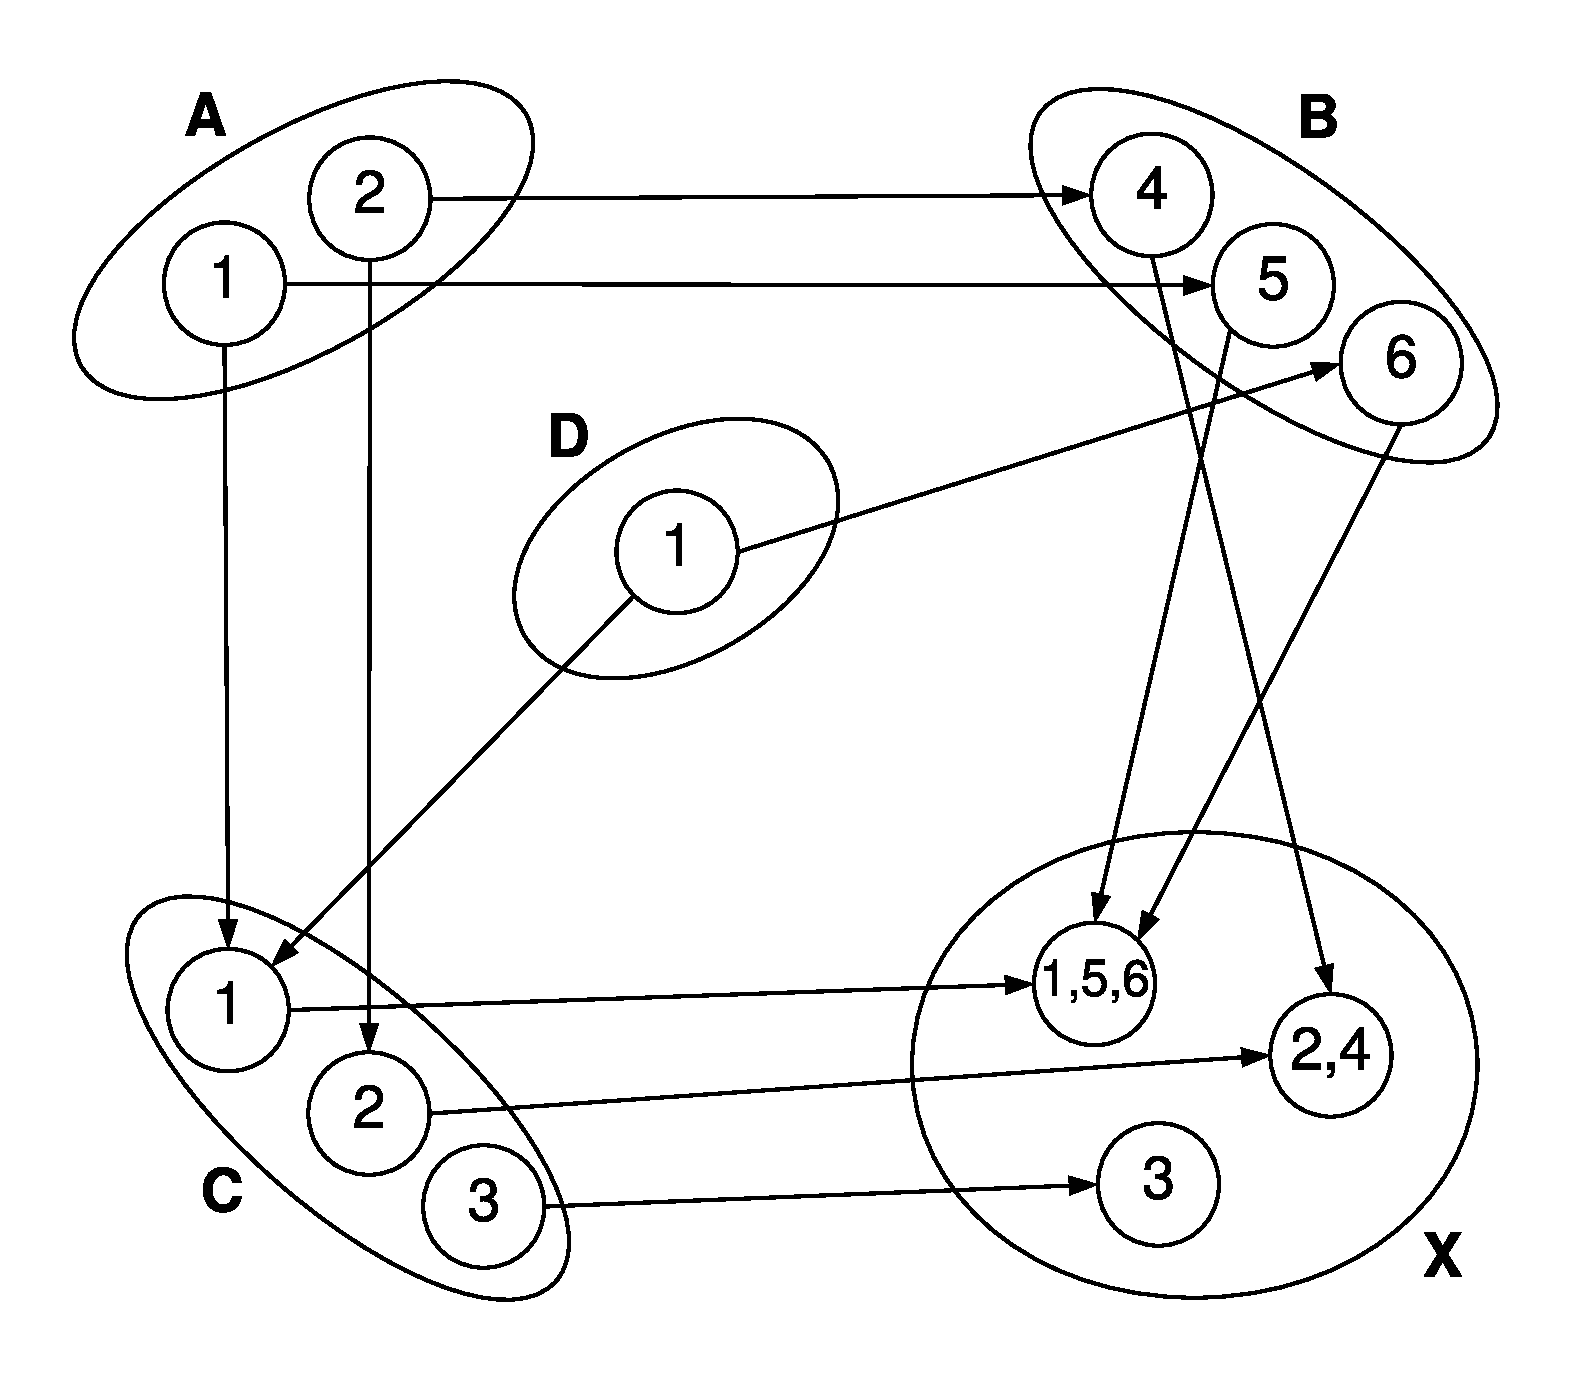
\includegraphics[scale=0.4]{images/gts/colimit}
  \caption{A colimit in \cat{Set}}\label{fig:gts:colimit}
\end{figure}

\end{example}


\iffalse
\begin{definition}[Pullback] \tinytodo{Maintain only if we are going to use the concurrent rules chapter} Given 

\diagram{
  X'\ar@{.>}[dr]^{!}\ar@/^1.1pc/[rrd]^{i}\ar@/_1.1pc/[ddr]_{j}  & &\\
  & X\ar[r]^{g'}\ar[d]_{f'} & B\ar[d]^{f}\\
  & C\ar[r]_{g}      & A
}
\end{definition}

\begin{example}[Pullbacks in \cat{Set}]
\end{example}
\fi

\section{Graph Grammars}

The theory of graph grammars and graph transformation systems is based on the application of rules that are able to modify graphs. Using this framework, it is possible to model complex systems as graph transformation systems, where graphs represent the system states and the rules model transitions between states.

Graph grammars have a wide application in computer science, not only because graphs are very natural and intuitive way to model complex situations, but also because it is possible to reason about several properties of the modelled systems using its formalism~\cite{Ehrig2006,Rozenberg1997}.

We now review the basic concepts and analysis techniques for graph transformations that are used in this work.

\begin{definition}[Graph] A graph is a tuple $G = \left(V,E,s,t\right)$ where: $V$ is a set of nodes, $E$ is a set of Edges and $s,t : E \rightarrow V$ are two total functions that map each edge in $E$ to its source and target in $V$.

\end{definition}

\begin{example}[Graph]\label{def:graph} Figure~\ref{fig:gts:graph} shows a simple graph $G$ with $V = \{1,2,3,4\}$, $E = \{1,2\}$, $s =\{(1,1),(2,3)\}$ and $t = \{(1,2),(2,3)\}$.
\begin{figure}[!ht]
  \centering
  
\includegraphics[scale=0.8]{images/gts/graph}
  \caption{A graph example}\label{fig:gts:graph}
\end{figure}
\end{example}

\begin{definition}[Graph Morphism]\label{def:graph-morphism} Given two graphs $G_1,G_2$ with \mbox{$G_i = \left(V_i, E_i, s_i, t_i\right)$} for $i$ in $[1,2]$, a graph morphism $f : G_1 \rightarrow G_2$ between them is a pair $f = \left(f_V,f_E\right)$ where $f_V : V_1 \rightarrow V_2$ and $f_E : E_1 \rightarrow E_2$ are total functions that preserve the source and target functions, i.e. $f_V \circ s_1 = s_2 \circ f_E$ and $f_V \circ t_1 = t_2 \circ f_E$.
\end{definition}

\begin{example}[Graph Morphisms]Figure~\ref{fig:gts:compact-graph-morphism} shows three morphisms $f : G_0 \rightarrow G_1$, $g : G_0 \rightarrow G_2$ and $h : G_0 \rightarrow G_3$, which are a monomorphism, an epimorphism and a isomorphism, respectively.

  The morphism $f$ maps node $\Circle_1$ to $\Circle_a$, node $\Circle_2$ to $\Circle_b$ and edge $\curvearrowleft_1$ to $\curvearrowleft_q$; $g$ maps both nodes $\Circle_1$ and $\Circle_2$ to $\Circle_c$ and edge $\curvearrowleft_1$ to $\curvearrowleft_r$; and $h$ maps node $\Circle_1$ to $\Circle_d$, node $\Circle_2$ to $\Circle_e$ and edge $\curvearrowleft_1$ to $\curvearrowleft_s$.

  Figure~\ref{fig:gts:expanded-graph-morphism} shows the morphism $f$ in an expanded (explicit) notation. Both notations will be used through this work, according to which one will be the better to clarify the meaning at the moment.
\begin{figure}[!ht]
  \centering
  \fbox{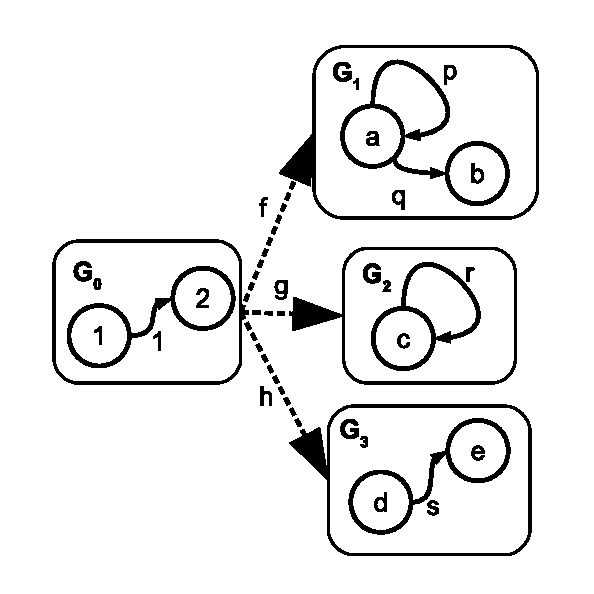
\includegraphics[scale=0.8]{images/gts/compact-graph-morphism}}
  \caption{A graph morphism example}\label{fig:gts:compact-graph-morphism}
\end{figure}

\begin{figure}[!ht]
  \centering
  \fbox{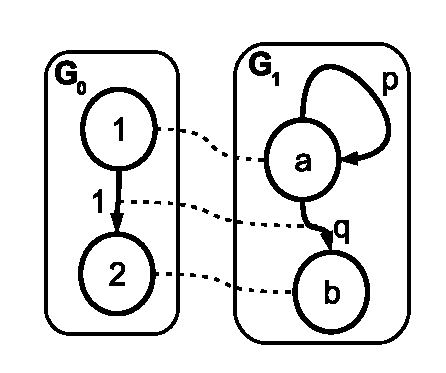
\includegraphics[scale=0.8]{images/gts/expanded-graph-morphism}}
  \caption{An expanded graph morphism example}\label{fig:gts:expanded-graph-morphism}
\end{figure}
\end{example}

\begin{definition}[Typed Graph and Typed Graph Morphism] A type graph is a distinguished graph $TG = \left(V_{TG},E_{TG},s_{TG},t_{TG}\right)$ where $V_{TG}$ and $E_{TG}$ are called the node and edge type alphabets, respectively.

  A typed graph is a pair $G^T = \left(G, type\right)$ consisting of a graph $G$ and a graph morphism $type : G \rightarrow TG$.

  Given two typed graphs $G^T_1 = \left(G_1,type_1\right)$ and $G^T_2 =\left(G_2,type_2\right)$, a typed graph morphism $f : G^T_1 \rightarrow G^T_2$ is a graph morphism $f : G_1 \rightarrow G_2$ such that $type_2 \circ f = type_1$:

\diagram{
  G_1\ar[rr]^{f}\ar[dr]_{type_1} & & G_2\ar[dl]^{type_2}\\
  \ar@{}[rur]|{=}& TG &
}
\end{definition}

\begin{example}[Typed Graph and Typed Graph Morphism Example] Figure~\ref{fig:gts:typed-graphs} shows a type graph $T$, and four graphs $G_0, G_1, G_2, G_3$ where only $G_0$ and $G_1$ are valid \emph{T-typed} graphs. 
  
  Notice that $G_2$ can not be a \emph{T-typed} graph because type graph does not have a node of the type $\lozenge$, neither an edge type with source and target in the $\Square$ type. Similarly, $G_3$ is not a valid \emph{T-typed} graph because, although there is an edge type between a $\triangle$ and a $\Square$ types, the source must of this type of edge must be a $\Square$ and the target a $\triangle$.

  Figure~\ref{fig:gts:typed-graph-morphism} shows a typed graph morphism $f : G_0^T \rightarrow G_1^T$, where $f$ maps node $\Circle_a$ to $\Circle_1$, $\Square_b$ to $\Square_1$ and edge $\curvearrowleft_e$ to $\curvearrowleft_2$.
\begin{figure}[!ht]
  \centering
  \fbox{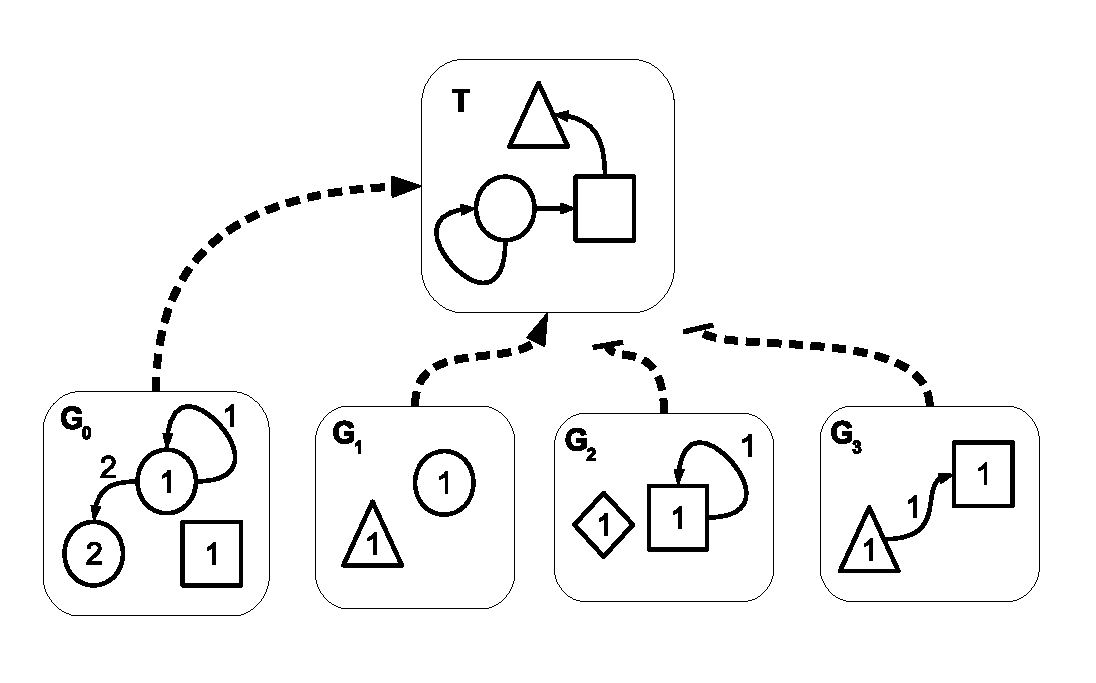
\includegraphics[scale=0.65]{images/gts/typed-graphs}}
  \caption{\emph{T-typed} valid and invalid graphs}\label{fig:gts:typed-graphs}
\end{figure}

\begin{figure}[!ht]
  \centering
  \fbox{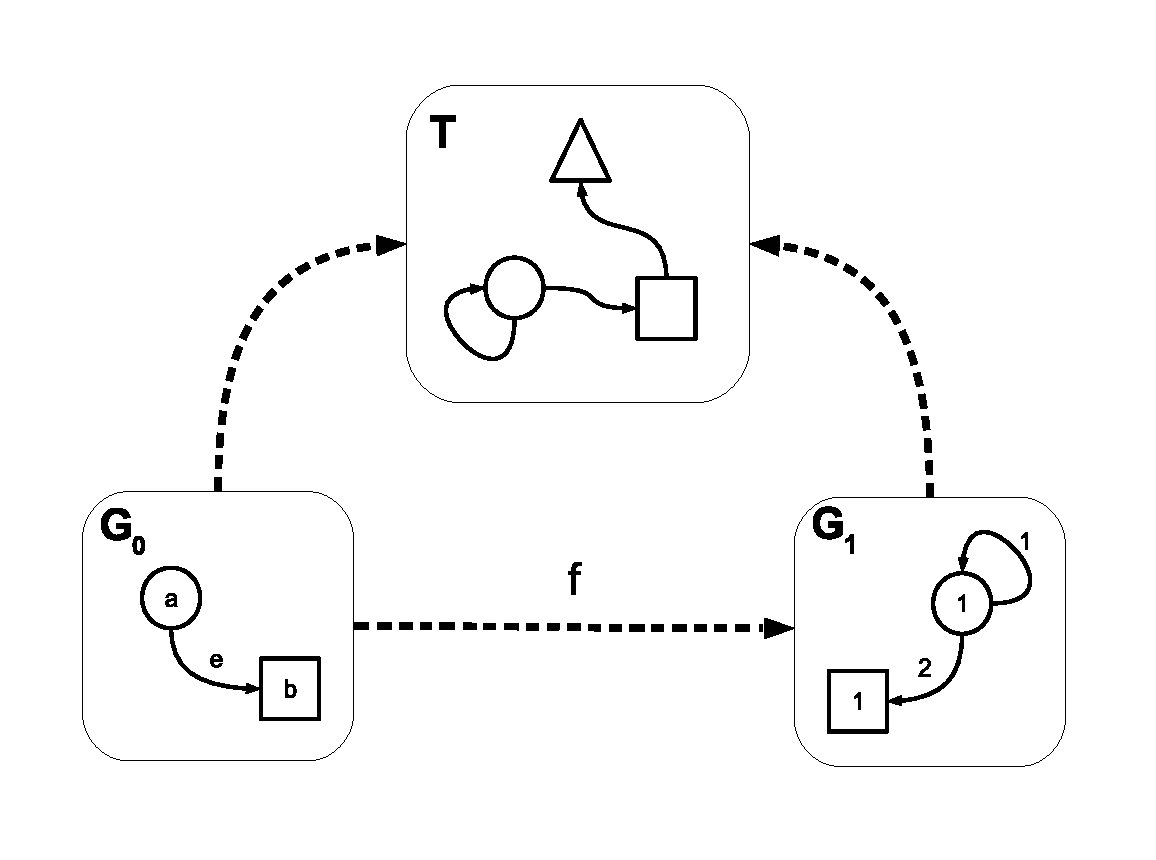
\includegraphics[scale=0.6]{images/gts/typed-graph-morphism}}
  \caption{A typed graph morphism}\label{fig:gts:typed-graph-morphism}
\end{figure}
\end{example}

\begin{remark}[Categories of Graphs and Typed Graphs] We call \cat{Graph} the category whose objects are graphs and arrows are graph morphisms. Similarly, we have that \cat{TGraph_T} is the category whose objects are $T-$typed graphs and whose arrows are $T-$typed graph morphisms.
\end{remark}

\iffalse
\begin{definition}[Positive Atomic Constraint] A \emph{positive} atomic (typed) graph constraint is of the form $PC\left(a\right)$, where $a : P \rightarrow C$ is a (typed) graph morphism. A (typed) graph $G$ satisfies $PC\left(a\right)$ if for every injective (typed) graph morphism $p : P \rightarrow G$ there is at least one injective (typed) graph morphism $q : P \rightarrow C$ such that $p = q \circ a$.

  A positive (typed) graph constraint with $a : \emptyset \rightarrow C$ is also notated $PC\left(C\right)$. Given a (typed) graph $G$, it satisfies $PC\left(C\right)$ if there is an injective (typed) graph morphism $q : C \rightarrow  G$.
\diagram{
  P\ar[rr]^{a}\ar[dr]_{p} & & C\ar[dl]^{q}\\
  \ar@{}[rur]|{=}& G &
}

\end{definition}

\begin{definition}[Negative Atomic Constraint]
A \emph{negative} atomic (typed) graph constraint is of the form $NC\left(a\right)$, where $a : P \rightarrow C$ is a (typed) graph morphism. A (typed) graph $G$ satisfies $PC\left(a\right)$ if for every injective (typed) graph morphism $p : P \rightarrow G$ there is no injective (typed) graph morphism $q : P \rightarrow C$ such that $p = q \circ a$.

  A negative (typed) graph constraint with $a : \emptyset \rightarrow C$ is also notated $NC\left(C\right)$. Given a (typed) graph $G$, it satisfies $NC\left(C\right)$ if there is no injective (typed) graph morphism $q : C \rightarrow G$.

\diagram{
  P\ar[rr]^{a}\ar[dr]_{p} & & C\ar[dl]|{|}^{q}\\
  \ar@{}[rur]|{=}& G &
}

\end{definition}

\begin{remark} It was shown in ~\cite{Ehrig2006} that negative atomic constraints do not give more expressive power. However, we introduced this concept because it makes easier to reason about some of the purposes of this thesis in a negative rather than a positive manner.%\tinytodo{related to the graph constraint definition, maybe this is not necessary}
\end{remark}

\begin{definition}[Graph Constraint] A (typed) graph constraint is a \emph{boolean} formula over atomic (typed) graph constraints, in such way that $true$, $false$ and every atomic constraint are also graph constraints. Also, if $c$ and $c_i$, with $i \in I$ for some index set $I$, are graph constraints, then $\neg c$, $\land_{i \in I} c_i$ and $\lor_{i \in I} c_i$ are also graph constraints.

  A graph $G$ satisfies a graph constraint $c$ (written $G \models c$) iff one of the following situations occurs:
  \begin{itemize}
    \item $c = true$
    \item $c$ is an atomic constraint $a$ and $G \models a$
    \item $c = \neg c'$ and $G \not\models c'$
    \item $c = \land_{i \in I}c_i$ and $G \models c_i$ $\forall i \in I$ 
    \item $c = \lor_{i \in I}c_i$  and $\exists i \in I$ such that $G \models c_i$
  \end{itemize}
\end{definition}

\begin{example}[Constraints Example]
\end{example}
\fi

\begin{definition}[Graph Rule]\label{def:graph-rule} A (typed) graph rule\footnote{Also called graph transformation rule or graph production.} \graphrule{} is a span of (typed) graph monomorphisms \lefthand{} and \righthand{}  where the (typed) graphs $L$, $K$ and $R$ are called the left-hand side, gluing graph and right-hand side, respectively.

  Given a (typed) graph rule $p$, its inverse rule is defined by \inversegraphrule.
\end{definition}

\begin{example}[Graph Rule Example and Notation] Figure~\ref{fig:gts:rule} shows an example of a graph rule which reads a node of the type $\Circle$, deletes a node of the type $\triangle$ and then creates a node of the type $\Square$ with an edge between the $\Circle$ and the \Square. 
  
Figure~\ref{fig:gts:rule-standard} presents the rule in the standard DPO notation, while Figure~\ref{fig:gts:rule-compact} depicts the same rule in a compact notation, where the gluing graph is omitted. 

Sometimes we will use the compact notation to make the figures smaller. Notice that the compact notation does not cause any semantic loss as the gluing graph can be obtained as the ``intersection'' between the left and right graphs, and the morphisms $l$ and $r$ as the inclusions of $K$ in $L$ and $R$, respectively.

\begin{figure}[!ht]
  \centering
  \begin{subfigure}[t]{.5\textwidth}
    \centerline{\fbox{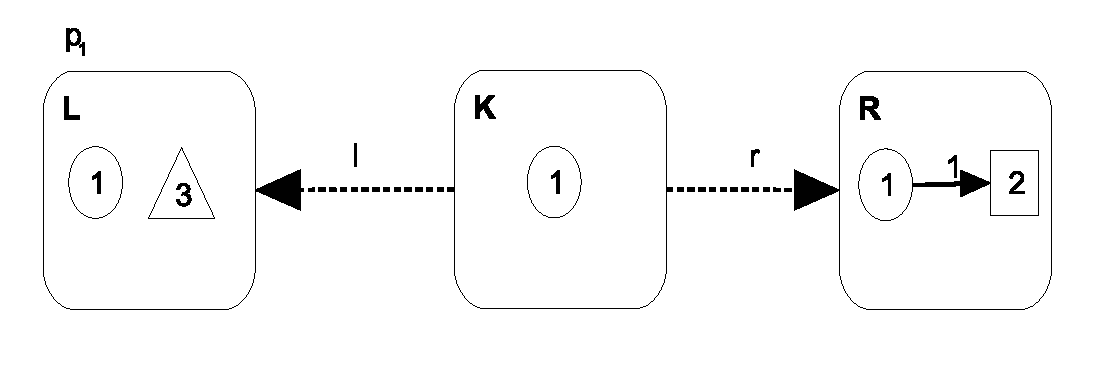
\includegraphics[scale=0.5]{images/gts/standard-dpo-rule}}}
    \caption{Standard DPO rule notation}\label{fig:gts:rule-standard}
  \end{subfigure}

  \begin{subfigure}[t]{.5\textwidth}
    \centerline{\fbox{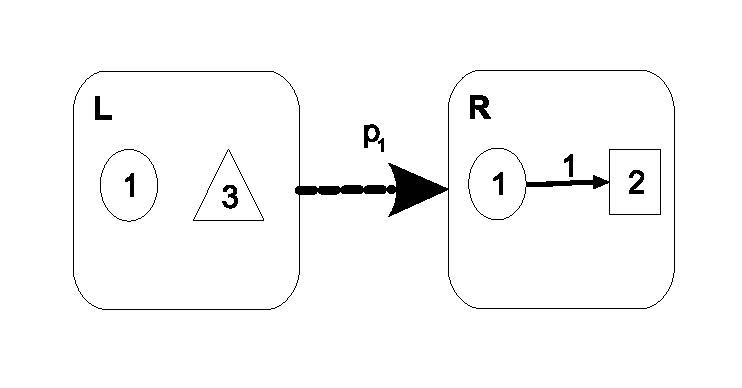
\includegraphics[scale=0.5]{images/gts/compact-dpo-rule}}}
    \caption{Compact DPO rule notation}\label{fig:gts:rule-compact}
  \end{subfigure}
  \caption{DPO graph rule}\label{fig:gts:rule}
\end{figure}
\end{example}

\begin{definition}[Graph Transformation] Given a (typed) graph rule \graphrule{} and a (typed) graph $G$ with a (typed) graph morphism \match, called match, a direct (typed) graph transformation $G \xRightarrow{p,m} H$ from $G$ to a (typed) graph $H$ is a double-pushout (DPO) diagram such as:

\diagram{
  L\ar[d]_{m}        & & K\ar[ll]_{l}\ar[rr]^{r}\ar[d]|{k} & & R\ar[d]^{m'}\\
  G\ar@{}[urr]|{\left(1\right)} & & D\ar[ll]^{f}\ar[rr]_{g}             & & H\ar@{}[ull]|{\left(2\right)}
}

  For \cat{TGraph_T} there are two conditions, called \emph{gluing conditions}, that must be satisfied so that the pushouts (1) and (2) exist and the rule graph rule can be applied:
  
  First, the \emph{dangling condition} requires that no node can be deleted if it has incident edges that are not also deleted (otherwise the result of this deletion would not be a graph).  Second, the \emph{identification condition} requires the match to not identify a deleted element with a preserved or (another) deleted one.
\end{definition}

\begin{example}[Graph Transformation Examples] Figure~\ref{fig:gts:transformation-success} shows a transformation where the rule depicted in Figure~\ref{fig:gts:rule} is successfully applied over a graph instance $G_0$.

  Figure~\ref{fig:gts:transformation-fail} shows the same rule being applied over a graph instance $G_1$ which does not satisfy the gluing conditions, more specifically it does not satisfy the dangling condition.

\begin{figure}[!ht]
  \centering
  \begin{subfigure}[t]{.5\textwidth}
    \centerline{\fbox{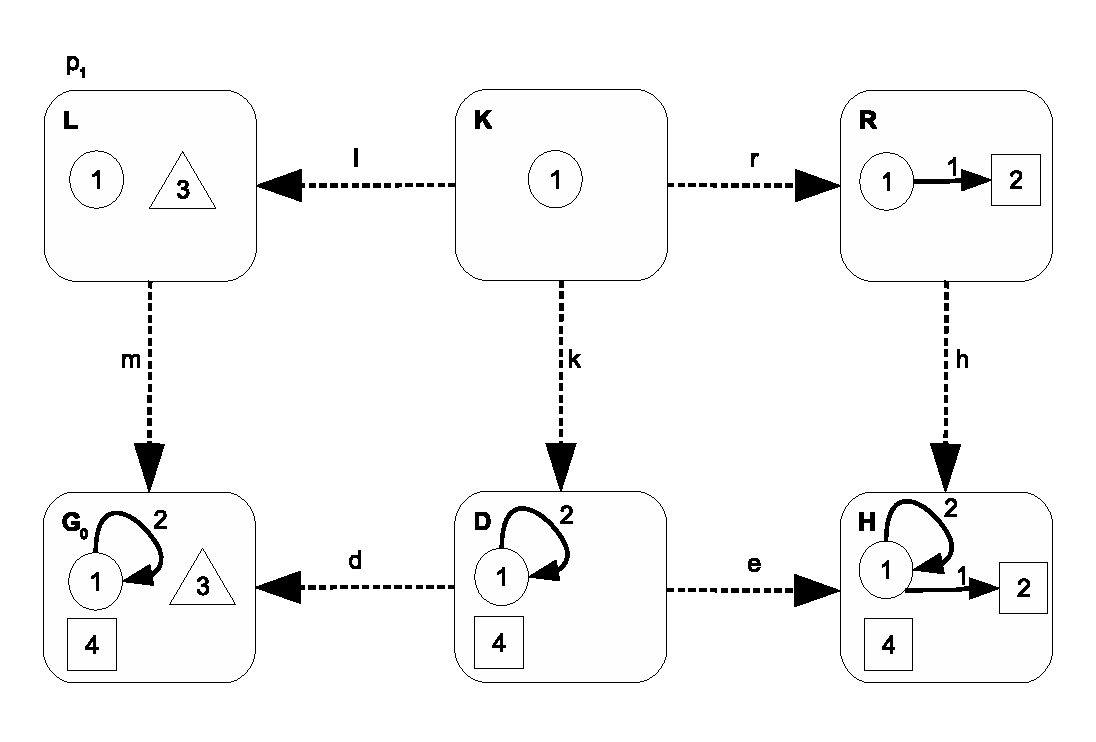
\includegraphics[scale=0.8]{images/gts/transformation}}}
    \caption{Successfully applied graph transformation}\label{fig:gts:transformation-success}
  \end{subfigure}

  \begin{subfigure}[t]{.5\textwidth}
    \centerline{\fbox{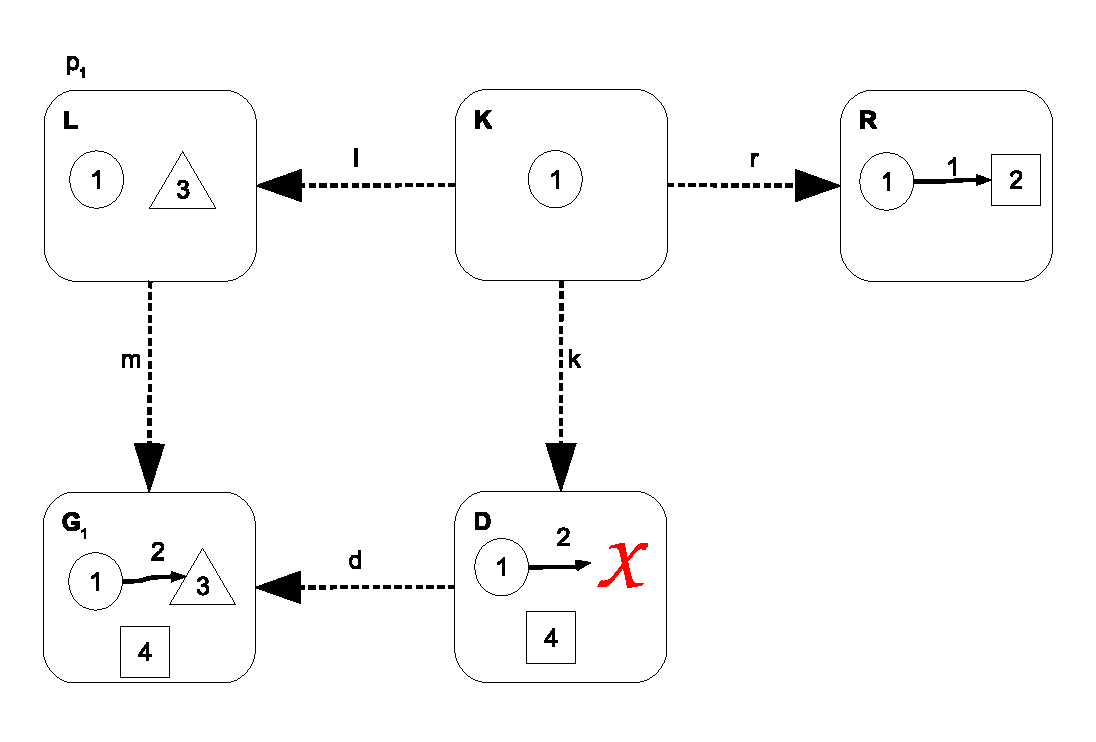
\includegraphics[scale=0.8]{images/gts/transformation-failed}}}
    \caption{Failing graph transformation due to the dangling condition}\label{fig:gts:transformation-fail}
  \end{subfigure}
  \caption{Graph transformation}\label{fig:gts:transformation}
\end{figure}

\end{example}
\begin{definition}[Negative Application Condition] A \emph{left} negative application condition over a graph rule \graphrule{} is of the form $NAC\left(n\right)$, where \nac{} is an arbitrary (typed) graph morphism. A match \match{} of a rule $p$ satisfies\footnote{When a NAC is satisfied it is also said that the NAC is \emph{not triggered} and vice versa.} $NAC\left(n\right)$ on $L$, written $m \models NAC\left(n\right)$, iff $\nexists$ $q : N \rightarrow G$ with $q$ injective and $q \circ n = m$.

\diagram{
  N\ar@{.>}[dr]|{|}_{q} & L\ar[d]^{m}\ar[l]_{n}\\
   & G
}

  A match \match{} satisfies a set \mbox{$NAC_L = \{NAC\left(n_i\right)|i \in I\}$} of left $NACs$, iff \mbox{$m \models NAC\left(n_i\right)$} $\forall i \in I$.

  Analogously, a \emph{right} negative application condition over a graph rule \graphrule{} is of the form $NAC\left(n\right)$, where \rightnac{} is an arbitrary (typed) graph morphism. A comatch \comatch{} of a rule $p$ satisfies $NAC\left(n\right)$ on $R$ (written \mbox{$m' \models NAC\left(n\right)$}) iff $\nexists$ $q : N \rightarrow H$ with $q$ injective and $q \circ n = m'$.

\diagram{
  R\ar[d]_{m'}\ar[r]^{n} & N\ar@{.>}[dl]|{|}^{q}\\
  H &
}
  Also, a comatch \comatch{} satisfies a set \mbox{$NAC_R = \{NAC\left(n_i\right)|i \in I\}$} of right $NACs$, iff $m' \models NAC\left(n_i\right)$ $\forall i \in I$.

\end{definition}

\begin{example}[NAC and NAC satisfiability] Figure~\ref{fig:gts:nacs:satisfied} shows a NAC that is satisfied (i.e. not triggered) over a match $m$, as there is no possible way of mapping the edge between $\Circle_1$ and $\Square_1$ in $N$ to an edge in $G_0$ such that the resulting triangle commutes. Therefore, if $G_0$ also satisfies the gluing conditions for the corresponding rule the transformation can be applied.

  On the other hand, Figure~\ref{fig:gts:nacs:triggered} shows a NAC that is triggered (i.e. not satisfied) over the match $m$: all the elements in $N$ can be mapped to $G_0$ such that the resulting triangle commutes. Therefore, even if $G_0$ satisfies the gluing conditions, the transformation can not be applied, as the pattern forbidden by the NAC was found on the instance graph.

\begin{figure}[!ht]
  \centering
  \begin{subfigure}[t]{.5\textwidth}
    \centerline{\fbox{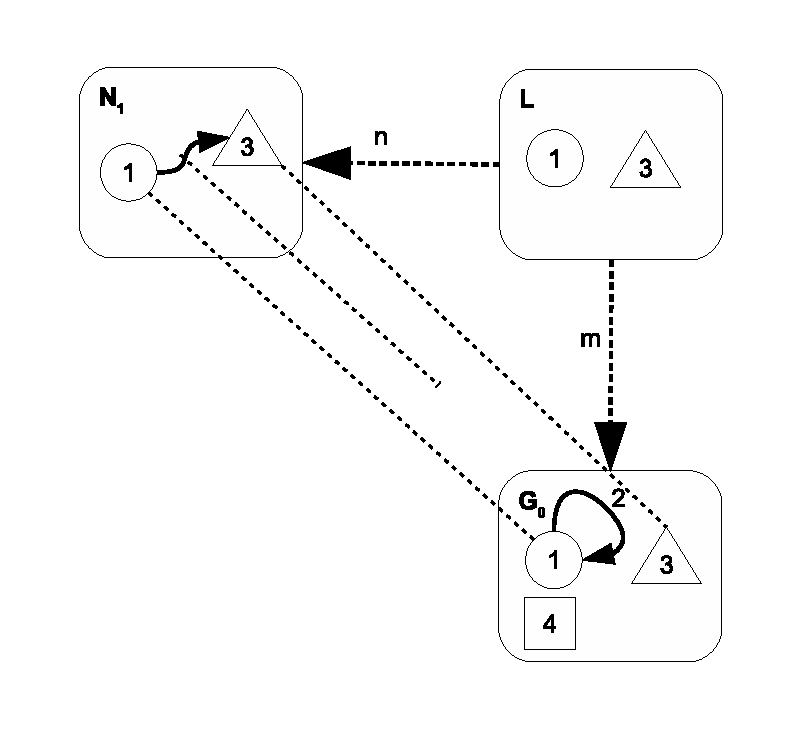
\includegraphics[scale=0.55]{images/gts/satisfied_nac}}}
    \caption{A satisfied NAC}\label{fig:gts:nacs:satisfied}
  \end{subfigure}%
  \begin{subfigure}[t]{.5\textwidth}
    \centerline{\fbox{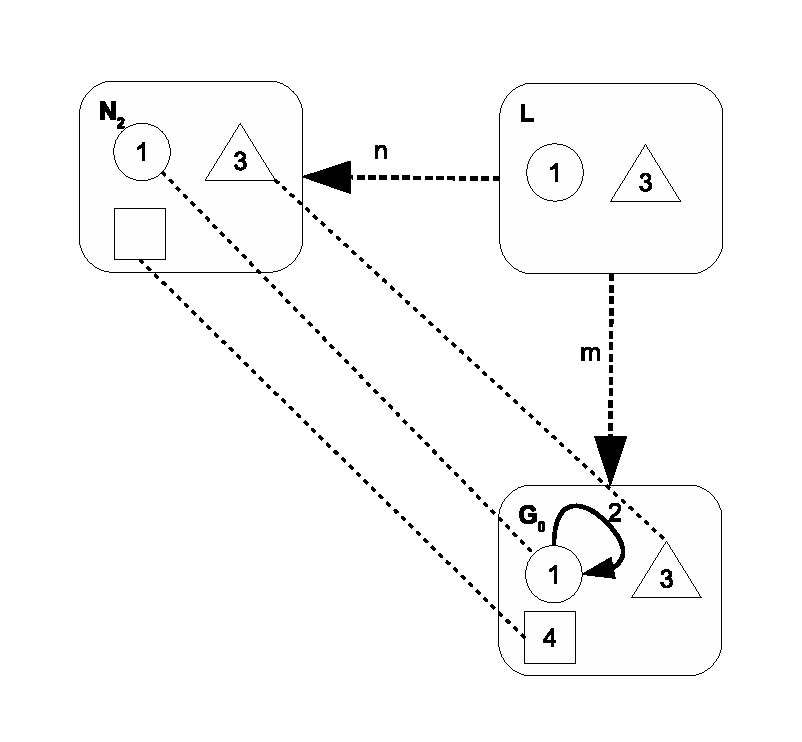
\includegraphics[scale=0.55]{images/gts/triggered_nac}}}
    \caption{A triggered NAC}\label{fig:gts:nacs:triggered}
  \end{subfigure}
  \begin{subfigure}[t]{.5\textwidth}
    \centerline{\fbox{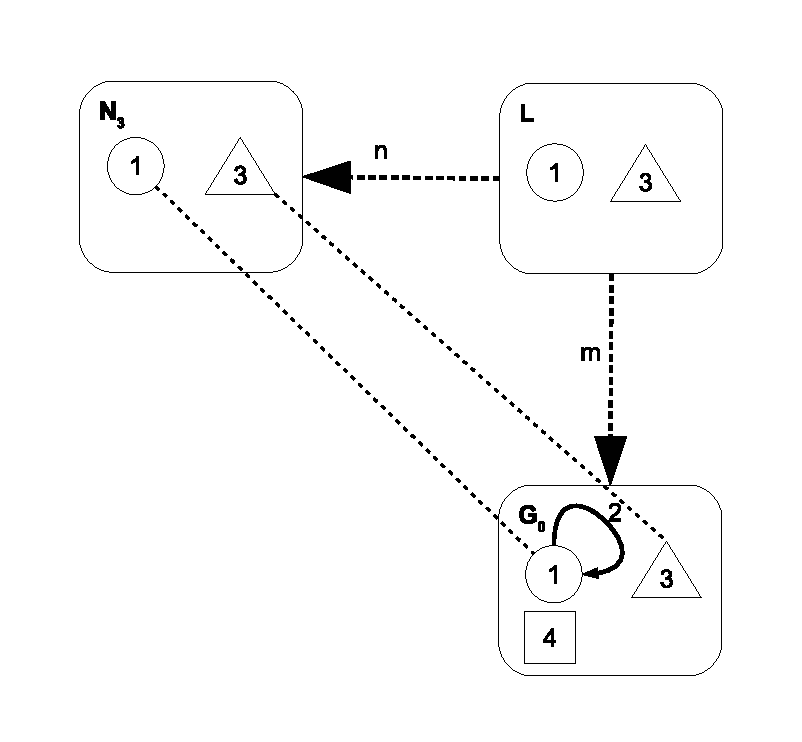
\includegraphics[scale=0.55]{images/gts/trivially_triggered_nac}}}
    \caption{A trivially-triggered NAC}\label{fig:gts:nacs:trivial}
  \end{subfigure}
  \caption{NACs and NAC satisfiability}\label{fig:gts:nacs}
\end{figure}
\end{example}

%\begin{assumption}[Left NACs] Unless stated otherwise, we will work with graph rules that have only left $NACs$ for the rest of this thesis. This is without loss of generality once right $NACs$ can be translated to left ones as it is shown in Definition~\ref{def:shift-nac}.
%\end{assumption}

\begin{definition}[Trivially-Triggered NACs] Given a $NAC(n)$, where $n : L \rightarrow \hat{L}$ is a isomorphism, and a match \match{} which is also a monomorphism, we call $NAC(n)$ a \emph{trivially-triggered NAC} as, for every monomorphic $m$, there will always exist a $q : \hat{L} \rightarrow G$ injective such that $q \circ n = m$.

  A trivially-triggered NAC $n : L \rightarrow \hat{L}$ is also notated $NAC(L)$. If a rule $p$ has a trivially-triggered NAC then $p$ can never be applied whatsoever, as the NAC will never be satisfied. An example of a trivially-triggered NAC is shown on Figure~\ref{fig:gts:nacs:trivial}.
\end{definition}

\begin{definition}[Graph Transformation System and Graph Grammar] A typed graph transformation system is a pair $GTS = \left(TG,P\right)$ where $TG$ is the type graph of the system and $P$ is a set of typed graph rules with NACs.

  A typed graph grammar is a pair $GG = \left(GTS,I\right)$ where $TGS$ is a typed graph transformation system and $I$ is a typed start graph. It can also be notated as $GG = \left(TG, I^{TG},P \right)$.

\end{definition}

\begin{example}[Mail Server Graph Transformation System] Fig~\ref{fig:gts:mail} depicts a graph transformation system that models a client-server scenario for a very simple e-mail application. This system has only four actions: 

\begin{enumerate}
  \item \emph{sendMessage}: a client sends a message to a server,\tinytodo{fix arrow direction}
  \item \emph{getData}: a piece of data is obtained from a server,
  \item \emph{receiveMessage}: a server sends a message to a client,
  \item \emph{deleteMessage}: a client obtains a piece of data from a received message and the message is destroyed.
\end{enumerate}

\begin{figure}[!ht]
  \centering
  \begin{subfigure}[t]{.5\textwidth}
    \centerline{\fbox{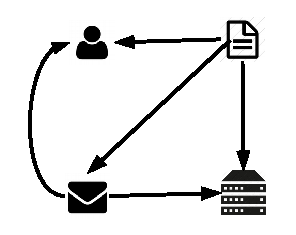
\includegraphics[scale=0.5]{gts/grammar/grammar-type-graph}}}
    \caption{Type Graph}
  \end{subfigure}
  \begin{subfigure}[t]{.5\textwidth}
    \centerline{\fbox{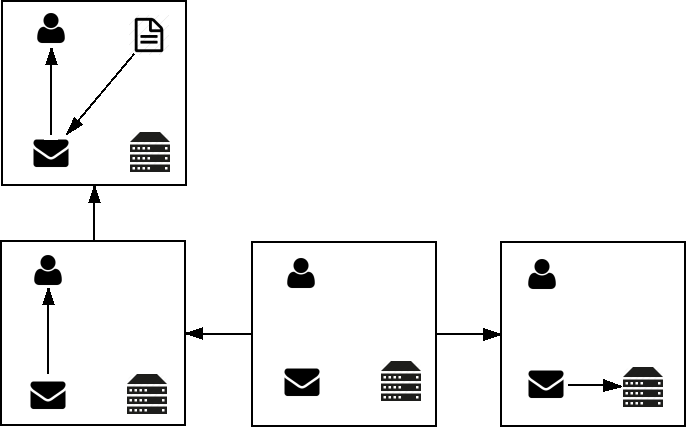
\includegraphics[scale=0.3]{gts/grammar/sendMessage}}}
    \caption{Send message}
  \end{subfigure}%
  \begin{subfigure}[t]{.5\textwidth}
    \centerline{\fbox{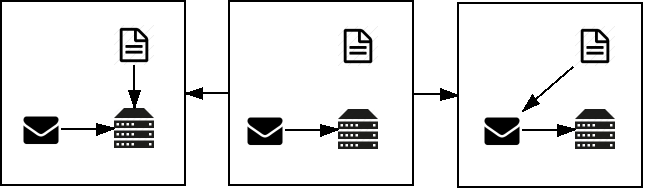
\includegraphics[scale=0.3]{gts/grammar/getData}}}
    \caption{Get data}
  \end{subfigure}
  \begin{subfigure}[t]{.5\textwidth}
    \centerline{\fbox{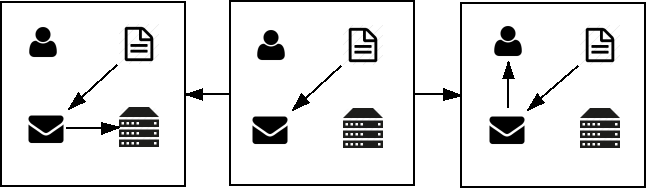
\includegraphics[scale=0.3]{gts/grammar/receiveMessage}}}
    \caption{Receive message}
  \end{subfigure}%
  \begin{subfigure}[t]{.5\textwidth}
    \centerline{\fbox{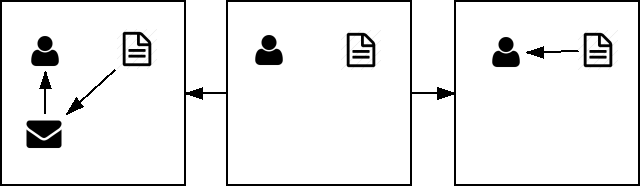
\includegraphics[scale=0.3]{gts/grammar/deleteMessage}}}
    \caption{Delete message}
  \end{subfigure}
  \caption{Mail application graph transformation system}\label{fig:gts:mail}
\end{figure}

\iffalse
\begin{figure}
\centering
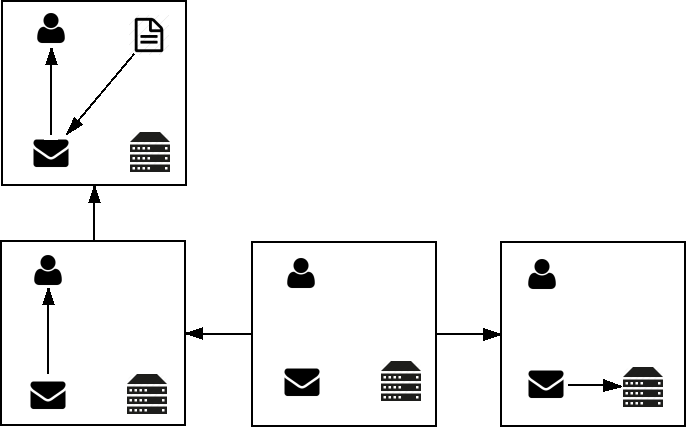
\includegraphics[width=6.5cm]{gts/grammar/sendMessage}
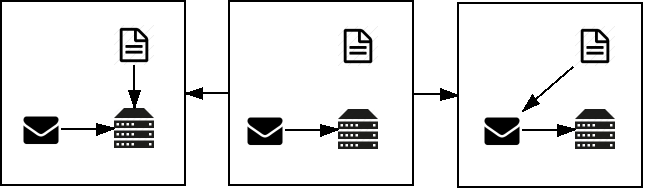
\includegraphics[width=5cm]{gts/grammar/getData}
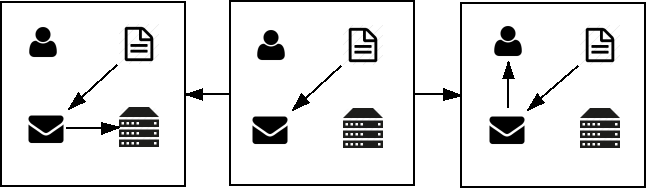
\includegraphics[width=5cm]{gts/grammar/receiveMessage}
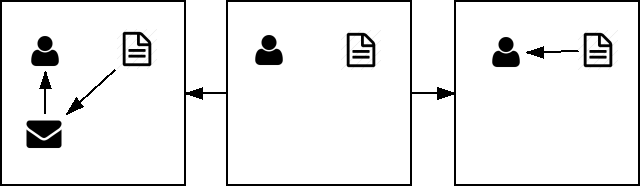
\includegraphics[width=5cm]{gts/grammar/deleteMessage}
\caption{\label{fig:gts:mail} Graph rules for Server}
\end{figure}
\fi
\end{example}

\section{Parallel and Sequential Independence}

One of the characteristics that make Graph Transformation Systems and Graph Grammars suitable formalisms to model and reason about parallel and/or concurrent systems is the possibility to check whether the transformations given by two graph rules over the same instance graph can be applied (1) at the same time or (2) in any interchangeable order. In the first case we say that the transformations are parallel independent; in the later we say that they are sequential independent.

In this section, we show both what it means for two graph transformations to be independent and how to check it. Notice that when we are reasoning about graph transformations the (in)dependence is concrete, while for the case of graph rules the (in)dependence is potential, as it would depend on a particular pattern being found on an instance graph.

\begin{definition}[Causal Dependency]\label{def:classic-dependency} Given two graph rules $p_1,p_2$ with NACs, they are \emph{causally dependent} for a given graph $E$, in which they overlap, iff one of the following situations occurs in the transformations diagram:

  \begin{enumerate}
    \item $\nexists h_{12} : R_1 -> D_2$ such that $d_2 \circ h_{12} = m_1'$
    \item $\exists! h_{12} : R_1 -> D_2$ such that $d_2 \circ h_{12} = m_1'$ but $e_2 \circ h_{12} \not\models NAC_{p_1^{-1}}$
    \item $\nexists h_{21} : L_2 -> D_1$ such that $e_1 \circ h_{21} = m_2$
    \item $\exists! h_{21} : L_2 -> D_1$ such that $e_1 \circ h_{21} = m_2$ but $d_1 \circ h_{21} \not\models NAC_{p_2}$
  \end{enumerate}

\diagram{
    N_1 & & & & N_2 & & \\
      L_1\ar[d]\ar[u]^{n_1} & K_1\ar[d]\ar[l]\ar[r] & R_1\ar[dr]_{m'_{1}}\ar@{.>}@/^1.1pc/[drrr]|<<{|}^<<<{h_{12}} & & L_2\ar[dl]^{m_2}\ar[u]^{n_2}\ar@{.>}@/_1.1pc/[dlll]|<<{|}_<<<{h_{21}} & K_2\ar[d]\ar[l]\ar[r] & R_2\ar[d]\\
        H_1 & D_1\ar[l]^{d_1}\ar[rr]_{e_1} & & \textit{E} & & D_2\ar[ll]^{d_2}\ar[r]_{e_2} & H_2\\
          & & & & & &
          }
\end{definition}

Intuitively, each case of dependency can be regarded as follows:

\begin{enumerate}
  \item a \emph{deliver-delete} dependency: $p_2$ deletes (from graph $E$) at least one element that was created or preserved by $p_1$.
  \item a \emph{forbid-produce} dependency: $p_2$ creates on $H_2$ at least one element that would trigger the NAC $N_1^{-1}$.
  \item a \emph{produce-use} dependency: $p_1$ creates (on graph $E$) at least one element needed for $p_2$ to be applied which did not exist on $H_1$.
  \item a \emph{delete-forbid} dependency: $p_1$ deletes (from graph $H_1$) at least one element that would trigger the NAC $N_2$, thus allowing the application of $p_2$ on $E$.
\end{enumerate}

\begin{example}[Dependency situation in the mail server grammar]
  Figure~\ref{fig:gts:dependency} shows a dependency situation between the rules \emph{getData} and \emph{receiveMessage}. In this case, the dependency is of a \emph{produce-use} kind: the edge between the \emph{piece of data} and the \emph{message} at the instance graph was created by \emph{getData} and the same edge is necessary for \emph{receiveMessage} to be applied.

\begin{figure}[!ht]
  \centering
  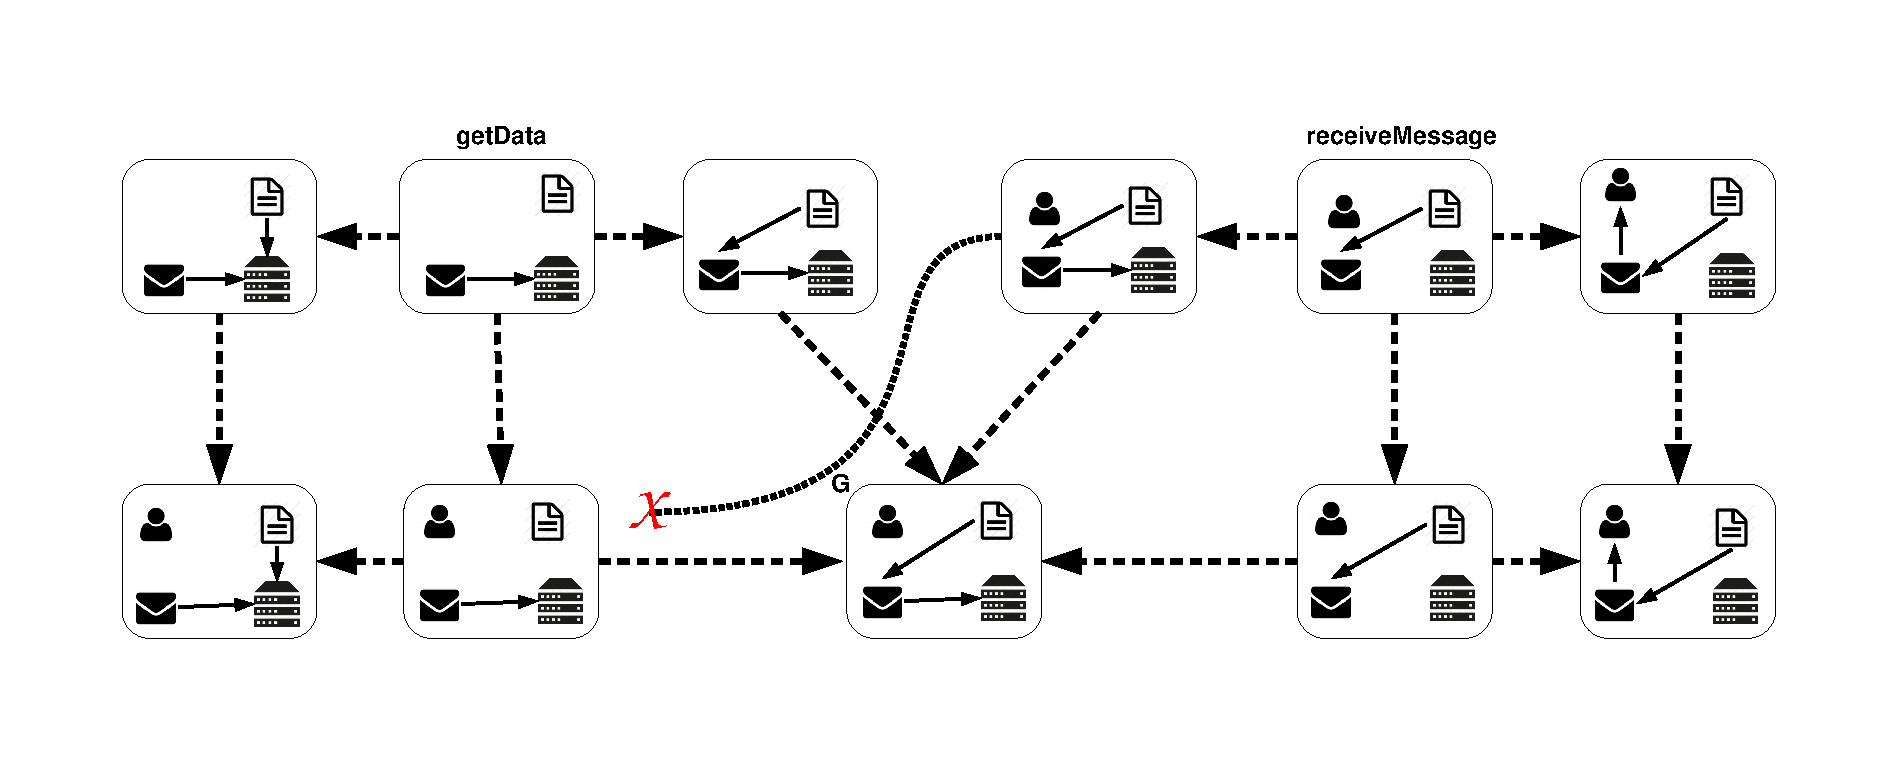
\includegraphics[scale=0.5]{images/gts/dependency}
  \caption{A dependency in the server grammar}\label{fig:gts:dependency}
\end{figure}

  In the diagram, it is not possible to find a morphism from the left-hand-side of \emph{receiveMessage} to the gluing graph of \emph{getData} such that the transformation is still valid. Thus, for the overlapping in this particular graph, \emph{receiveMessage} is causally dependent on \emph{getData}.
\end{example}

\begin{definition}[Conflict]\label{def:classic-conflict} Given two graph rules $p_1, p_2$ with NACs they are in conflict for a given graph $E$ in which they overlap iff one of the following situations occur:

\begin{enumerate}
    \item $\nexists h_{12} : L_1 -> D_2$ such that $d_2 \circ h_{12} = m_1$
    \item $\exists! h_{12} : R_1 -> D_2$ such that $d_2 \circ h_{12} = m_1$ but $e_2 \circ h_{12} \not\models NAC_{p_1}$
    \item $\nexists h_{21} : L_2 -> D_1$ such that $d_1 \circ h_{21} = m_2$
    \item $\exists! h_{21} : L_2 -> D_1$ such that $d_1 \circ h_{21} = m_2$ but $e_1 \circ h_{21} \not\models NAC_{p_2}$
  \end{enumerate}

\diagram{
     & & N_1 & & N_2 & & \\
      R_1\ar[d] & K_1\ar[d]\ar[l]\ar[r] & L_1\ar[u]^{n_1}\ar[dr]^{m_1}\ar@{.>}@/^1.1pc/[drrr]|<<{|}^<<<{h_{12}} & & L_2\ar[dl]_{m_2}\ar[u]^{n_2}\ar@{.>}@/_1.1pc/[dlll]|<<{|}_<<<{h_{21}} & K_2\ar[d]\ar[l]\ar[r] & R_2\ar[d]\\
        H_1 & D_1\ar[l]^{e_1}\ar[rr]_{d_1} & & \textit{E} & & D_2\ar[ll]^{d_2}\ar[r]_{e_2} & H_2\\
          & & & & & &
          }
\end{definition}

Intuitively, each conflict case can be regarded as:

\begin{enumerate}
  \item a \emph{delete-use} conflict: $p_2$ deletes (from graph $E$) at least one element needed for $p_1$ to be applied.
  \item a \emph{produce-forbid} conflict: $p_2$ produces (on graph $H_2$) at least one element that triggers the NAC $N_1$.
  \item a \emph{delete-use} conflict: $p_1$ deletes at least one element needed for $p_2$ to be applied
  \item a \emph{produce-forbid} conflict: $p_1$ creates at least one element that triggers the NAC $N_2$.
\end{enumerate}

\begin{example}[Conflict situation in the mail server grammar]
  Figure~\ref{fig:gts:dependency} shows a conflict situation involving the rules \emph{getData} and \emph{receiveMessage}. This is a \emph{delete-use} conflict: \emph{receiveMessage} deletes from the overlapping graph an edge between the \emph{message} and the \emph{server} which is necessary for \emph{getData} to be applied.

\begin{figure}[!ht]
  \centering
  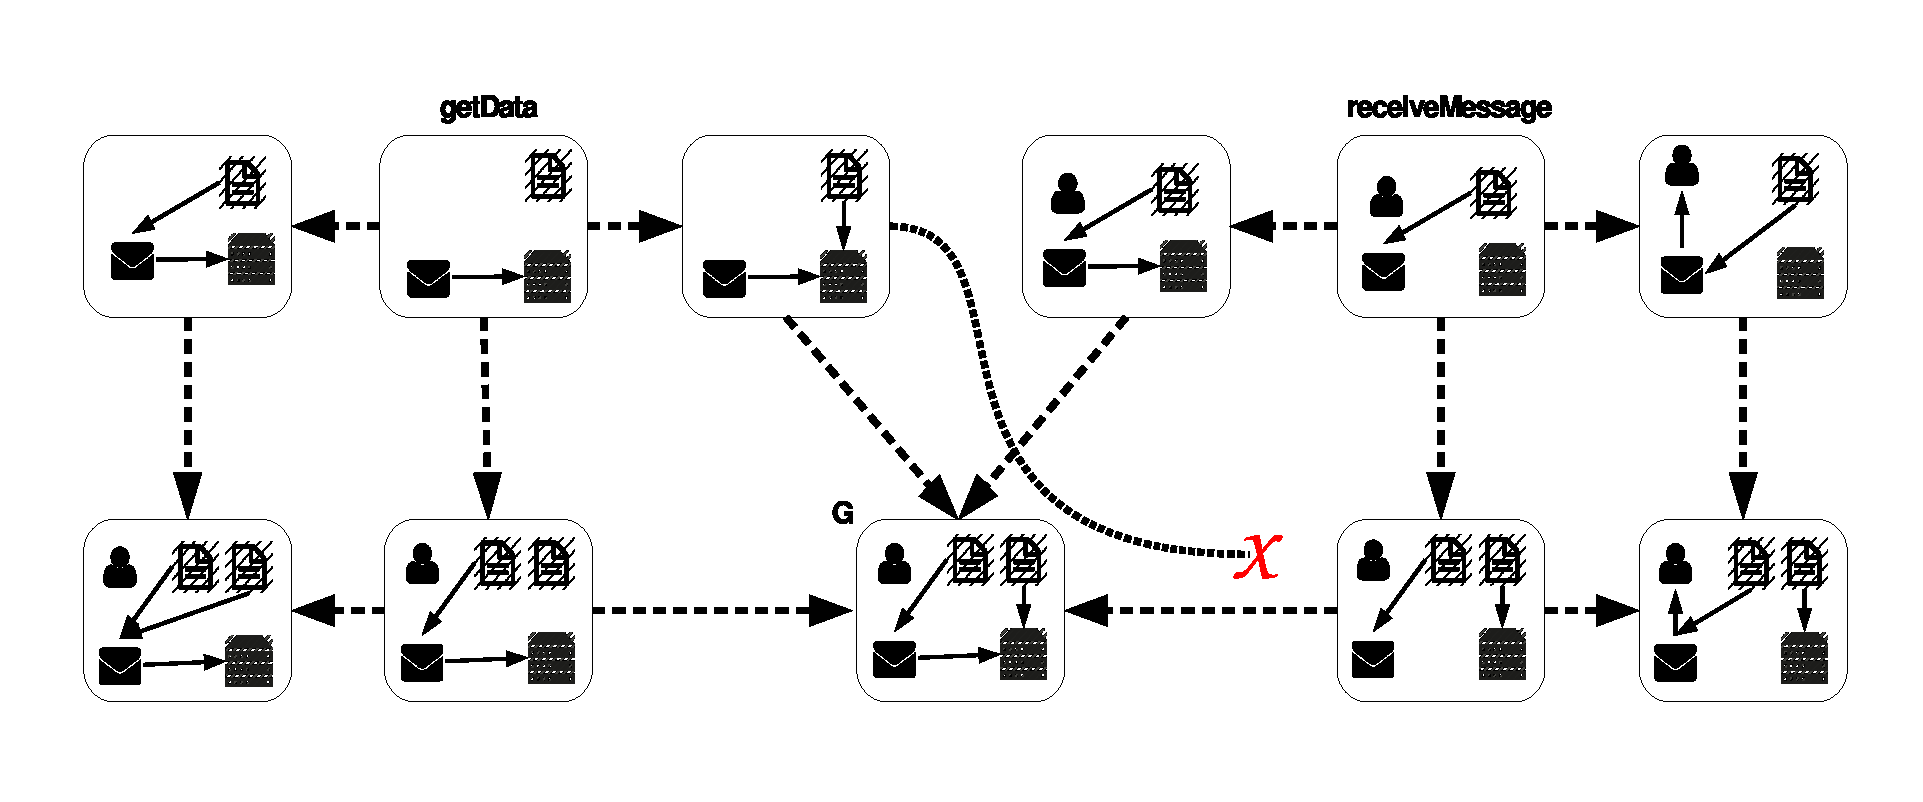
\includegraphics[scale=0.5]{images/gts/conflict}
  \caption{A conflict in the server grammar}\label{fig:gts:conflict}
\end{figure}

  Both rules are applied over the same graph and, individually, both transformations are valid. However, once \emph{receiveMessage} is applied, it is no longer possible to apply \emph{getData}. Represented in the diagram by the fat that it is not possible to find a morphism from the left-hand-side of \emph{getData} to the gluing graph of \emph{receiveMessage} such that the transformation from there is still valid.
\end{example}

%\chapter{Concurrent Rules}

\section{Motivation}

What kind of concurrent rule do we expect and why?

Used in ~\cite{BezerraWEIT2016} and implemented in ~\cite{BezerraETMF2016}

\textbf{From the paper}

Given its formalism, there are several analysis techniques that can be performed over a Graph Grammar, including the \emph{concurrent rule} construction, which can be used to summarize the application of a sequence of several rules in one single step.

Graph Grammars that represent real systems usually have a considerable number of rules, possibly making it difficult to the modeller to foresee all possible rule interactions. Therefore it is important to have analysis techniques to address this issue, as well as tools that implement them.

We said earlier that the aim of calculating the concurrent rules is to summarize the combined effects of applying the transformations induced by a sequence of graph rules. Here we present how this can be done.

A \emph{rule sequence} is a list containing rules of a grammar in an specific order in which the modeller wants them to be applied. Given a rule sequence \mbox{$r =$ \rulesequence}, the construction of its correspondents concurrent rules is done by recursively combining pairs of subsequent rules, where the pairwise combination is defined as follows~\cite{Ehrig2006,Lambers2010}:  

\section{Concurrent Rules}

\begin{definition}[Concurrent Rules]

\diagram{
  L_c\ar[d]\ar\ar@{}[dr]|{(3)} & K_c\ar[d]\ar[l]\ar[r] \ar@{}[dr]|{(1)} & R_c\ar[dr]^{e_1} & & L_n\ar[dl]_{e_2} & K_n\ar[d]\ar[l]\ar[r]\ar@{}[dl]|{(2)} & R_n\ar[d]\ar@{}[dl]|{(4)}\\
  L & C_c\ar[l]^{c_l}\ar[rr]_{c_r} & & \textit{E} & & C_n\ar[ll]^{n_l}\ar[r]_{n_r} & R\\
  & & & K\ar@{.>}@/1pc/[llu]^{k_c}\ar@{.>}@/1pc/[urr]_{k_n}\ar@{}[u]|{(5)} & & &
}
\end{definition}

\begin{definition}[Downward Shifted NACs]

\diagram{
  N'_j\ar@{.>}@/0.5pc/[r]^{e_{ji}} & N_i\ar@{}[dl]|{=}\\
  A\ar[r]_{m}\ar[u]^{n'_j} & B\ar[u]_{n_i}
}

For each $NAC(n'_j)$ on $A$ with $n'_j : A \rightarrow N'_j$ and $m : A \rightarrow B$, 
let $D_m(NAC(n'_j)) = \{ NAC(n_i)|i \in I, n_i : B \rightarrow N_i \}$ where $I$ and $n_i$ 
are constructed as follows:
\begin{itemize}
  \item $i \in I$ iff $(e_{ji}, n_i)$ with $e_{ji} : N'_j \rightarrow N_i$ jointly surjective 
  \item $e_{ji} \circ n_i = n_i \circ m$
  \item $e_{ji}$ injective
\end{itemize}

For each set of NACs $NAC_A = {NAC(N_j)| j \in J}$ on $A$ the downward shift of $NAC_A$ is then defined as: $D_m(NAC_A) = \cup_{j \in J}D_m(NAC(n'_j))$. $D_m$ is also called the \emph{Downward shift of $NAC_A$}.

\end{definition}

\begin{definition}[Left NACs from Right NACs]\label{def:shift-nac} To transfer a NAC over a rule or even over a span we can use de DPO rewriting, as in:\tinytodo{write the fundamentals of it}

\diagram{
  L\ar[d]_{n'_i} & K\ar[l]\ar[r]\ar[d] & R\ar[d]^{n_i}\\
  N'_i\ar@{}[ur]|{(2)} & D\ar[l]\ar[r] & N_i\ar@{}[ul]|{(1)}
}

\end{definition}

\begin{definition}[Concurrent Rules with NACs]

A concurrent rule is
\end{definition}

\centerline{
\xymatrix{
  N_i & & & & N_j & & \\
  L_c\ar[d]\ar[u]^{n_i}\ar@{}[dr]|{(3)} & K_c\ar[d]\ar[l]\ar[r] \ar@{}[dr]|{(1)} & R_c\ar[dr]^{e_1} & & L_n\ar[dl]_{e_2}\ar[u]^{n_j} & K_n\ar[d]\ar[l]\ar[r]\ar@{}[dl]|{(2)} & R_n\ar[d]\ar@{}[dl]|{(4)}\\
  L & C_c\ar[l]^{c_l}\ar[rr]_{c_r} & & \textit{E} & & C_n\ar[ll]^{n_l}\ar[r]_{n_r} & R\\
  & & & K\ar@{.>}@/1pc/[llu]^{k_c}\ar@{.>}@/1pc/[urr]_{k_n}\ar@{}[u]|{(5)} & & &
}}

\begin{itemize}
\item $n = 0$ The \emph{concurrent rule} $p_c$ with NACs for rule $p_0$ with NACs is $p_0$ with NACs itself.
\item $n \geqslant 1$ A concurrent rule $p_c = p'_c \ast_E p_n $ with NACs for the rule sequence \rulesequence is defined recursively as $p_c = (l_c \circ k_c : K \rightarrow L, r_n \circ k_n : K \rightarrow R)$ where 
  \begin{itemize}
  \item $p'_c : L'_c \leftarrow K'_c \rightarrow R'_c$ is a concurrent rule for the sequence $p_0,\ldots,p_{n-1}$
  \item $(e'_c,e_n)$ is jointly surjective
  \item (1), (2), (3) and (4) are pushouts
  \item (5) is a pullback
  \item $N_i$ is shifted over morphism $l'$
  \item $N_j$ is shifted over morphism $e_2$ and then over the ``rule'' $q'_c = l_c : C_c \rightarrow L, r_c : C_c \rightarrow E$
  \end{itemize}
\end{itemize}

\begin{definition}[Concurrent Rules induced by Dependencies]

  \textbf{incomplete}

  The default algorithm constructs the concurrent rules based on all the overlappings of the right side of the first rule and left side of the second rule, allowing us to see how the elements created/preserved by one rule can be connected with the elements deleted/preserved by the other.

  One way to restrict the number of possible concurrent rules and still generate meaningful rules is to filter and use only the overlappings associated with dependencies~\cite{Lambers2006} between subsequent pairs of rules. The idea behind this is to use only the overlappings where (1) the elements needed for the second rule to be applied are explicitly created by the first one or (2) the elements forbidden by the NACs of the second rule are explicitly deleted by the first.

  For the first case, we only need to filter the overlappings in the concurrent rule diagram where $\nexists h_{12} : R'_c \rightarrow C_n$ such that $(l_n \circ h_{12} = e_1$ and $r_n \circ h_{12} \models N^{-1}_i)$ or $\nexists h_{21} : L_n \rightarrow C_c$ such that $(r_c \circ h_{21} = e_2$ and $l_c \circ h_{21} \models N_j)$.

  However, this notion does not take into consideration the elements whose existence is forbidden by the NACs of the second rule and would then forbid its application, but once deleted by the first rule the application of the second is enabled.

  We did not find on the literature a construction to capture those cases, however an adaptation of the concurrent rule algorithm can be made based on the algorithm for calculating dependencies between the rules defined in~\cite{Lambers2006}. Besides the overlappings between $(R'_c, L_n)$ that represent dependencies, we generate \emph{also} the overlappings of the left side of the first rule $L'_c$ with the NACs $N_j$ and check whether the rewritings are possible, in which case the
  diagram for the corresponding concurrent rule construction can be seen as follows:

\diagram{
  N_i& & & & N_j\ar@{.>}@/_3pc/[ddllll]_{e_2} & & \\
  L_c\ar[u]^{n_i}\ar[d]_{e_1}\ar@{}[dr]|{(1)} & K_c\ar[d]\ar[l]\ar[r] \ar@{}[dr]|{(2)} & R_c\ar[dr]^{m'_1} & & L_n\ar[dl]_{m_2}\ar[u]^{n_j} & K_n\ar[d]\ar[l]\ar[r]\ar@{}[dl]|{(3)} & R_n\ar[d]^{m'_2}\ar@{}[dl]|{(4)}\\
  \textit{E} & C_c\ar[l]|{c_l}\ar[rr]|{c_r} & & P_1 & & C_n\ar[ll]|{n_l}\ar[r]|{n_r} & P_2\\
  & & & K\ar@{.>}@/1pc/[llu]|{k_c}\ar@{.>}@/1pc/[urr]|{k_n}\ar@{}[u]|{(5)} & & & 
}

\end{definition}
% \ar@{.>}@/_1pc/[dlll]|{X_{h_{21}}}

\begin{thm}[EpiPairs]
  \begin{proof}{Incomplete}
  \end{proof}
\end{thm}

\section{Dealing with the combinatorial explosion}\label{sec:explosion}

There exist some strategies that can help dealing with the combinatorial explosion of by addressing some specificities of the problem domain. The strategies explained in the following do not solve the theoretical worst cases, but they have been showed to be good enough in most of our practical cases.

\subsection{Trivially-triggered NACs}

For each pair of rules $(p_c,p_n)$ for which we want to generate the corresponding concurrent rules, we must first generate all possible overlappings between $R_c$ and $L_n$, check whether they satisfy the gluing conditions and calculate the pushouts and pullbacks that will result in the concurrent rules. However, it is possible that some of the generated overlappings result in epimorphic pairs $(E, e_1 : R_c \rightarrow E, e_2 : L_n \rightarrow E)$ whose morphisms $e_1$ or $e_2$ do not satisfy
the right NACs of $p_c$ or the left NACs of $p_n$, respectively.

In such cases, the NACs forbid the existence of valid transformations \mbox{$L \xRightarrow{p_c,l'} E$} and $E \xRightarrow{p_n,r'} R$ even though the gluing conditions are satisfied. It means that the rules could not be applied over the graph $E$. We may them ignore such overlappings when calculating possible concurrent rules.

If we do maintain those pairs for computation, as the shift of NACs aims to translate the NACs of each rule to sets of equivalent NACs in the concurrent rules, we would generate rules where for every possible match of $L$, there will always be a NAC not satisfied by $m$, thus the rule would never be applicable.

\begin{thm}[Propagation of trivially triggered NACs over concurrent rules]
  \begin{proof}{Yet to come}
  \end{proof}
\end{thm}

\subsection{Graph Constraints}\label{sec:constraints}

Graph constraints can be used to globally enforce or prohibit the existence of certain structures in the graphs that can be generated by a graph grammar. For example, they can be used to define minimal and maximal multiplicities for nodes and edges.

When calculating the concurrent rules for a pair $(p_c, p_n)$ we first use them similarly to the use of NACs, checking whether the generated overlappings satisfy the graph constraints, cutting off those who do not, which can also lead to a reduction of possible concurrent rules. Fig~\ref{fig:constraints} shows two negative atomic constraints that (a) forbid the existence of more than one server and (b) forbid a piece of data of being in two different messages at the same time. Look at
Fig~\ref{fig:epipairs} again to see that two of the overlappings would be cut off by these constraints.

We can still use the graph constraints to cut off even more concurrent rule candidates, because even though the overlappings satisfy the gluing conditions and NACs, the resulting $lhs$ and $rhs$ may still not satisfy the graph constraints. 

When dealing with injective morphisms, if a graph $L$ of a rule does not satisfy the graph constraints, no possible \match{} can be found in which $G$ satisfies the constraints, thus the rule can never be applied and we can discard it. Similar reasoning can be applied to the $R$ graph and \comatch{}.

\begin{figure}
\centering
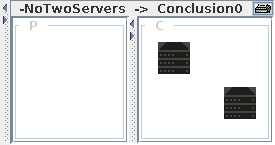
\includegraphics{grammar/no_two_servers}
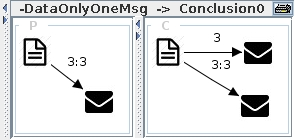
\includegraphics{grammar/data_no_two_msgs}
\caption{\label{fig:constraints} Negative atomic constraints for server}
\end{figure}

\subsection{Concurrent Rules Induced by Dependencies}

The default algorithm constructs the concurrent rules based on all the overlappings of the right side of the first rule and left side of the second rule, allowing us to see how the elements created/preserved by one rule can be connected with the elements deleted/preserved by the other.

One way to restrict the number of possible concurrent rules and still generate meaningful rules is to filter and use only the overlappings associated with dependencies~\cite{Lambers2006} between subsequent pairs of rules. The idea behind this is to use only the overlappings where (1) the elements needed for the second rule to be applied are explicitly created by the first one or (2) the elements forbidden by the NACs of the second rule are explicitly deleted by the first.

For the first case, we only need to filter the overlappings in the concurrent rule diagram where $\nexists h_{12} : R'_c \rightarrow C_n$ such that $(l_n \circ h_{12} = e_1$ and $r_n \circ h_{12} \models N^{-1}_i)$ or $\nexists h_{21} : L_n \rightarrow C_c$ such that $(r_c \circ h_{21} = e_2$ and $l_c \circ h_{21} \models N_j)$.

However, this notion does not take into consideration the elements whose existence is forbidden by the NACs of the second rule and would then forbid its application, but once deleted by the first rule the application of the second is enabled.

We did not find on the literature a construction to capture those cases, however an adaptation of the concurrent rule algorithm can be made based on the algorithm for calculating dependencies between the rules defined in~\cite{Lambers2006}. Besides the overlappings between $(R'_c, L_n)$ that represent dependencies, we generate \emph{also} the overlappings of the left side of the first rule $L'_c$ with the NACs $N_j$ and check whether the rewritings are possible, in which case the
diagram for the corresponding concurrent rule construction can be seen as follows:

\diagram{
    N_i& & & & N_j\ar@{.>}@/_3pc/[ddllll]_{e_2} & & \\
      L'_c\ar[u]^{n_i}\ar[d]_{e_1}\ar@{}[dr]|{(1)} & K'_c\ar[d]\ar[l]\ar[r] \ar@{}[dr]|{(2)} & R'_c\ar[dr]^{m'_1} & & L_n\ar[dl]_{m_2}\ar[u]^{n_j} & K_n\ar[d]\ar[l]\ar[r]\ar@{}[dl]|{(3)} & R_n\ar[d]^{m'_2}\ar@{}[dl]|{(4)}\\
        \textit{E} & C_c\ar[l]|{c_l}\ar[rr]|{c_r} & & P_1 & & C_n\ar[ll]|{n_l}\ar[r]|{n_r} & P_2\\
          & & & K\ar@{.>}@/1pc/[llu]|{k_c}\ar@{.>}@/1pc/[urr]|{k_n}\ar@{}[u]|{(5)} & & & 
          }\vspace{-15pt}


          \subsection{Maximal Concurrent Rule}

          Sometimes, instead of generating all possible overlappings or even all the dependencies, the modeller is interested in seeing only the maximal interactions between the elements of each rule in the sequence, thus we may filter the overlappings with the least number of elements, capturing the cases where the elements of each rule are as connected as possible. Note that the rule in Fig~\ref{fig:concurrent_rule_construction} is a maximal concurrent rule.


\section{Comparison or Results}

\chapter{Occurrence Graph Grammars}\label{ch:process}

Occurrence graph grammars were defined by~\cite{Ribeiro1996} for the SPO approach and by~\cite{Corradini1996} for the DPO approach as a formalism for representing the concurrent semantics of a graph grammar which is still a graph grammar. Thus it is possible to use occurrence graph grammars to describe all possible states and changes of states of the original graph grammars from where they are generated. 

They also contain the entire execution history of the original grammar in the form of (1) a \emph{core graph} that contains all the elements that ever existed in the execution of the grammar and (2) a set of \emph{relations} between the elements of this core graph, which can tell us properties about the existence of those elements: which of them must occur at the same state, which must occur one after the other, which elements must never occur together, and so on.

These properties make occurrence graph grammars a good candidate for the generation of test cases, as we are interested in a way of representing several (equivalent) possible derivations in a compact notation for later generation of tests.

However, the first definitions of occurrence graph grammar do not use negative application conditions, which are nowadays essential to the modelling of complex systems as graph grammars as they provide more possibilities to control the application of rules~\cite{Lambers2008, Corradini2014}.

This chapter extends the works of~\cite{Ribeiro1996} and~\cite{Corradini1996}, by reviewing what occurrence graph grammars are and then extending them to include negative application conditions.

\section{Doubly-Typed Graph Grammars}

\begin{definition}[Doubly-Typed Graph] Given a type graph $T$, a \emph{doubly-typed graph} \doublyTypedGraph{} over $T$ is a tuple \doublyTypedGraph $= \left(G^T,TG^T, t^{G^T} : G^T \rightarrow TG^T\right)$ where $G^T$ and $TG^T$ are typed graphs over $T$ and \mbox{$t^{G^T} : G^T \rightarrow TG^T$} is a typed graph morphism in \typedGraphCategory{}. We call $TG^T$ the \emph{double-type graph} and $t^{G^T}$ the double-typing morphism.
\end{definition}

\begin{remark}[Typing Morphism] In this work, we will consider only doubly-typed graphs whose typing morphism $type_{TG} : TG \rightarrow T$ is an epimorphism. This has the effect that every element present in $T$ is mapped by at least one element from $TG$.
\end{remark}

\begin{example}[Doubly-Typed Graph Example] Figure~\ref{fig:process:doubly-typed-graph} shows a doubly-typed graph $G^{TG^T}$.

\begin{figure}[!ht]
  \centering
  \fbox{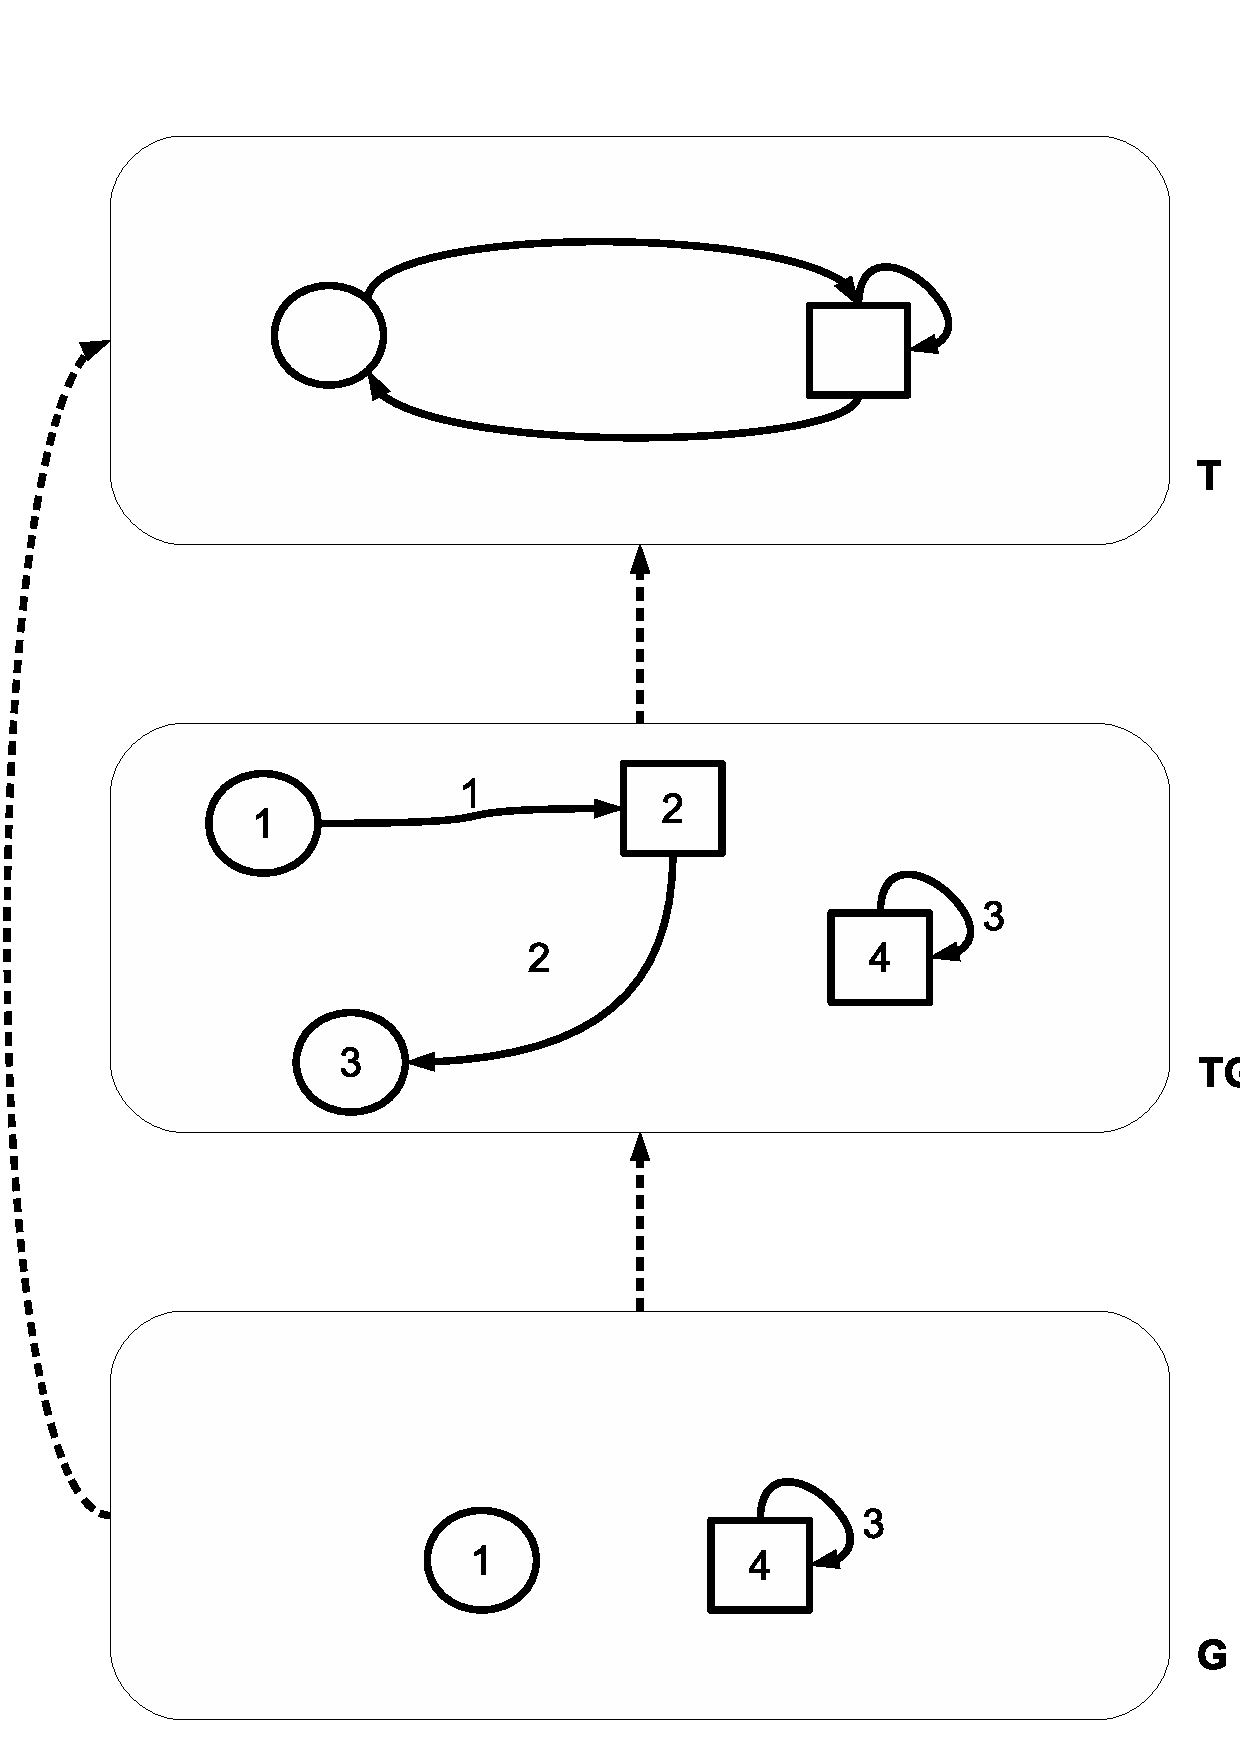
\includegraphics[scale=0.4]{images/process/doubly-typed-graph-example}}
  \caption{Doubly-typed graph}\label{fig:process:doubly-typed-graph}
\end{figure}

\end{example}

\begin{definition}[Doubly-Typed Graph Morphism]
  Given two doubly-typed graphs $G^{TG^T}$ and $H^{TG^T}$ and a graph morphism $g^T : G^T \rightarrow H^T$, we say that $g^T$ is a \emph{$TG^T$-doubly-typed graph morphism} if the following diagram commutes:

\diagram{
  G\ar[rr]^{g}\ar[dr]_{t^{G}}& & H\ar[dl]^{t^{H}} \\
   & TG\ar[d]^{type_{TG}} & \\
  & T &
}
\end{definition}

Notice that the (single) type morphisms $type_G : G \rightarrow T$ and $type_H : H \rightarrow T$ can be obtained respectively as $type_{TG} \circ t^G$ and $type_{TG} \circ t^H$.

\begin{example}[Doubly-Typed Graph Morphism Example] Figure~\ref{fig:process:doubly-typed-graph-morphism} shows a doubly-typed graph morphism $f : G^{TG^T} \rightarrow H^{TG^T}$.

\begin{figure}[!ht]
  \centering
  \fbox{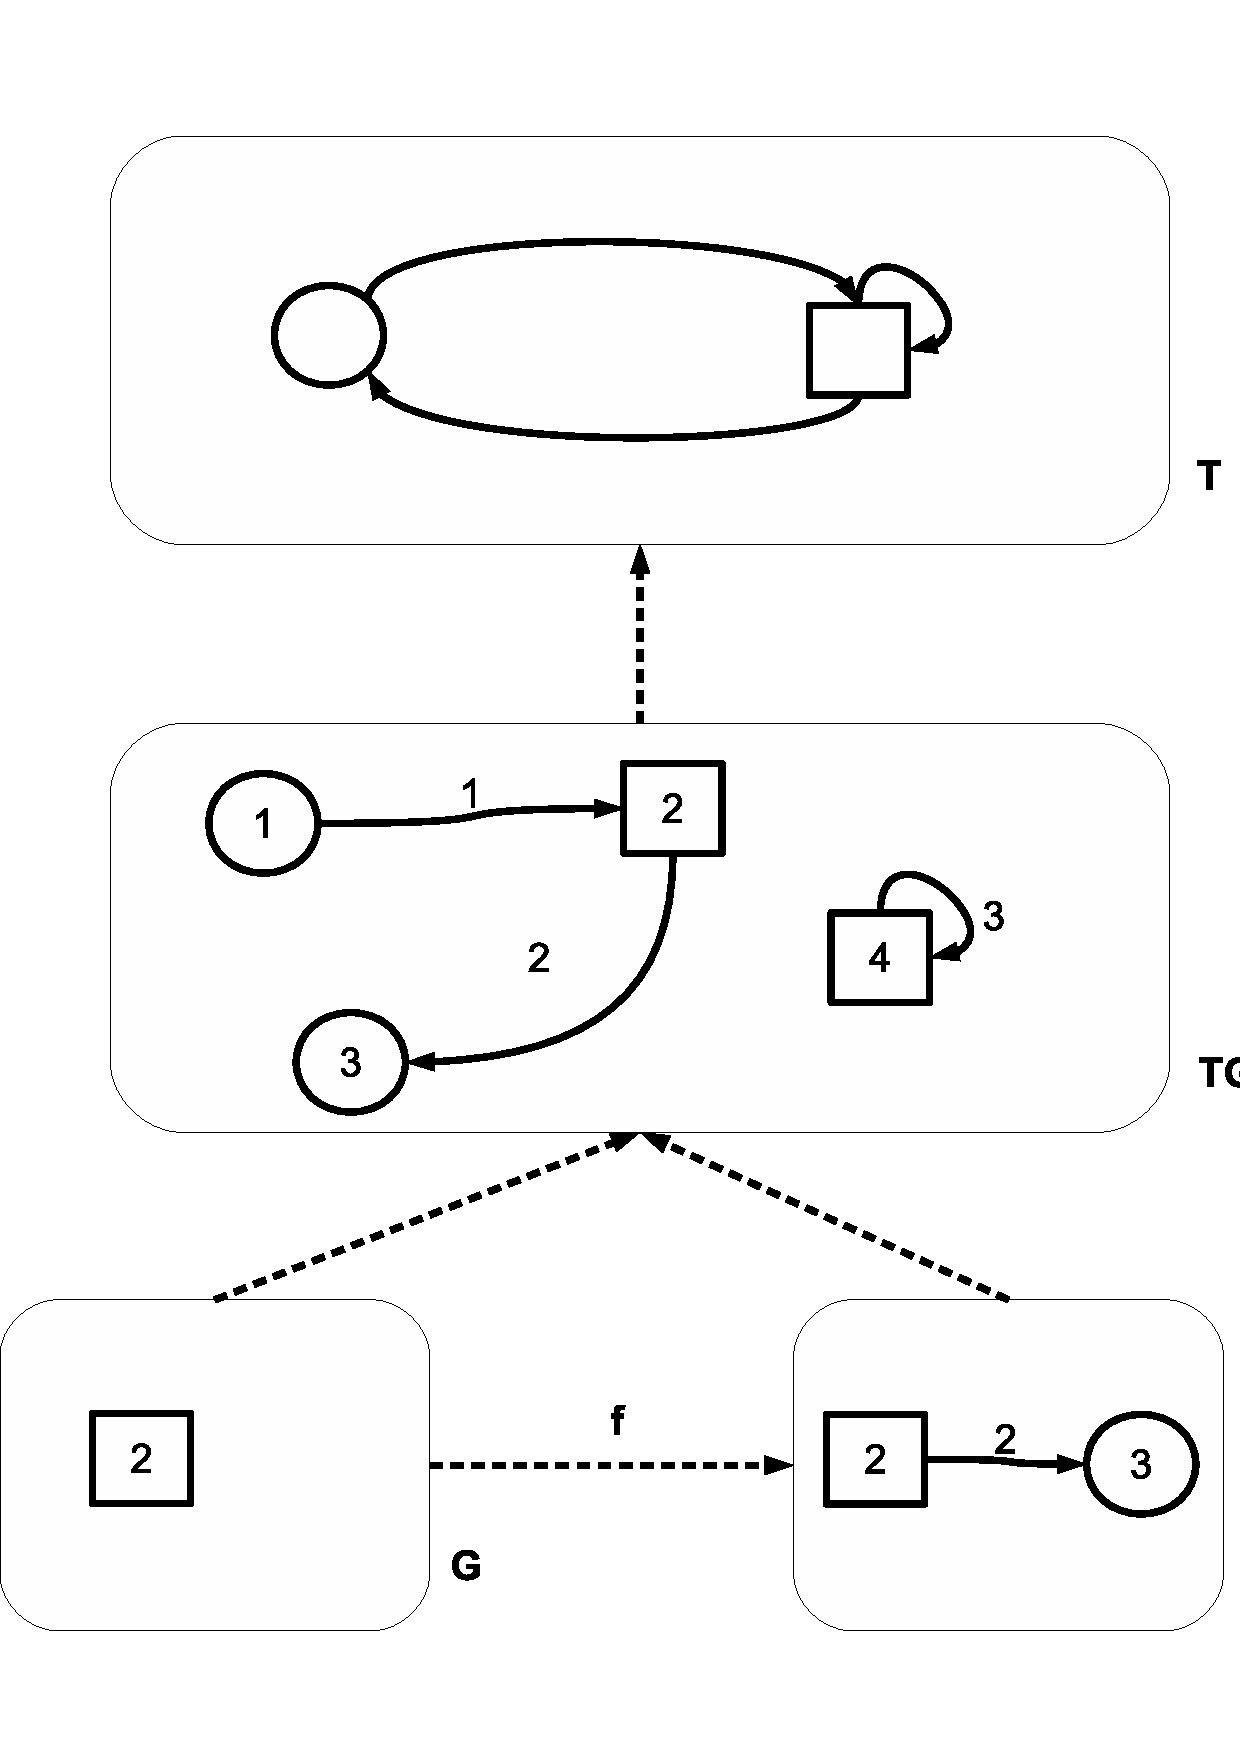
\includegraphics[scale=0.4]{images/process/doubly-typed-graph-morphism-example}}
  \caption{Doubly-typed graph morphism}\label{fig:process:doubly-typed-graph-morphism}
\end{figure}
\end{example}

\begin{remark} There could be defined different kinds of doubly-typed graph morphisms depending on whether the doubly-type graphs and the type graphs are or not the same. However, we are here only interested in the case where all doubly-typed graphs share the same double-type and type graphs.

Therefore we will call \mbox{\emph{$TG^T$-doubly-typed graph morphisms}} simply by \emph{doubly-typed graph morphisms} through the rest of this work.

\end{remark}


\begin{definition}[Doubly-Typed Graph Rule] A doubly-typed graph rule \doublyTypedRule{} is a span of injective doubly-typed graph morphisms $l : K \rightarrow L$ and $r : K \rightarrow R$.

\diagram{
  L\ar[dr] & K\ar[l]\ar[r]\ar[d] & R\ar[dl]\\
    & TG\ar[d] & \\
    & T &
}

  Given a doubly-typed graph rule \doublyTypedRule{}, its inverse rule is defined by \inverseDoublyTypedRule{}.

  Let the double-typing morphisms from $L^{TG^T}$, $K^{TG^T}$ and $R^{TG^T}$ be $t^{L^T}$, $t^{K^T}$ and $t^{R^T}$, respectively. For a rule $a = p^{TG^T}$ we call:

  \begin{itemize}
    \item $L_a = L_T$, $K_a = K_R$ and $R_a = R_T$, the left, gluing and right graphs of $a$.
    \item $pre_a = t^{L^T} : L^T \rightarrow TG^T$, the \emph{pre-condition} of the $a$.
    \item $post_a = t^{R^T} : R^T \rightarrow TG^T$, the \emph{post-condition} of $a$.
    %\item $r_a = r^T$, the \emph{rule pattern} of $a$.\tinytodo{Not sure if we will need the rule pattern.}
  \end{itemize}

\end{definition}

\begin{example}[Doubly-Typed Graph Rule Example]Figure~\ref{fig:process:doubly-typed-graph-rule} shows a doubly-typed graph rule which deletes an edge $\curvearrowleft_1$ and a node $\Circle_1$, preserves a $\Square_2$ and creates a node $\Circle_3$ and an edge $\curvearrowleft_2$.

\begin{figure}[!ht]
  \centering
  \fbox{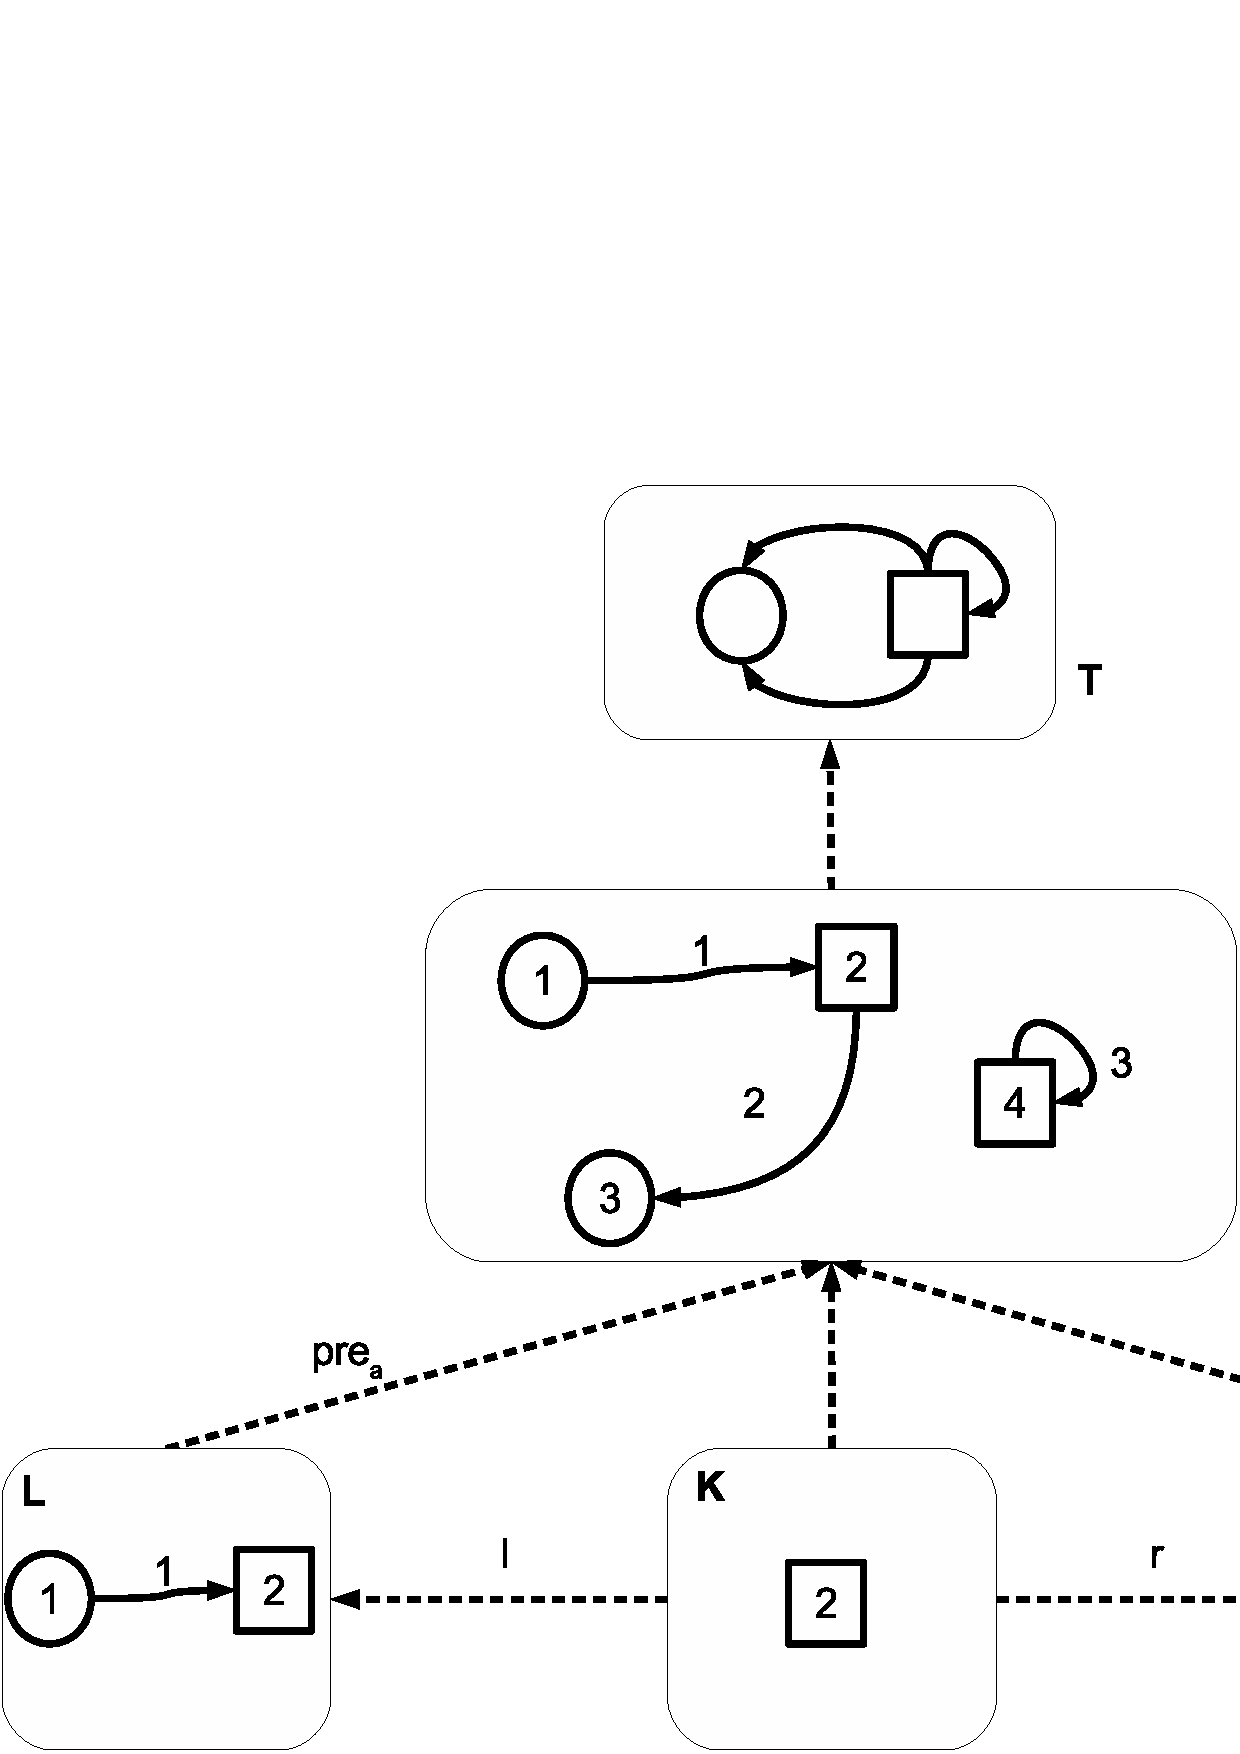
\includegraphics[scale=0.5]{images/process/doubly-typed-graph-rule-example}}
  \caption{Doubly-typed graph rule}\label{fig:process:doubly-typed-graph-rule}
\end{figure}
\end{example}

\begin{definition}[Negative Application Conditions on Doubly-Typed Graph Rules] A \emph{left} negative application condition over a doubly-typed graph rule $p^{TG^T}$ is of the form $NAC(n^T)$, where $n^T : L^T \rightarrow N^T$ is an arbitrary (single-)typed graph morphism. 
 
A (doubly-typed) match morphism $m^{TG^T} : L^{TG^T} \rightarrow G^{TG^T}$ of a rule $p^{TG^T}$ satisfies $NAC(n^T)$ on $L^{TG^T}$, written \mbox{$m^T \models NAC(n^T)$}, iff $\nexists$ $q^T : N^T \rightarrow G^T$ where $q^T$ injective and $q^T \circ n^T = m^T$.

\diagram{
  T & TG\ar[l]\\
  N\ar[u]\ar@{.>}[dr]|{|}_{q} & L\ar[u]\ar[d]^{m}\ar[l]_{n}\\
   & G\ar@/_2.1pc/[uu]
}

  A match $m^{TG^T} : L^{TG^T} \rightarrow G^{TG^T}$ satisfies a set \mbox{$NAC_L = \{NAC\left(n^T_i\right)|i \in I\}$} of left $NACs$, iff \mbox{$m \models NAC\left(n^T_i\right)$} $\forall i \in I$.

\emph{Right} negative application conditions are defined analogously for the right hand side of a rule and its comatch.


\end{definition}

\begin{example}[NAC Example]
\end{example}

\begin{remark}
Although we could have defined NACs whose morphisms are doubly-typed graph morphisms (which would then act specifically over doubly-typed graphs) we will not use this kind of NACs later in our work. Therefore, we will use this \emph{single-typed} NACs as the only NAC type in all of our \emph{doubly-typed graph grammars}, and $NAC(n)$ as a synonym of $NAC(n^T)$.
\end{remark}

When dealing with the classical notion of NACs, there may occur situations where the NAC of a rule can be triggered by the cumulative effect of applying two (or more) other rules, while the same rules would not trigger this NAC without the other. This may lead to a situation where conflicts and dependencies are not stable under switch, as shown in example~\ref{ex:process:instability}.

\begin{example}[Instability of Conflicts and Dependencies]\label{ex:process:instability}The rules depicted in Figure~\ref{fig:process:instability} show a situation where the independency between rules is not stable under switch equivalence.

  In this example, all rules are independent and also do not conflict with each other in the sense of Definitions~\ref{def:classic-dependency} and~\ref{def:classic-conflict}. Thus, in theory, it should be possible to apply this rules in any order or in parallel. Particularly, it is possible to apply all rules in the order they appear in the figure, i.e. $[p_1, p_2, p_3]$.

  It is also possible to apply them in the orders $[p_1, p_3, p_2]$, $[p_2, p_1, p_3]$ and $[p_3, p_1, p_2]$. However, we can no longer apply all rules if we use the sequences $[p_2, p_3, p_1]$ or $[p_3, p_2, p_1]$.

  This problem arises from the fact that $p_2$ and $p_3$ independently create a piece of the pattern forbidden by the NAC of $p_1$. In a way that, although the effects of each rule by themselves do not trigger the NAC of $p_1$, their combined effects do.

\begin{figure}[!ht]
  \centering
  \fbox{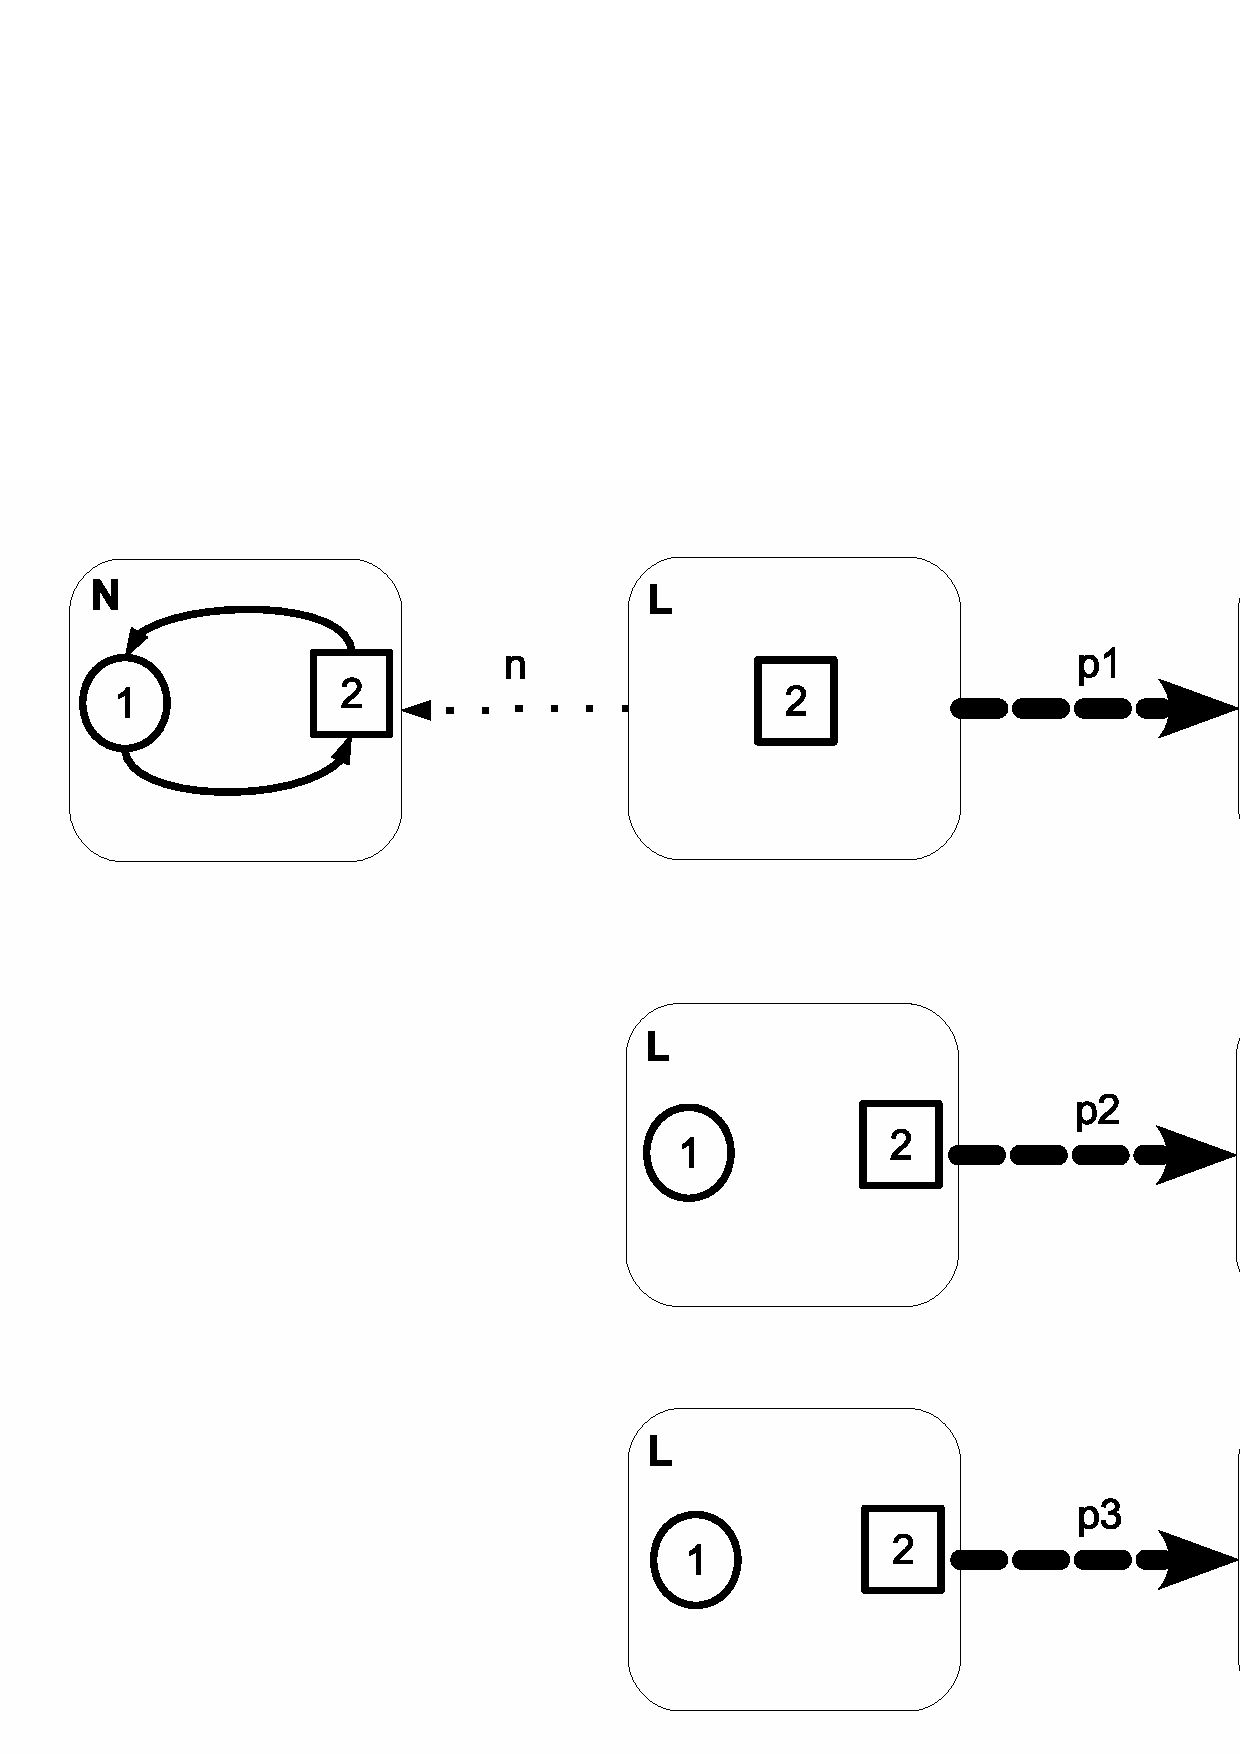
\includegraphics[scale=0.4]{images/process/instability-example}}
  \caption{Instability of conflicts under shift\\}\label{fig:process:instability}
\end{figure}

\end{example}

As we are interested in constructing a canonical representation of several possible derivations for a set of rules in a grammar, we will make use of a special type of NACs called \emph{incremental NACs} that aim to address this issue.

\emph{Incremental NACs}, originally defined in~\cite{Corradini2013} and~\cite{Corradini2014}, have the property of extending the forbidden context of a match by a single edge or a single node. This can be regarded as each NAC forbidding only one element at a time, thus there is no possible way to trigger a NAC by the cumulative effect of more than one rule.


\begin{definition}[Incremental NACs] Given a monomorphism \mbox{$n : L \rightarrow N$}, $NAC(n)$ is said to be incremental if for any possible pair of decompositions \mbox{$g_1 : L \rightarrow O_g;g_2 : O_g \rightarrow N$} and \mbox{$f_1 : L \rightarrow O_f;f_2 : O_f \rightarrow N$} as in the diagram below, where all morphisms are monos and \mbox{$f_1;f_2 = n = g_1;g_2$}, there exists a mediating morphism $o_1 : O_g \rightarrow O_f$ or $o_2 : O_f \rightarrow O_g$, such that the resulting triangles
  commutes.

\diagram{
  & O_g\ar[dr]^{g_2}\ar@{.>}@/_0.5pc/[dd]|<<<<<<{o_1} &  \\
  L\ar[ur]^{g_1}\ar[dr]_{f_1}\ar[rr]|<<<<{n}&     & N\\
    & O_f\ar[ur]_{f_2}\ar@{.>}@/_0.5pc/[uu]|<<<<<<<<{o_2} & 
}

\end{definition}

\begin{example}[Incremental NACs]Figure~\ref{fig:process:incremental-nacs} shows all possible formats that any valid incremental NAC can assume.

\begin{figure}[!ht]
  \centering
  \fbox{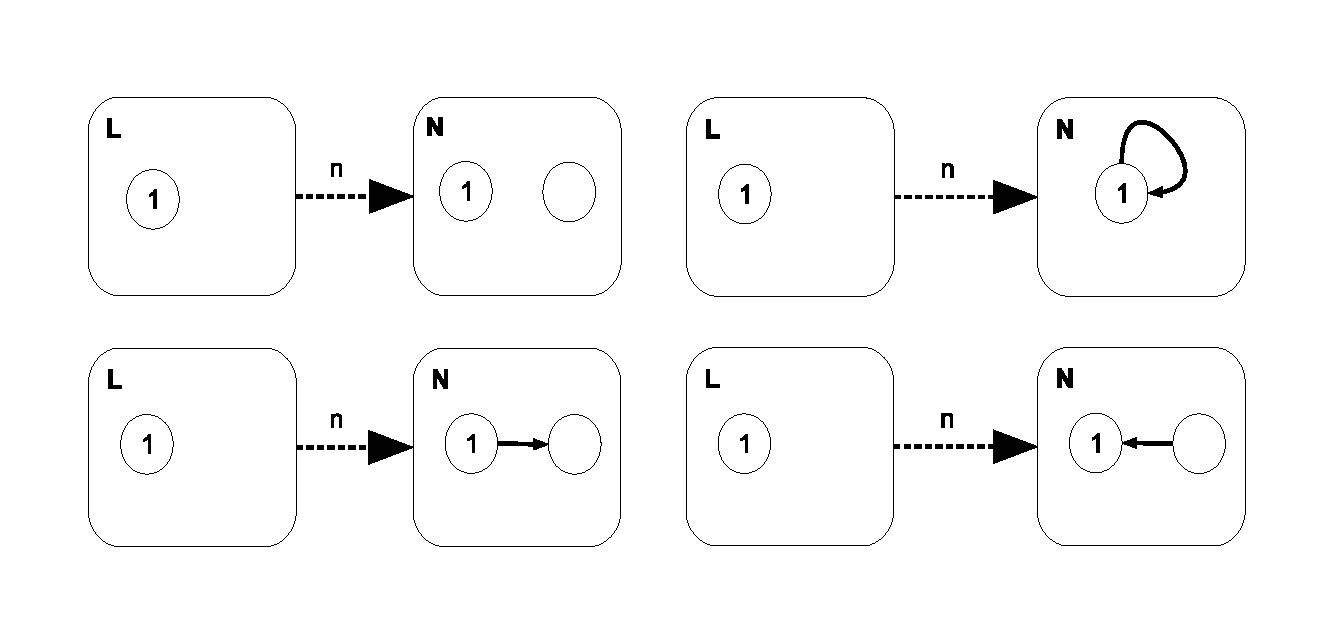
\includegraphics[scale=0.65]{images/process/incremental-nacs}}
  \caption{Incremental NACs possible formats}\label{fig:process:incremental-nacs}
\end{figure}
\end{example}

At first, it may seem that we are loosing expressive power by restricting the NACs we use in our grammars to incremental NACs only, however ~\cite{Corradini2013} has shown two important results regarding that.

First, they show that incremental NACs are sufficient to model most of real applications using $GTSs$. Second, they present an algorithm to compile rules with general NACs to rules with incremental NACs only, generating a new $GTS$ that is able to simulate the old one.

Despite of it, the implementation of the compiling algorithm is out of the scope of this thesis and it is left as future work.

\begin{definition}[Triggering element] Given a rule \graphrule{} with an incremental, non trivially triggered NAC \nac{}, and a monomorphic match \match{}, where there is an injective $q : N \rightarrow G$, therefore $m \not\models NAC(n)$. We have that the element that will complete the match towards triggering the NAC is present in the difference between the images of $q$ and $m$.

  Let $G_{|N}$ be the image of $q$ and $G_{|L}$ the image of $m$, and \mbox{$T = G_{|N} - G_{|L}$}.\footnote{In this case, $T$ may not be a graph, we are here abusing the notation and treating $T$ as a set $V$ of vertices and a set $E$ of edges.} The triggering element of this NAC is:

  \begin{itemize}
    \item $x \in E(T)$, if $E(T) \neq \varnothing$;
    \item $x \in V(T)$ otherwise.
  \end{itemize} 
\end{definition}

\begin{example}[Triggering Element]
Since incremental NACs extend the match by forbidding only one element at a time, this element can be easily identified when looking at the instance graph.\tinytodo{Prepare example}
\end{example}

\begin{definition}[Doubly-Typed Graph Grammars] A \emph{doubly-typed graph grammar} is a tuple $GG = \left(TG^T, I^{TG^T},P \right)$ where $TG^T$ is the double-type graph of the grammar, $I^{TG^T}$ is a doubly-typed graph, called the \emph{initial graph} of the grammar and $P$ is a set of doubly-typed graph rules.
\end{definition}

\begin{definition}[Core Graph]\label{def:core-graph} Given a doubly-typed graph grammar \doublyTypedGraphGrammarCore{}, we have that \coreGraph{} is a \emph{core graph} iff the following two conditions hold:

\begin{enumerate}

\item \mbox{$\forall x \in$ \coreGraph $: \exists! y \in (I^T \uplus (\uplus_{i \in P} (R_i - K_i))$}:
\[ x =
    \begin{cases}
      in_{GG}\parens{y},$ if $y \in I^T\\
      post_i(y),$ if $y \in R_i - K_i\\
    \end{cases}
   \]

\item \mbox{$\forall x \in$ \coreGraph $: \exists^{\leq1} y \in \uplus_{i \in P} (L_i - K_i)$}:
\[ x =
    \begin{cases}
      pre_i(y),$ if $y \in L_i - K_i\\
    \end{cases}
   \]\end{enumerate}

  The first condition assures that every element in the \emph{core graph} was either already present in the initial graph or was created by one and only rule. The second condition assures that for every element that is deleted, it is deleted only once by only one rule.
\end{definition}

The idea is that each element within a \emph{core graph} has a unique origin. At the same time, the \emph{core graph} contains all elements necessary (created, deleted and preserved) by all rules in its underlying grammar.

\begin{example}[Doubly-Typed Graph Grammar and Core Graph Example] \mbox{Figure~\ref{fig:process:core-graph:counter-example}} shows a doubly-typed graph grammar, whose double-type is not a core graph. That happens because $\Square_2$ is created by both rules $p_1$ and $p_2$, as well as $\Circle_1$ is deleted by both $p_2$ and $p_3$.

  On the other hand, Figure~\ref{fig:process:core-graph:example} shows a doubly-typed graph grammar whose double-type is also a core graph: all elements are either created only once or, if not created by any rule, are present in the initial graph: $\Square_2$ and $\curvearrowleft_1$ are created by $p_1$, $\curvearrowleft_3$ by $p_2$, $\Circle_3$ and $\curvearrowleft_2$ by $p_3$ and $\Circle_1$ is present on the initial graph. Also, the deleted elements are deleted only once: $\Circle_1$ and
  $\curvearrowleft_1$ by $p_3$.

  It is important to notice that, even though the $TG$ graphs in both grammars are isomorphic, only the one in Figure~\ref{fig:process:core-graph:example} is a core graph. This can be explained by looking to their underlying grammars (initial graphs and rules), where one of them satisfies the conditions presented in Definition~\ref{def:core-graph} and the other not.
\begin{figure}[!ht]
  \centering
  \begin{subfigure}[t]{.5\textwidth}
    \centerline{\fbox{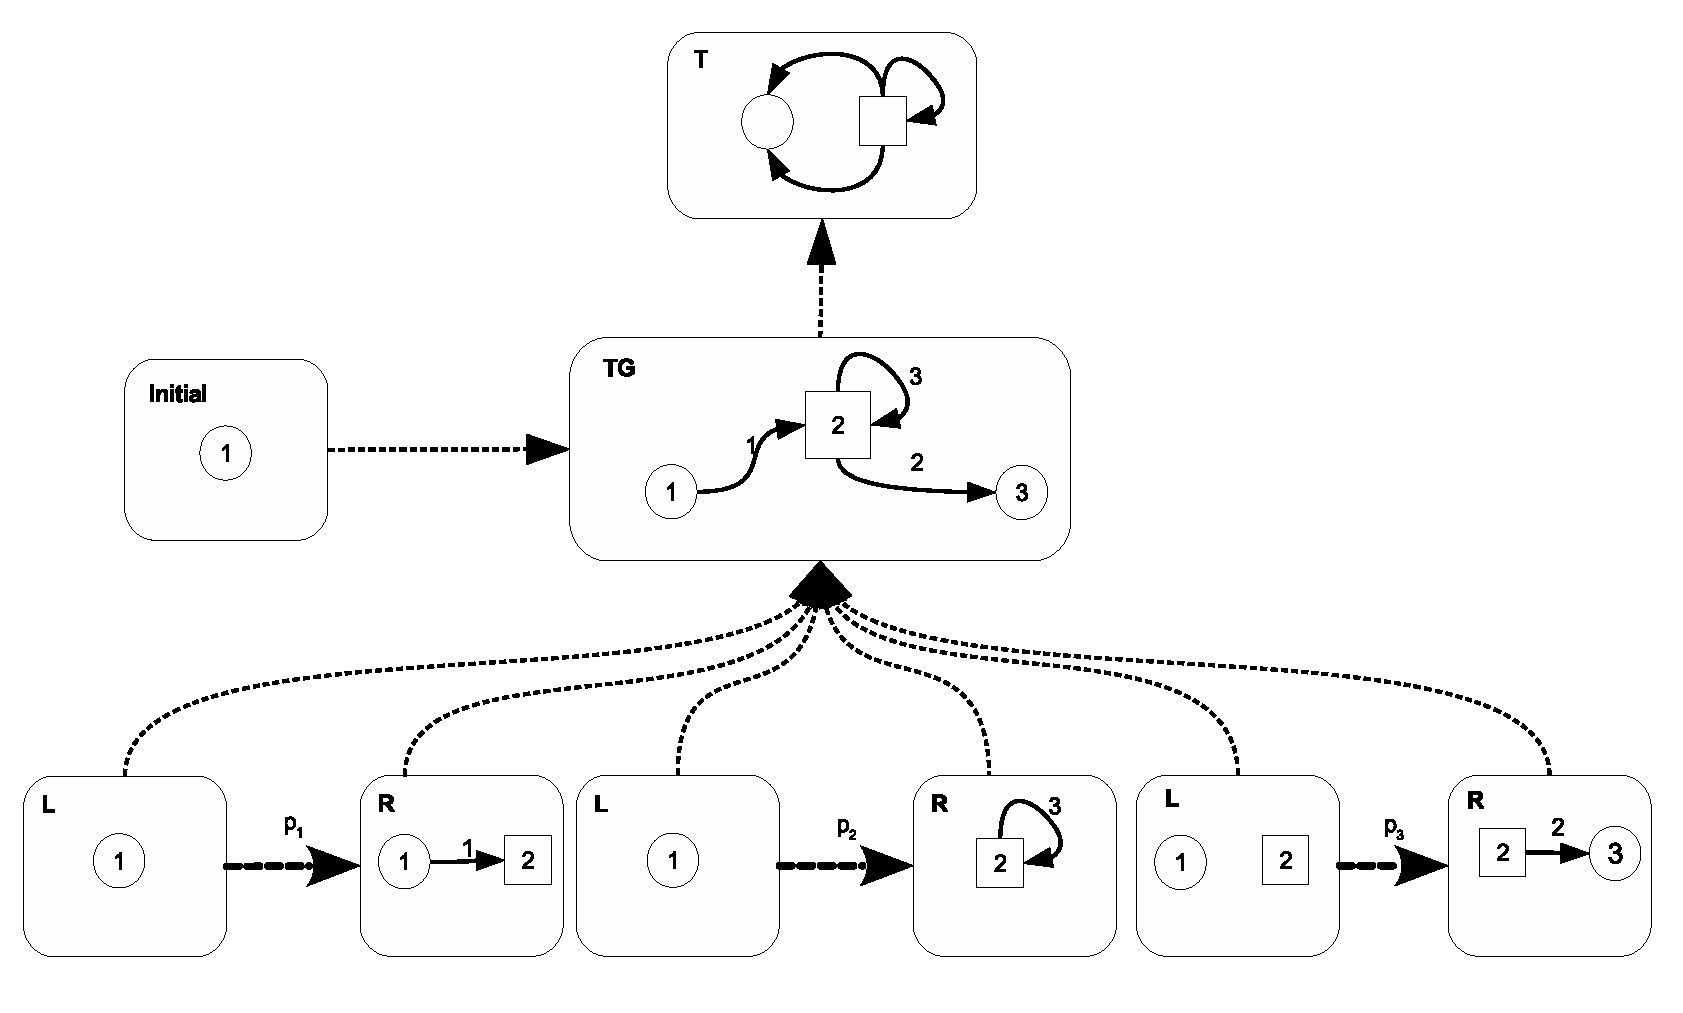
\includegraphics[scale=0.5]{images/process/core_graph/counter_example}}}
    \caption{A grammar with a double-type graph that is not a core graph.}\label{fig:process:core-graph:counter-example}
  \end{subfigure}
  \begin{subfigure}[t]{.5\textwidth}
    \centerline{\fbox{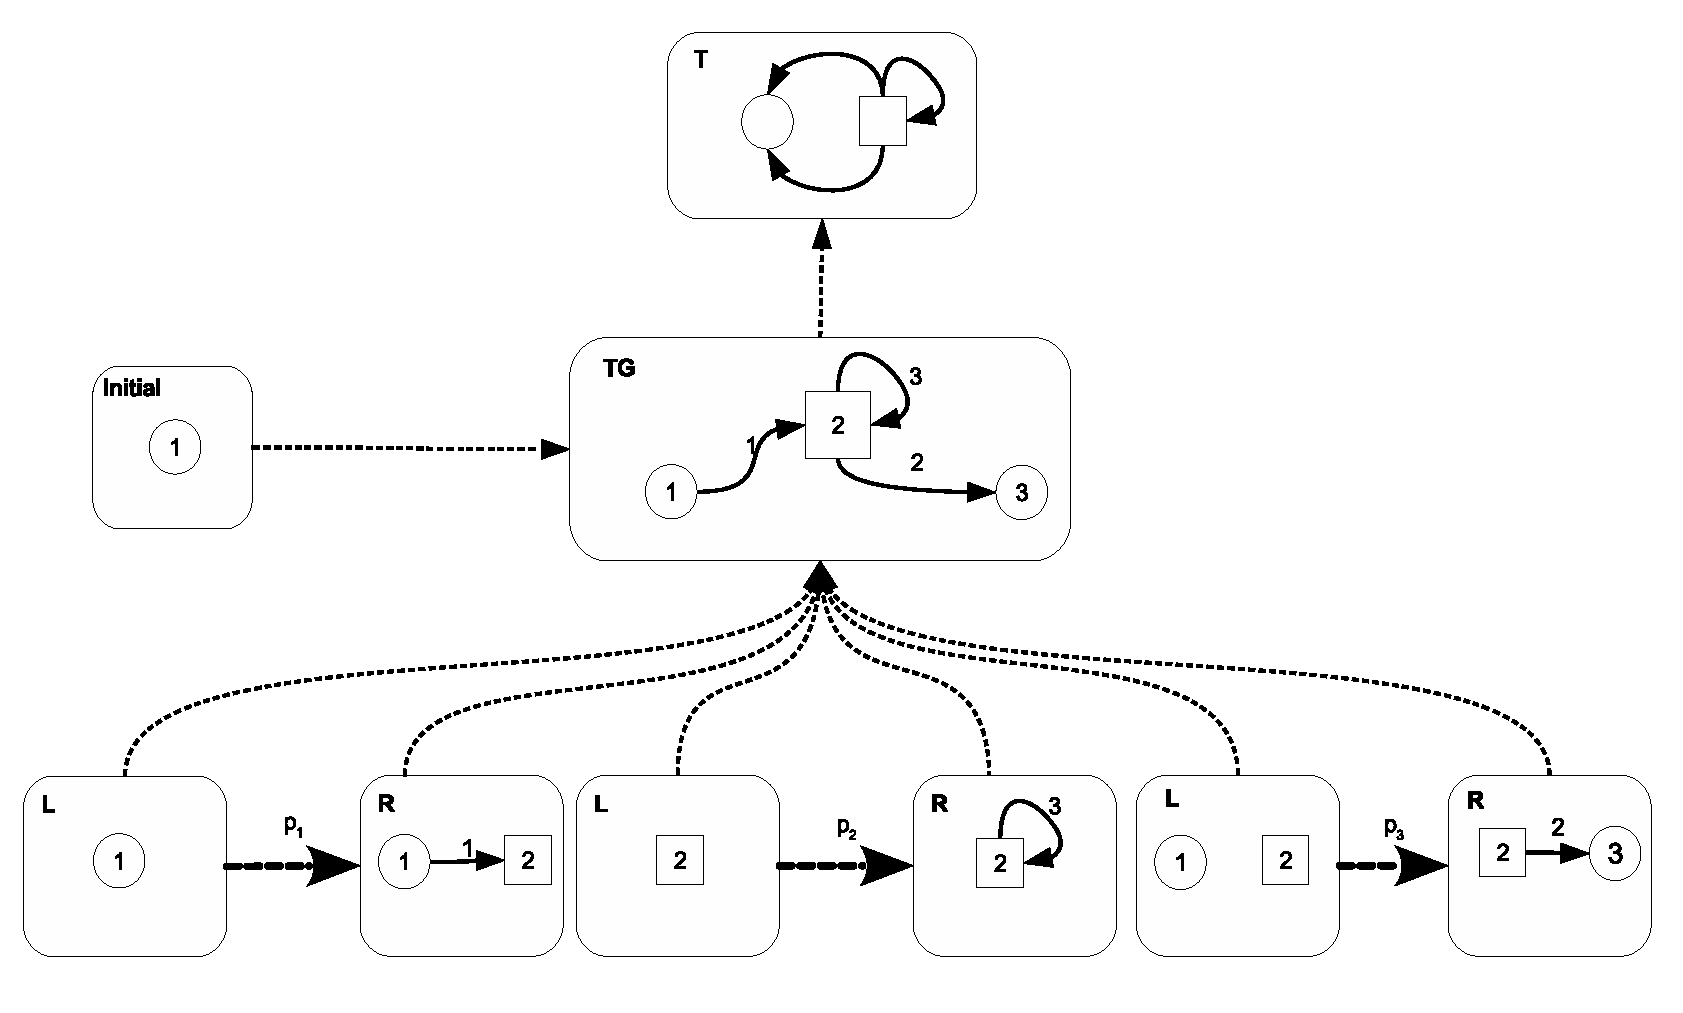
\includegraphics[scale=0.5]{images/process/core_graph/example}}}
    \caption{A grammar with a double-type graph that is also a core graph.}\label{fig:process:core-graph:example}
  \end{subfigure}

  \caption{Doubly-typed graph grammars}\label{fig:process:doubly-typed-grammars}
\end{figure}

\end{example}

\begin{definition}[Strongly Safe (Doubly-Typed) Graph Grammars] Given \doublyTypedGraphGrammarCore{} a doubly-typed graph grammar, $GG$ is said to be \emph{strongly safe} if its double-type graph is also a core graph.

  Each rule in a strongly safe graph grammar is also called an \emph{action}. We say that an action $a$ creates an element $e$ iff $e \in R(a) - K(a)$. Similarly, $a$ deletes $e$ iff \mbox{$e \in L(a) - K(a)$}.
\end{definition}

\begin{remark}[Strongly Safe Grammars] Throughout this work, we will use only strongly safe grammars whose set $P$ of actions is finite and each action in $P$ is distinct from the others.
\end{remark}

\begin{example}[Strongly Safe Graph Grammar] Figure~\ref{fig:process:core-graph:example} also depicts a strongly safe graph grammar as the double-type graph of the grammar is, in fact, a core graph.
\end{example}

\section{Relations within Strongly Safe Graph Grammars without NACs}

Given a strongly safe graph grammar, its core graph contains all elements used (created, read or deleted) during one possible execution of the grammar. Moreover, as each element has a unique origin within it, the core graph can be considered to contain the entire ``execution history'' of its underlying grammar.

We are here interested in some of the properties that can be found by looking at this history. Particularly, which kind of relations exist among actions and elements, whether it is possible to find sequences in which all actions are applied and which graphs can be considered valid (reachable) by this grammar.

In~\cite{Ribeiro1996}, causal, conflict and occurrence relations for strongly safe graph grammars were defined. There, the graph transformation approach used was the \emph{Single Pushout} (SPO) without NACs.

\cite{Corradini1996} also defined a different notion of causal relation, equivalent to the occurrence relation in the previous mentioned work, with respect to the DPO approach without NACs.

Both authors use these relations to find out whether all the actions of a strongly safe graph grammar are applicable and prove some properties about it\tinytodo{which properties?}. However, this relations alone are not sufficient for our purpose when the actions may have NACs, which are nowadays essential for modelling complex systems~\cite{Corradini2014}\tinytodo{Redo this paragraph, explain better our needs}.

Here we recall these definitions, which correspond to the \emph{existential relation} and the \emph{unconditional causal dependency and conflict relations} defined in the following, and extend them to create an equivalent notion of \emph{conditional relations} that work for grammars in the DPO approach with NACs.

\begin{notation}[Restriction to Image] Given an arbitrary morphism $f : A \rightarrow X$, we will denote as $f' : A \rightarrow X_{|A}$ the morphism derived from $f$ where $X_{|A}$ is the image of $f$. As a consequence, $X_{|A}$ contains all and only the elements of $X$ that are somehow mapped from $A$ to $X$, preserving the original mapping.

  For two arbitrary morphisms $f : A \rightarrow X$ and $g : B \rightarrow X$, we will denote as $f' : A \rightarrow X_{|AB}$ and $g' : B \rightarrow X_{|AB}$ the morphisms derived from $f$ and $g$ where $X_{|AB}$ is the jointly image of both $f$ and $g$. As a result, $X_{|AB}$ contains all and only the elements of $X$ that are mapped from $A$ or $B$ to $X$, preserving the original mappings.
\end{notation}

\begin{remark}[Different Graph Transformation Interpretation] When dealing with actions, we will use a slightly different interpretation for the graph transformations:
  
First, actions are always applied over the core graph: the match of an action is equal to its pre-condition $pre_a : L \rightarrow C^T$, as well as the comatch is equal to its post-condition $post_a : R \rightarrow C^T$. 
  
  Second, elements in $pre_a - k_a$ and $post_a - k_a$ are not ``really'' deleted nor created on the core graph (since they must always be present in the core graph as it maintains the history of execution), but rather annotated as deleted or created w.r.t. to an action. Nonetheless, their creation (resp. deletion) would be performed in an execution of the underlying simply-typed grammar. Here, for the sake of simplicity, we overload these terms and continue to refer to this elements as created/deleted.

  Third, given an action $a$ with NACs and its underlying graph transformation, we restrict the search of the injective morphism $q : N \rightarrow C^T$ to the image of the match $q : N \rightarrow C^T_{L_a}$ (comatch $q : N \rightarrow C^T_{R_a}$) rather than the entire core graph. Similarly, when searching for conflicts or dependencies within two actions $a_1, a_2$ with NACs, the test of NAC satisfiability performed on the overlapping between the actions is restricted to the jointly image of the respective morphisms onto the core graph.

  The ``restricted to the image'' search is meant to avoid the triggering of NACs by elements that are present in the core graph, therefore present in the match/comatch, but that do not exist when looking only at the actions interacting at the moment. \tinytodo{It also avoids the dangling condition in the core graph out of the scope of the actions, find the proper place to explain it.} This restriction together with the use of incremental NACs allow us to locally compute the conflicts and dependencies for each pair of actions, without having to be concerned about global effects of other actions coming into play.
\end{remark}

\begin{definition}[Existential Relation] \tinytodo{I need a better name for this relation}This is the \emph{causal relation} defined in \cite{Corradini1996} for the DPO approach without NACs. Given  \doublyTypedGraphGrammarCore{} a strongly safe graph grammar. Let actions \mbox{$a_1, a_2 \in P, a_1 \ne a_2$} and element \mbox{$e_1 \in N(C^T) \cup E(C^T)$}, then:

  \begin{enumerate}
    \item If $a_1$ deletes $e_1$, then $e_1 <_e a_1$.
    \item If $a_1$ creates $e_1$, then $a_1 <_e e_1$.
    \item If $a_1$ creates $e_1$ and $a_2$ preserves $e_1$, then $a_1 <_e a_2$.
    \item If $a_1$ preserves $e_1$ and $a_2$ deletes $e_1$, then $a_1 <_e a_2$. 
    \item The \emph{existential relation} $\leq_e$ of $P \cup N(C^T) \cup E(C^T)$ is the reflexive and transitive closure of $<_e$.
  \end{enumerate}
\end{definition}

This relation represents restrictions over creation, use (preservation) and deletion of elements by actions that must be respected for the actions to be applicable. In other words, an action $a$ must occur after all the actions that create the elements which it depends on. Analogously, $a$ must occur before all actions that delete those same elements.

In \cite{Corradini1996} it is shown that if this relation is a \emph{partial order}, then there exists at least one total order in respect to it in which all productions of the underlying grammar are applicable. However, this condition is not sufficient in grammars whose rules may be equipped with NACs, as shown in example~\ref{ex:process:existential-relation-fail}.

\begin{example}[Existencial Relation in Grammars without NACs]\label{ex:process:existential-relation} Given the strongly safe grammar corresponding to the core and initial graphs in Figure~\ref{fig:process:existential-relation:core-graph} and the set of rules in Figure~\ref{fig:process:existential-relation:example}, we have that:

\begin{itemize}
  \item $a_1 <_e \triangle_2$
  \item $a_2 <_e \Square_1$ and $a_2 <_e$ $\curvearrowleft_1$
  \item $a_3 <_e$ $\curvearrowleft_2$
  \item $a_2 <_e a_1$ by creation/preservation of $\Square_1$
\end{itemize}

  The existential relation for this grammar is (without the pairs due to reflexivity): \tinytodo{Mount transitive and reflexive closure}.

  Therefore, we have that all actions in this grammar can be applied as long as $a_2$ is applied before $a_1$ ($a_2$ crates the element $\Square_1$ which is necessary for $a_1$ to be applied). In particular, the following configurations are valid and lead to the same result: $[a_2,a_1,a_3],[a_2,a_3,a_1],[a_3,a_2,a_1]$.

\begin{figure}[!ht]
  \centering
  \begin{subfigure}[t]{.5\textwidth}
    \centerline{\fbox{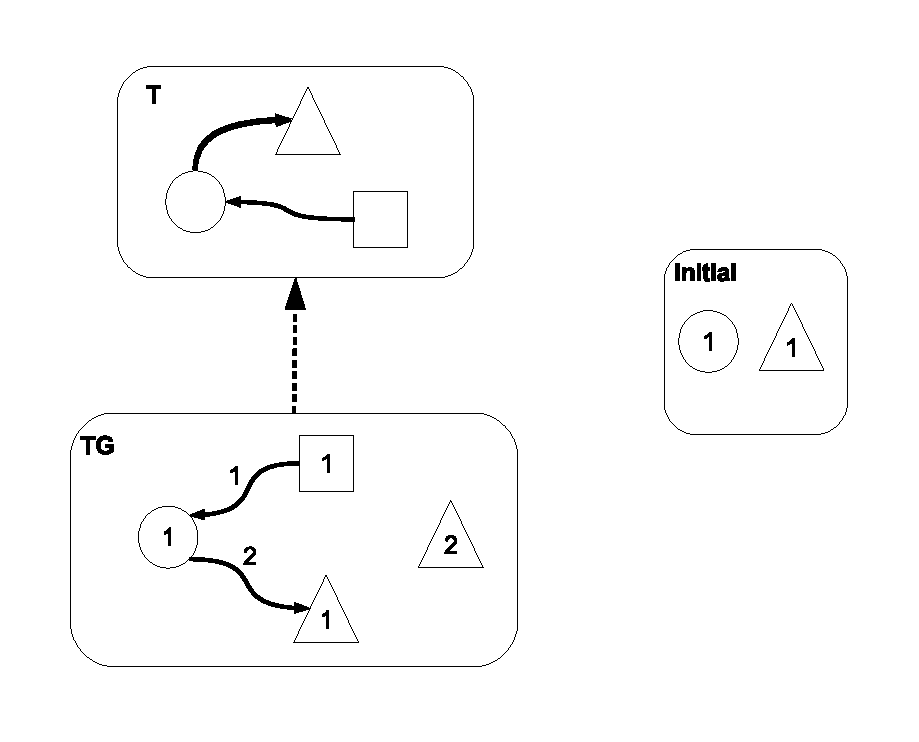
\includegraphics[scale=0.6]{images/process/existential-relation/core-graph}}}
    \caption{Core and initial graphs}\label{fig:process:existential-relation:core-graph}
  \end{subfigure}
  \begin{subfigure}[t]{.5\textwidth}
    \centerline{\fbox{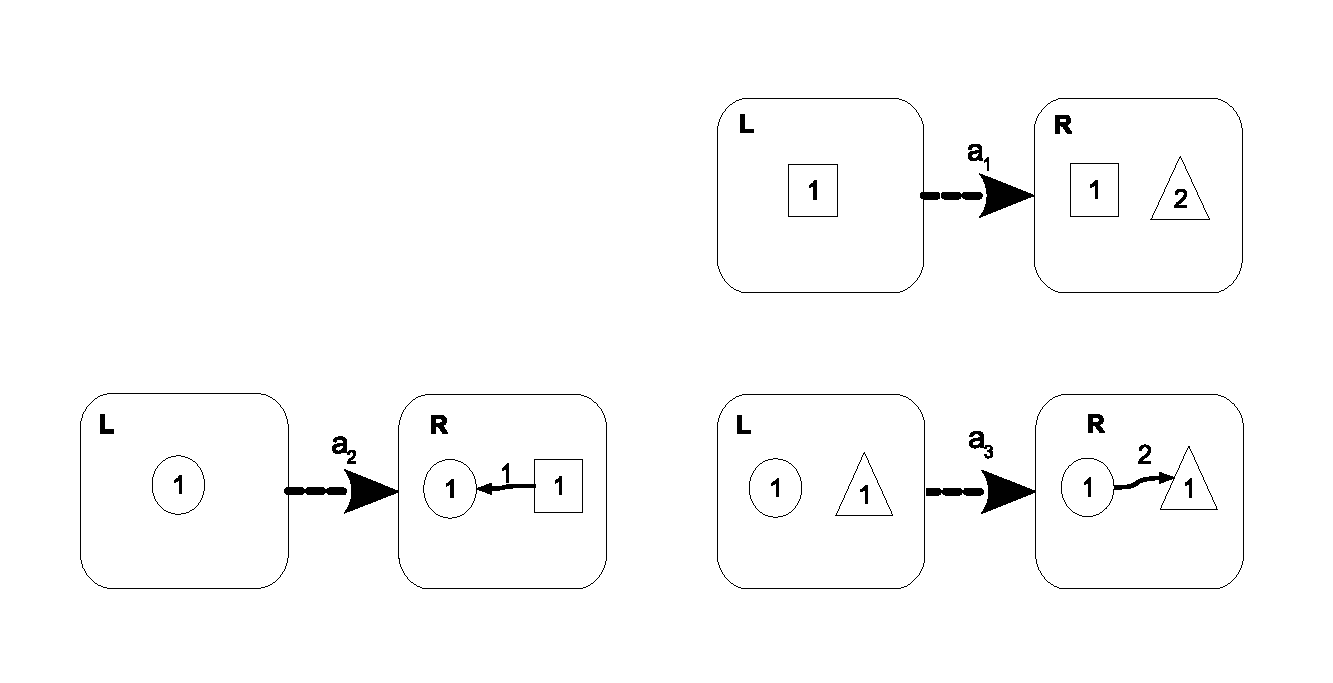
\includegraphics[scale=0.6]{images/process/existential-relation/example}}}
    \caption{A strongly safe grammar without NACs}\label{fig:process:existential-relation:example}
  \end{subfigure}
  \begin{subfigure}[t]{.5\textwidth}
    \centerline{\fbox{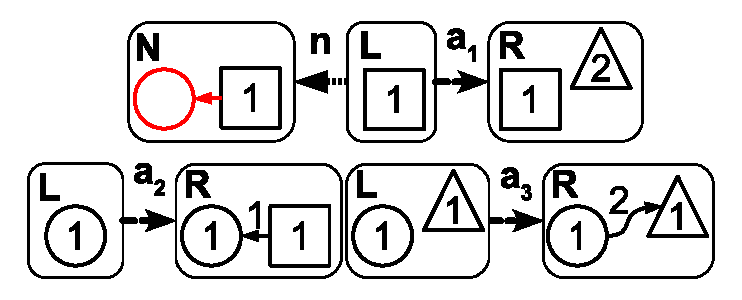
\includegraphics[scale=0.6]{images/process/existential-relation/example-nacs}}}
    \caption{A strongly safe grammar with NACs}\label{fig:process:existential-relation:example-nacs}
  \end{subfigure}
  \stepcounter{doubly-typed-grammar-counter}
  \caption{Strongly safe grammar GG\arabic{doubly-typed-grammar-counter}}\label{fig:process:existential-relation}
\end{figure}
\end{example}

The same definition can be attempted in a strongly safe grammar where actions are equipped with Nacs. However, as shown in the next example, it lacks the same properties as the relation in the context without NACs.

\begin{example}[Existential Relation in Grammars with NACs]\label{ex:process:existential-relation-fail}Consider the strongly safe grammar corresponding to the core and initial graphs in Figure~\ref{fig:process:existential-relation:core-graph} and the set of rules in Figure~\ref{fig:process:existential-relation:example-nacs}. 
  
  We have the same the same existential relation as the one presented in Example~\ref{ex:process:existential-relation}, since the structure of the actions are the same in both examples, except for the NAC in the action $a_1$ on Figure~\ref{fig:process:existential-relation:example-nacs}.

  Following this example, we still have that $a_2$ must be applied first in order for $a_1$ to be applied. However, besides creating the $\Square_1$ needed for $a_1$, $a_2$ also creates a $\curvearrowleft_1$ from $\Square_1$ to $\Circle_1$ which is a pattern forbidden by NAC of $a_1$. Therefore, we have that $a_2$ also causes a \emph{produce-forbid} conflict with $a_1$.

  Moreover, the only other action $a_3$ does not delete any element that could help undoing the forbidden pattern. Thus, there is no possible way of applying all actions of this grammar, even though the existential relation is a partial order.

\end{example}

The next \emph{unconditional relations} are equivalent to the \emph{causal dependency} and \emph{weak conflict} relations presented at~\cite{Ribeiro1996}, but for the DPO approach, rather than the SPO one. Furthermore, \emph{conditional relations} will be later defined for conflicts and dependencies with NACs.

Regarding both unconditional and conditional dependency relations, their definitions are based on the following intuition:

\begin{intuition} An action $a_1$ is a direct cause of an action $a_2$ if either $a_1$ creates some element that is needed by $a_2$ (unconditional causal dependency) or $a_1$ deletes an element that is both forbidden by a NAC of $a_2$ and existent before the application of $a_2$ (conditional causal dependency). In both cases, we have that $a_2$ can only happen after $a_1$ has been applied.\tinytodo{Explain that we do not use the notion of irreversible dependency, as we are interested only in the ordered
  execution of the actions?} 
\end{intuition}

\begin{figure}[!ht]
  \centering
  \begin{subfigure}[t]{.5\textwidth}
    \centerline{\fbox{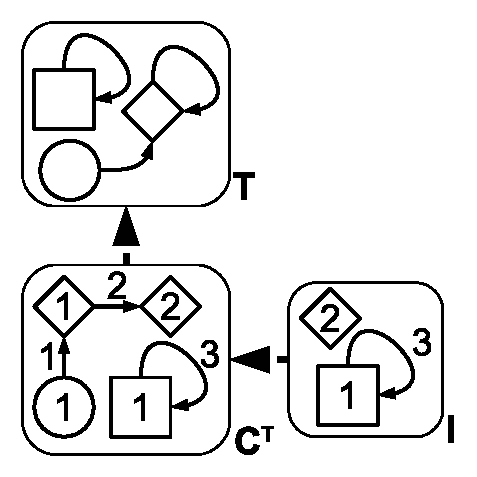
\includegraphics[scale=0.5]{images/process/unconditional-relation/core-graph}}}
    \caption{Core and initial graphs}\label{fig:process:unconditional-relation:core-graph}
  \end{subfigure}

  \begin{subfigure}[t]{.5\textwidth}
    \centerline{\fbox{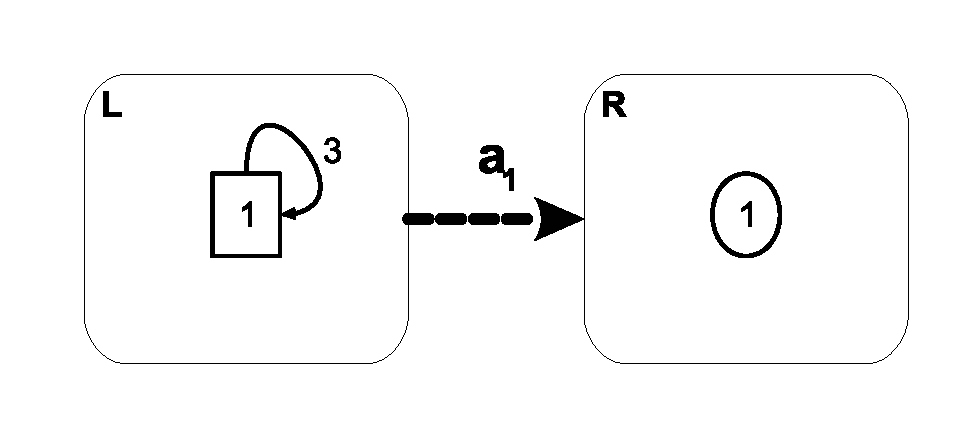
\includegraphics[scale=0.45]{images/process/unconditional-relation/a1}}}
    \caption{Action $a_1$}\label{fig:process:unconditional-relation:a1}
  \end{subfigure}%
  \begin{subfigure}[t]{.5\textwidth}
    \centerline{\fbox{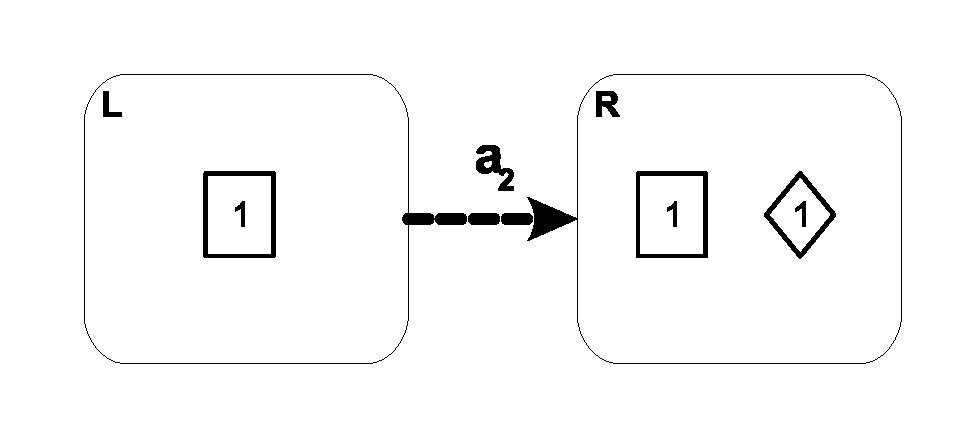
\includegraphics[scale=0.45]{images/process/unconditional-relation/a2}}}
    \caption{Action $a_2$}\label{fig:process:unconditional-relation:a2}
  \end{subfigure}

  \begin{subfigure}[t]{.5\textwidth}
    \centerline{\fbox{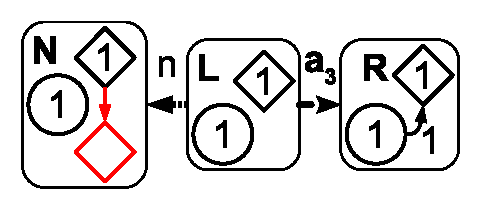
\includegraphics[scale=0.45]{images/process/unconditional-relation/a3}}}
    \caption{Action $a_3$}\label{fig:process:unconditional-relation:a3}
  \end{subfigure}%
  \begin{subfigure}[t]{.5\textwidth}
    \centerline{\fbox{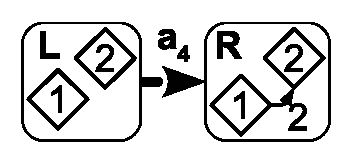
\includegraphics[scale=0.45]{images/process/unconditional-relation/a4}}}
    \caption{Action $a_4$}\label{fig:process:unconditional-relation:a4}
  \end{subfigure}
  \stepcounter{doubly-typed-grammar-counter}
  \caption{Strongly safe grammar GG\arabic{doubly-typed-grammar-counter}}\label{fig:process:unconditional-relation}
\end{figure}

\begin{definition}[Unconditional Causal Dependency Relation\footnote{Also called Produce-Use Relation.}]\label{def:unconditional-causal-dependency} Given \doublyTypedGraphGrammarCore{} a strongly safe graph grammar. Let $a_1, a_2 \in P$, $a_1 \ne a_2$, \mbox{$e_1, e_2 \in $ \coreGraph{}} and $e_1 \ne e_2$. Then: 

  \begin{enumerate}
    \item The action $a_2$ is \emph{directly causally dependent} on $a_1$, written $a_1 <_{pu} a_2$, iff \mbox{$\not\exists h_{21} : L_2 \rightarrow D_1$ s.t. \mbox{$d_1 \circ h_{21} = pre_2$}}, where the two squares are pushouts and $C^T_{|R_1L_2}$ ($C^T$ restricted to the jointly-image of $post_1$ and $pre_2$) satisfies the NACs for $a_2$ and $a_1^{-1}$.

\diagram{
   & & N_1^{-1} & & N_2 & & \\
      L_1 & K_1\ar[d]\ar[l]\ar[r] & R_1\ar[u]\ar[dr]_{post_1} & & L_2\ar[u]\ar@{.>}@/_1.1pc/[dlll]|{|}_<<<<{h_{21}}\ar[dl]^{pre_2} & K_2\ar[l]\ar[r]\ar[d] & R_2\\
       & D_1\ar@{^{(}->}[rr]_{d_1} & & C^T_{|R_1L_2} & & D_2\ar@{_{(}->}[ll]^{e_2} &}

   \item The \emph{causal dependency relation between actions} $\leq_{pu}$ of $P$ is the reflexive and transitive closure of the direct causal dependency.
   \item The element $e_2$ is \emph{directly causally dependent} on $e_1$, written $e_1 <_{pu} e_2$, iff there is an action $a_1 \in P$ such that $a_1$ deletes $e_1$ and creates $e_2$.
   \item The \emph{causal dependency relation between elements} $\leq_{pu}$ of $N(C^T) \cup E(C^T)$ is the reflexive and transitive closure of the direct causal dependency.
   \item The \emph{unconditional causal dependency relation} of a strongly safe grammar is defined as the transitive and reflexive closure of the union of both relations $\leq_{pu}$ for $P$ and $N(C^T) \cup E(C^T)$.
  \end{enumerate}
\end{definition}

\begin{example}[Unconditional Dependency Example]Figure~\ref{fig:process:unconditional-relation:dependency} \tinytodo{review the names of the graphs} shows a produce-use between the actions $a_2$ and $a_4$ of the strongly safe grammar depicted in Figure~\ref{fig:process:unconditional-relation}.

  This conflict occurs due to the fact that, besides both actions have valid graph transformations (they satisfy the rewriting conditions for the overlapping on $C^T$ restricted do the image of $post_2$ and $pre_4$ and none of them has any NACs), it is not possible to find a morphism from $L_4$ to $D_2$ satisfying the conditions on Definition~\ref{def:unconditional-causal-dependency}.

\begin{figure}[!ht]
  \centering
  \fbox{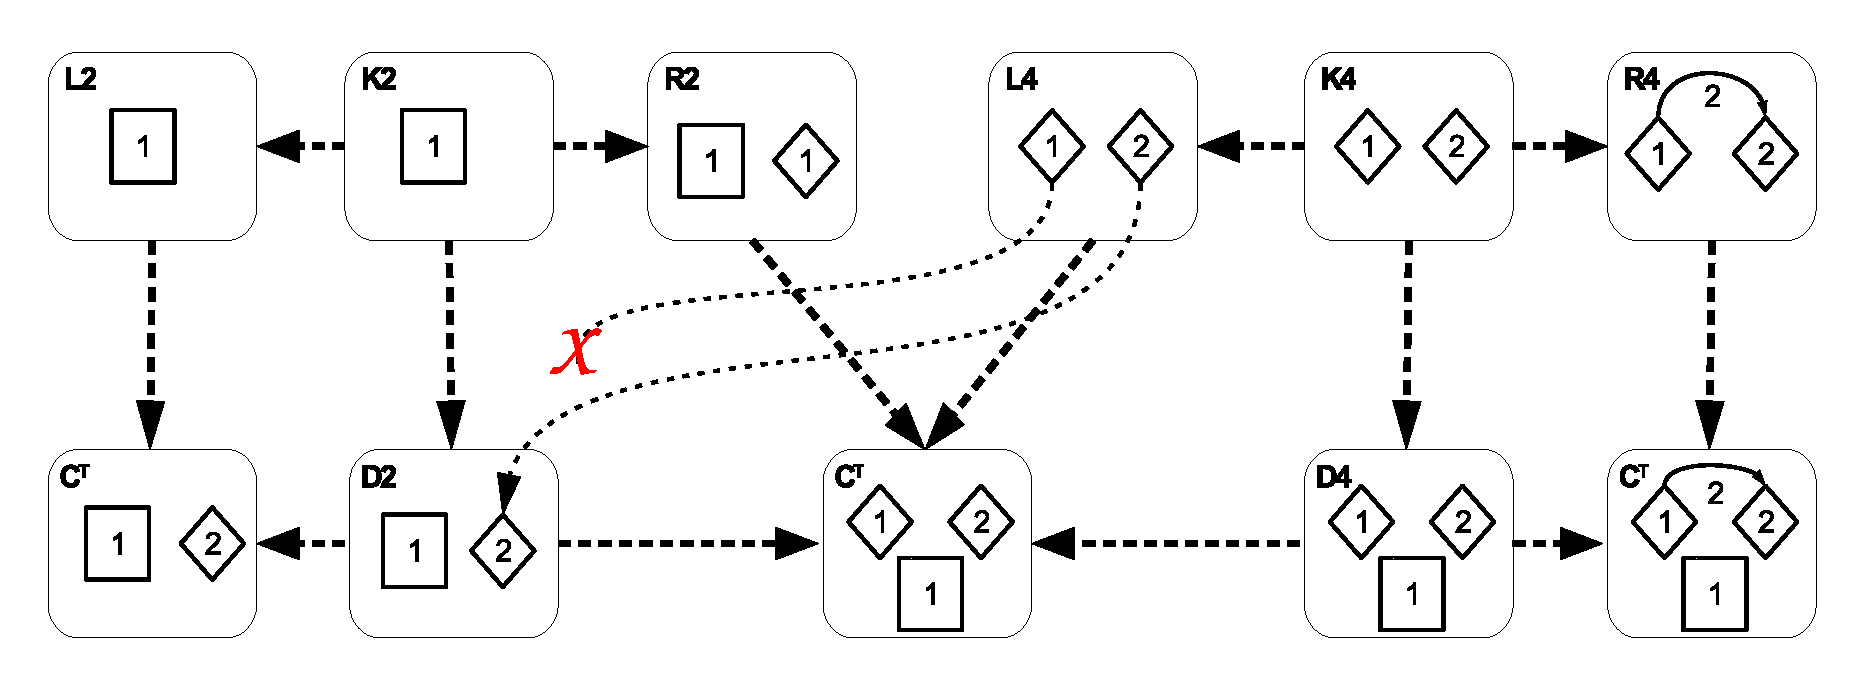
\includegraphics[scale=0.48]{images/process/unconditional-relation/dependency}}
  \caption{Unconditional causal dependency situation}\label{fig:process:unconditional-relation:dependency}
\end{figure}
\end{example}

Regarding both unconditional and conditional weak conflict relations, their definitions are based on the following intuition:

  \begin{intuition} An action $a_1$ is in \emph{weak} conflict with an action $a_2$ if either $a_1$ deletes something that is needed by $a_2$ to be applied (unconditional weak conflict) or creates something that is both forbidden by a NAC of $a_2$ and not deleted before the application of $a_2$ (conditional weak conflict). In both cases, we have that $a_2$ can not be applied once $a_1$ has been applied, in other words, $a_2$ can only be applied before $a_1$.
\end{intuition}

\begin{definition}[Unconditional Weak Conflict Relation\footnote{Also called Delete-Use Relation.}]\label{def:unconditional-conflict} Given \doublyTypedGraphGrammarCore{} a strongly safe graph grammar. Let $a_1, a_2 \in P$, $a_1 \ne a_2$, \mbox{$e_1, e_2 \in $ \coreGraph{}} and $e_1 \ne e_2$. Then: 

  \begin{enumerate}
    \item The action $a_1$ is in \emph{direct weak conflict} with $a_2$, written $a_2 <_{du} a_1$, iff \mbox{$\not\exists h_{21} : L_2 \rightarrow D_1$} s.t. \mbox{$d_1 \circ h_{21} = pre_2$}.

      \diagram{
          & & N_1 & & N_2 & & \\
        R_1 & K_1\ar[l]\ar[r]\ar[d] & L_1\ar[u]\ar[dr]_{pre_1} & & L_2\ar[u]\ar[dl]^{pre_2}\ar@{.>}@/_1.1pc/[dlll]|{|}_<<<<{h^{21}} & K_2\ar[l]\ar[r]\ar[d] & R_2\\
       & D_1\ar[rr]_{d_1} & & C^T_{|L_1L_2} & & D_2\ar[ll] &}
   \item The \emph{weak conflict relation between actions} $\leq_{du}$ of $P$ is the reflexive and transitive closure of the direct weak conflict.
   \item The element $e_2$ is \emph{in direct weak conflict} with $e_1$, written $e_2 <_{du} e_1$, iff there are actions $a_1$ and $a_2$ that respectively create $e_1$ and $e_2$ and $a_2 \leq_{du} a_1$.
   \item The \emph{weak conflict relation between elements} $\leq_{du}$ of $N(C^T) \cup E(C^T)$ is the reflexive and transitive closure of the direct weak conflict.
   \item The \emph{weak conflict relation} of a strongly safe grammar is defined by transitive and reflexive closure of the unions of relations $\leq_{du}$ for $P$ and $N(C^T) \cup E(C^T)$.

  \end{enumerate}
\end{definition}

\begin{example}[Unconditional Weak Conflict Example] Figure~\ref{fig:process:unconditional-relation:conflict} shows a delete-use between the actions $a_1$ and $a_2$ of the strongly safe grammar depicted in Figure~\ref{fig:process:unconditional-relation}.

  Again, both actions have valid graph transformations, now for the overlapping of $pre_1$ and $pre_2$ on $C^T$, but it is not possible to find a morphism from $L_2$ to $D_1$ satisfying the conditions on Definition~\ref{def:unconditional-conflict}.
\begin{figure}[!ht]
  \centering
  \fbox{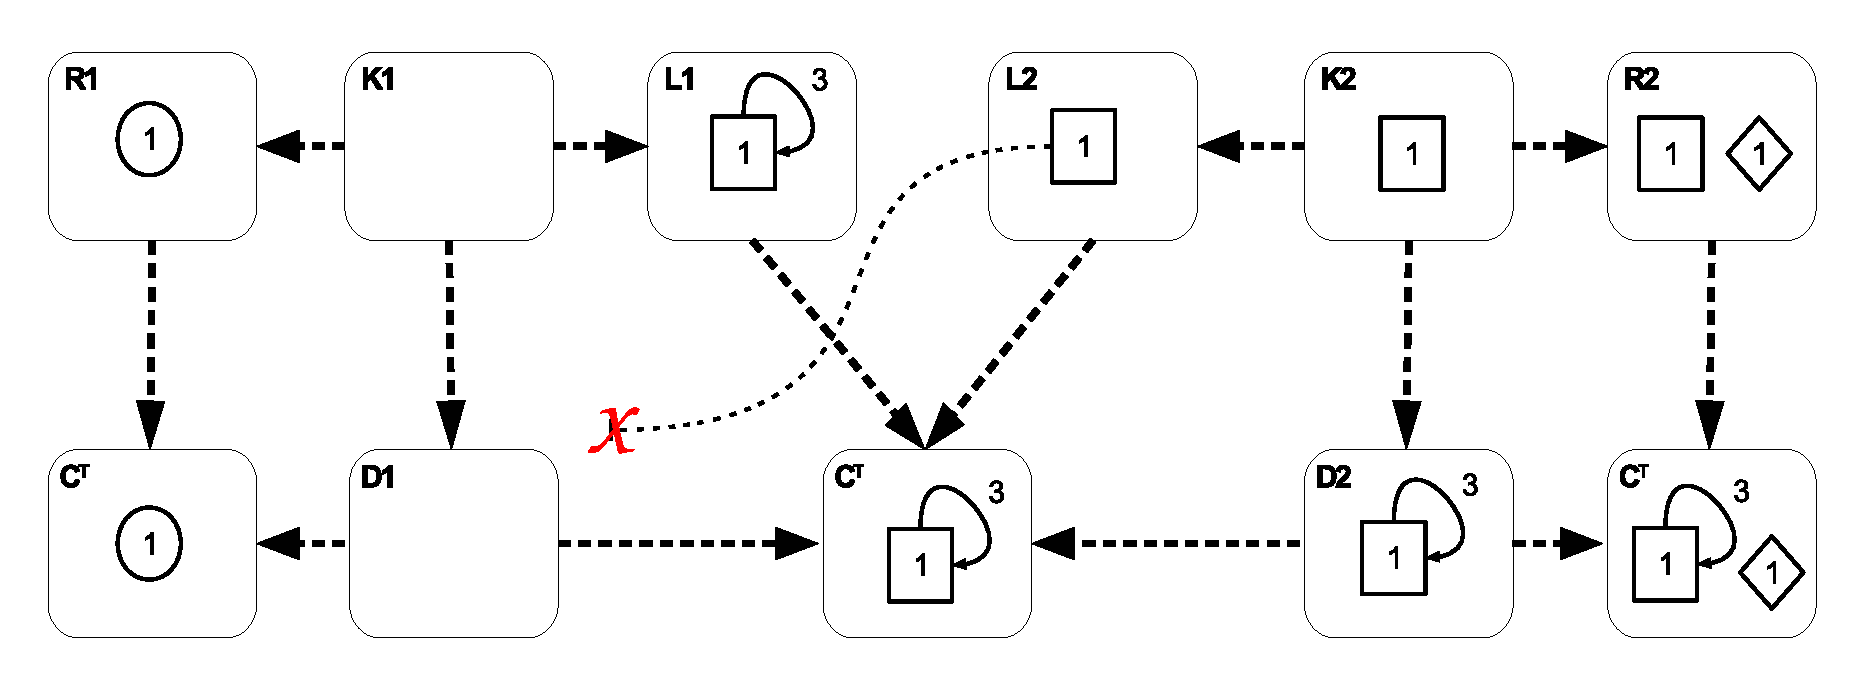
\includegraphics[scale=0.48]{images/process/unconditional-relation/conflict}}
  \caption{Unconditional weak conflict situation}\label{fig:process:unconditional-relation:conflict}
\end{figure}
\end{example}

\begin{definition}[Unconditional Occurrence Relation] Given \doublyTypedGraphGrammarCore{} a strongly safe graph grammar, let $\leq_{pu}$ and $\leq_{du}$ be the unconditional dependency and unconditional weak conflict relations of this grammar for $P \cup N(C^T) \cup E(C^T)$. Then the \emph{unconditional occurrence relation} of GG is the reflexive and transitive closure of \mbox{$\leq_{pu} \cup \leq_{du}$}.
\end{definition}

Similarly to the existential relation,~\cite{Ribeiro1996} proved that if this relation is a partial order, then it is possible to apply all actions of its underlying grammar in any total order that respects the partial order. Again, this condition is not sufficient if the rules may be equipped with NACs\tinytodo{is it necessary to draw another example?}, as it was also shown to be equivalent to the existential relation.

\begin{example}[Unconditional Relations] \tinytodo{Create at least one more rule to show the transitive closure working} For the strongly safe grammar depicted on Figure~\ref{fig:process:unconditional-relation} we have the following relations: 

\begin{itemize}
  \item produce-use dependencies: $a_1 <_{pu} a_3$, $a_2 <_{pu} a_3$, $a_2 <_{pu} a_4$. Therefore, the unconditional dependency relation for the actions is $a_1 \leq_{pu} a_3$, $a_2 \leq_{pu} a_3$, $a_2 \leq_{pu} a_4$. 
  \item delete-use conflicts\tinytodo{define unconditional occurrence relation}: $a_2 <_{du} a_1$. Therefore, the unconditional weak conflict relation for the actions is $a_2 \leq_{du} a_1$.
  \item unconditional occurrence relation: $a_1 \leq a_3$, $a_2 \leq a_3$, $a_2 \leq a_4, a_2 \leq a_1$.
\end{itemize}

  In order to know if all the actions of a strongly safe grammar without NACs can be applied, it would be sufficient to check whether the unconditional occurrence relation is a partial order.

  In particular, if we do not consider the NACs for the grammar in Figure~\ref{fig:process:unconditional-relation}, any total order of action compatible with the partial order given by the unconditional occurrence relation would be a valid sequentialization of this grammar. As an example, $[a_2, a_1, a_3, a_4]$ and $[a_2, a_4, a_1, a_3]$ are valid serializations (without NACS) for this grammar. 
  
  However, not all previous serializations are valid when NACs come into play. Specifically, the sequence $[a_2, a_4, a_1, a_3]$ is not valid, because if $a_4$ is applied before $a_3$ it creates $\curvearrowleft_2$, triggering the NAC of $a_3$ which can no longer be applied.

\end{example}

\begin{remark}[Existential and Unconditional Occurrence Relations] Since the \emph{existential} and \emph{unconditional occurrence relations} where shown to be equivalent by~\cite{Ribeiro1996}, we will only one of them, the \emph{existential relation}, as the standard relation without without NACs from now on, as it was originally defined for DPO grammars.

  However, we were heavily inspired by the structure of the \emph{unconditional causal dependency} and \emph{unconditional weak conflict relations} to define the relations with NACs.
\end{remark}

\section{Relations within Strongly Safe Graph Grammars with NACs}

The previous relations extracted from strongly safe grammars have the property of being always concrete, in the sense that if an action is dependent on (conflicting with) another one, it happens because the one of them creates (resp. deletes) at least one of the concrete elements necessary for the other to be applied (resp. prevented of being applied).

Moreover, the existential relation must always be respected whenever we try to find a total order in which all the actions of a strongly safe grammar are applicable. However, for grammars equipped with NACs it is necessary to include the conflicts and dependencies created by NACs in this relation.

The problem here is that we can not just add the conflicts and dependencies caused by NACs directly into the existential relation (as was the case for their unconditional counterparts in the unconditional occurrence relation) because they are not always concrete. This means that depending on the total order of application chosen among the possibilities given by the existential relation, a conflict or dependency may or may not happen.

In fact, according to the possible application orders, such dependencies and conflicts may be classified as \emph{concrete}, they will happen no matter the chosen order; \emph{non existent}, they will never happen no matter the order; or \emph{abstract}, they may occur in only in some total orders.

\begin{example}[Interaction between existential relation and NACs]
Let $a_1, a_2, a_3$ be three actions of the same strongly safe grammar. Suppose that $a_1$ creates elements used by $a_2$ and $a_2$ creates elements used by $a_3$, therefore by the existential relation we know that $a_1 \leq_e a_2 \leq_e a_3$.

  Now suppose that when $a_2$ is applied, it creates an element that would be forbidden by a NAC of $a_1$ and also that $a_3$ deletes this element. Following the classical notions of dependency and conflict with NACs, as shown in definitions~\ref{def:classic-dependency} and~\ref{def:classic-conflict}, $a_2$ would cause a produce-forbid conflict on $a_1$ $(a_1 <_{pf} a_2)$, while $a_1$ would be dependent by delete-forbid on $a_3$ $(a_3 <_{df} a_1)$.
  
  Adding these produce-forbid and delete-forbid directly to the existential relation we would have the situation depicted in Figure~\ref{fig:process:order:occurrence-relation-fail}. It is easy to see that the resulting relation is not a partial order, therefore there can be no total ordering for this set of actions.
\begin{figure}[!ht]
  \centering
  \fbox{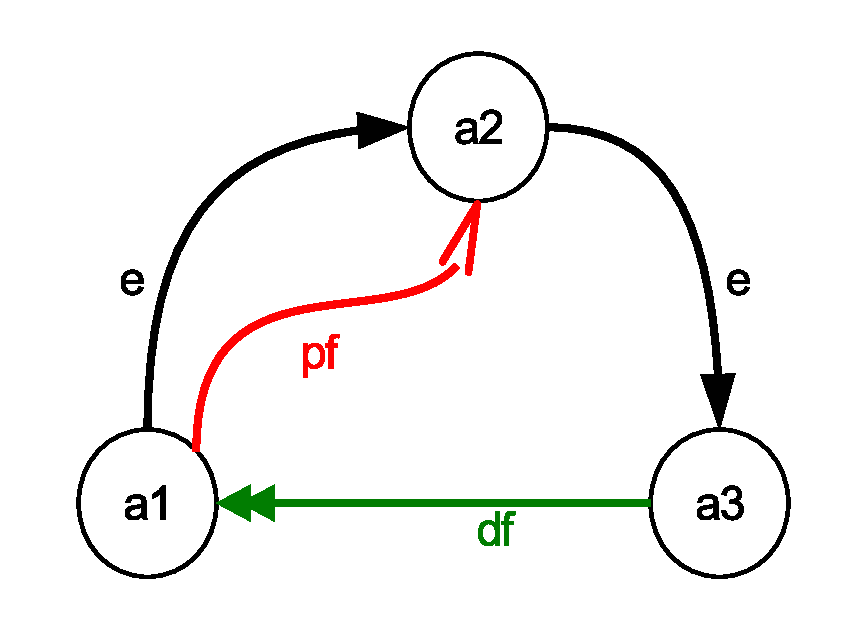
\includegraphics[scale=0.5]{images/process/order/occurrence-relation-fail}}
  \caption{Graph of relations}\label{fig:process:order:occurrence-relation-fail}
\end{figure}

However, looking at the existential relation, we can affirm that this configuration ensures that neither the conflict nor the dependency exist in any concrete execution of this grammar. 

  For the conflict, this happens because $a_2$ can only happen after $a_1$, thus the element forbidden by the NAC of $a_1$ can only exist after $a_1$ itself was already applied. Likewise, the dependency that is identified because $a_3$ deletes the element that would be forbidden by the NAC of $a_1$ does not exist either.\tinytodo{Draw the examples for non existent (last paragraph), concrete and potential
dependencies/conflicts}. 
\end{example}

We already know that at least the existential relation must be a partial order in order for the grammar to be executable. Nevertheless, the following problem remains to be solved:

\begin{intuition}
  Given a strongly safe grammar \doublyTypedGraphGrammarCore{} with at least two actions $a_1, a_2 \in P$ in a delete-forbid or a produce-forbid situation, under which circumstances this dependency or conflict exists and must be considered in the ordering of actions application?
\end{intuition}

In the following, we categorize this conflicts and dependencies according to their triggering elements and their pertinence into the existential relation in order to solve this problem.

\begin{definition}[Delete-Forbid in Strongly Safe Graph Grammars] Let \doublyTypedGraphGrammarCore{} be a strongly-safe graph grammar, where $P$ is a set of actions with incremental, non-trivially triggered NACs only.

\diagram{
  \mathbf{a_1} & & N^{-1}_1 & & N_2\ar@{.>}@/_1.1pc/[ddllll]_<<<<{q} & & \mathbf{a_2}\\
  L_1\ar[d] & K_1\ar[d]\ar[l]\ar[r] & R_1\ar[u]^{n_1}\ar[dr]_{post_1} & & L_2\ar[u]_{n_2}\ar@{.>}@/_1.1pc/[dlll]_<<<<{h_{21}}\ar[dl]^{pre_2} & K_2\ar[l]\ar[r]\ar[d] & R_2\\
     C^T_{|L_1D_1} & D_1\ar[rr]_{d_1}\ar[l]^{e_1} & & C^T_{|R_1L_2} & & D_2\ar[ll] &}
\hfill

  Let $a_1, a_2 \in P$ be in a delete-forbid dependency according to the diagram above, where $a_1$ deletes from graph $C^T_{|L_1D_1}$ an element $x \in N($\coreGraph$) \cup E($\coreGraph$)$ which is the triggering element of a NAC $N_2$ of $a_2$ for the extended match $e_1 \circ h_{21}$. This delete-forbid dependency is:

\begin{itemize}
  \item \emph{concrete}: iff $(x \leq_e a_2) \lor (x \in I^{C^T})$;
  \item \emph{abstract}: iff $(\exists a_3 \in P \mid x \in R_3 - K_3)$ $\land$ $(x \not\leq_e a_2)$ $\land$ $(a_2 \not\leq_e x)$;\tinytodo{ $(x,a_2)$ or $(a_3, a_2)$?}
  \item \emph{non existent}: otherwise.
\end{itemize}

  Two elements $x, y \in N(C^T) \cup E(C^T)$ are in a delete-forbid dependency if there are actions $a_1,a_2$ such that (1) $a_1 <_{df} a_2$ and (2) $a_1$ creates $x$ and $a_2$ creates $y$. In this case use say that $x <_{df} y$.

  The delete-forbid between two elements has the same quality (concrete, abstract, non existent) as the one between the actions involved in this dependency.
\end{definition}


The delete-forbid dependency found in the diagram can have different meanings \tinytodo{meanings?} according to the existential relation of its underlying strongly safe graph grammar and also to the existence (or not) of the triggering element in the initial graph. The cases can be summarized as:

%\begin{enumerate}
%  \item $x \in I^{C^T}$.
%  \item $x \not\in I^{C^T}$ and $a_2$ is related to $x$ by the existential relation.
%  \item $x \not\in I^{C^T}$ and $a_2$ is not related to $x$ by the existential relation..
%\end{enumerate}

\begin{description}[style=nextline,leftmargin=*]

  \item [Triggering element is present on the initial graph:]
Let $x$ be not created by any action in $P$, meaning that $x$ is present on the initial graph: $x \in I^{C^T}$. In such configuration, the delete-forbid is \emph{concrete}, given that $x$ exists before the application of $a_2$ (or any other action), preventing the application of the action until it gets deleted. Therefore, we have $a_1 <_{df} a_2$.

  \item [Triggering element is related to the action:] If $a_2 \leq_e x$, it means that $x$ was either created by $a_2$ or by another action that must to occur after $a_2$. In this configuration the delete-forbid dependency is \emph{non existent} as the element $x$ can not exist to trigger $N_2$ before $a_2$ was already applied.

    On the other hand, if $x \leq_e a_2$, it means that $x$ must exist at some moment before $a_2$ is applied. In this configuration, we have that $x$ must be deleted in order for $a_2$ to be applied. Since $a_1$ is the only action that deletes $x$ (otherwise the underlying grammar would not be a strongly safe grammar) this delete-forbid is \emph{concrete} and we have that $a_1 <_{df} a_2$.

\item [Triggering element is not related to the action:]
  Let $x$ be not related to $a_2$, but created by a third action $a_3 \in P$ (notice that in this configuration we have that $a_3 <_{e} a_1$).

    Let $a_3$ be not related to $a_2$, in which case we have that $a_1$ and $a_2$ \emph{would be} in a concrete delete-forbid dependency if $a_3$ was applied before $a_2$. On the other hand, the same dependency \emph{would be} non existent if $a_3$ was applied after $a_2$. We name this situation an \emph{abstract} produce-forbid dependency and represent it by $[a_1 <_{df} a_2$ | $a_2 < a_3]$ or $a_2 \not\in [a_3 \ldots a_1]$.

%    in which case we have an \emph{abstract} delete-forbid $a_1 <_{df} a_2$ conditioned to $a_3$: in a configuration where $a_3$ is applied before $a_2$ the produce-forbid exists, otherwise it does not. We will represent this \emph{abstract delete-forbid dependency} as .

Now, let $a_3$ be related to $a_2$. In this configuration, we have that $a_2$ would be related to $x$, as $a_3$ creates $x$, which corresponds to our second case.
\end{description}

\begin{definition}[Produce-Forbid in Strongly Safe Graph Grammars] Given \doublyTypedGraphGrammarCore{} a strongly safe graph grammar, where $P$ is a set of actions with incremental, non-trivially triggered NACs only.

\diagram{
  \mathbf{a_1^{-1}}& & N_1 & & N_2\ar@{.>}@/_1.1pc/[ddllll]_<<<<{q} & & \mathbf{a_2}\\
  R_1\ar[d] & K_1\ar[d]\ar[l]\ar[r] & L_1\ar[u]^{n_1}\ar[dr]_{pre_1} & & L_2\ar[u]_{n_2}\ar@{.>}@/_1.1pc/[dlll]_<<<<{h_{21}}\ar[dl]^{pre_2} & K_2\ar[l]\ar[r]\ar[d] & R_2\\
     C^T_{|R_1D_1} & D_1\ar[rr]_{e_1}\ar[l]^{d_1} & & C^T_{|L_1L_2} & & D_2\ar[ll] &}
\hfill

  Let $a_1,a_2 \in P$, be in a produce-forbid conflict according to the diagram above, where on $a_1$ creates on $C^T_{|R_1D_1}$ an element $x \in N(C^T) \cup E(C^T)$ which is the triggering element of a NAC $N_2$ of $a_2$ for the extended match $d_1 \circ h_{21}$. This produce-forbid conflict is:

\begin{itemize}
  \item \emph{concrete}: iff $(\not\exists a_3 \in P \mid x \in L_3 - K_3) \land (x \leq_e a_2 \lor a_2 \not\leq_e x)$; %iff $(x \leq_e a_2) \land (\not\exists a_3 \mid x \in L_3 - K_3)$ or $(x,a_2),(a_2,x) \not\in \leq_ei \land (\not\exists a_3 \mid x \in L_3 - K_3)$\tinytodo{summarize this: $\not\exists a_3 \mid x \in L_3 - K_3 \land a_2\not\leq_e x$?}
  \item \emph{abstract}: iff $(\exists a_3 \in P \mid x \in L_3 - K_3) \land (a_3 \not\leq_e a_2) \land (a_2 \not\leq_e a_3)$;
  \item \emph{non existent}: otherwise.
\end{itemize}

  Two elements $x, y \in N(C^T) \cup E(C^T)$ are in a produce-forbid conflict if there are actions $a_1,a_2$ such that (1) $a_2 <_{pf} a_1$ and (2) $a_1$ creates $x$ and $a_2$ creates $y$. In this case use say that $y <_{pf} x$.

  The produce-forbid between two elements has the same quality (concrete, abstract, non existent) as the one between the actions involved in this conflict.
\end{definition}

  Similarly to the dependency situation, the produce-forbid conflict can have different meanings according to the existential relation of its grammar. Nonetheless, once we are dealing with strongly safe grammars and this element is created by one of the actions involved in the conflict, we do not have to worry about the initial graph. The conflict cases can be summarized as:

%  \begin{enumerate}
%    \item $a_2$ is somehow related to $x$ by the existential relation.
%    \item $a_2$ is not related to $x$ by the existential relation.
%  \end{enumerate}

\begin{description}[style=nextline,leftmargin=*]
  \item[Triggering element is related to the action:]
    Let $a_2 \leq_e x$, which means that $x$ was created by $a_2$ or by another action that must occur after $a_2$ has been applied. In such a configuration, the produce-forbid conflict is \mbox{non existent} as the element $x$ can not exist to trigger $N_2$ before the application of $a_2$.

    Now let $x \leq_e a_2$, which means that $x$ existed before $a_2$ was applied, which leads to two possible sub cases:

    \begin{itemize}
      \item Assume that there is no other action $a_3$ which deletes $x$. In this situation, we have both that the triggering element $x$ exists before the application of $a_2$ and that $x$ is never deleted. Therefore, the produce-forbid between $a_1$ and $a_2$ is \emph{concrete} and we have that the $a_2 <_{pf} a_1$.
      \item Assume that there exists a third action $a_3 \in P$ which deletes $x$. This means that, even though $a_1$ and $a_2$ are in a concrete produce-forbid conflict, this conflict can be ``annulated'' by the application of $a_3$, which must then happen before $a_2$. Notice that in this configuration we will probably have that $a_3 <_{df} a_2$\tinytodo{review this, the ``dependency'' may not occur but the order of application must contain $a_3 < a_2$}.
    \end{itemize}

  \item[Triggering element is not related to the action:]
    Let $a_2$ be not related to $x$ in the existential relation.

    Suppose that there is no other action $a_3$ which deletes $x$, then we know for a fact that once $a_1$ has been applied and $x$ has been created it will no longer be possible to apply $a_2$. Therefore, this produce-forbid is \emph{concrete} and we have that $a_2 <_{pf} a_1$.

    On the other hand, suppose that there is an action $a_3$ which deletes $x$ and $a_3$ not related to $a_2$ by the existential, thus we have $a_1 <_e a_3$. In this configuration, we have an \emph{abstract} conflict, in the sense that $a_2$ can not be applied after $a_1$ has been applied, unless $a_3$ is also applied before $a_2$, disabling the produce-forbid conflict. We represent this \emph{abstract} produce-forbid conflict as \mbox{$[a_2 <_{pf} a_1$ | $a_3 < a_2]$} or \mbox{$a_2 \not\in [a_1\ldots a_3]$}.
\end{description}

\begin{example}[Conditional Relations] Consider the strongly safe grammar show in Figure~\ref{fig:process:order} (the core, typed and initial graphs were omitted). 
  
\begin{figure}[!ht]
  \centering
  \begin{subfigure}[t]{.5\textwidth}
    \centerline{\fbox{
\includegraphics[scale=0.45]{images/process/order/a1}}}
    \caption{Action $a_1$}\label{fig:process:order:a1}
  \end{subfigure}%
  \begin{subfigure}[t]{.5\textwidth}
    \centerline{\fbox{
\includegraphics[scale=0.45]{images/process/order/a2}}}
    \caption{Action $a_2$}\label{fig:process:order:a2}
  \end{subfigure}

  \begin{subfigure}[t]{.5\textwidth}
    \centerline{\fbox{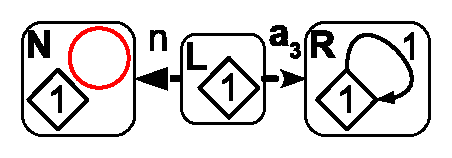
\includegraphics[scale=0.45]{images/process/order/a3}}}
    \caption{Action $a_3$}\label{fig:process:order:a3}
  \end{subfigure}%
  \begin{subfigure}[t]{.5\textwidth}
    \centerline{\fbox{\includegraphics[scale=0.45]{images/process/order/a4}}}
    \caption{Action $a_4$}\label{fig:process:order:a4}
  \end{subfigure}
  \stepcounter{doubly-typed-grammar-counter}
  \caption{Strongly safe grammar GG\arabic{doubly-typed-grammar-counter}}\label{fig:process:order}
\end{figure}

  The existential relation of this grammar is: $a_1 \leq_e a_2, a_2 \leq_e a_4, a_1 \leq_e a_4, a_3 \leq_e a_3$. Without the NACs, any sequentialization where the order $a_1 < a_2 < a_4$ is maintained would be valid, such as $[a_1, a_2, a_3, a_4]$, $[a_1,a_3,a_2,a_4]$, $[a_3, a_1, a_2, a_4]$ and $[a_1,a_2,a_4,a_3]$.

  However, as this grammar have NACs, the following conditional conflicts and dependencies have been identified:
\begin{itemize}
  \item delete-forbids: $a_4 <_{df} a_3$ caused by the deletion of $\Circle_2$.
  \item produce-forbids: $a_3 <_{pf} a_1$ caused by creation of $\Circle_1$, and $a_3 <_{pf} a_2$ caused by the creation of $\Circle_2$.
\end{itemize}

  Notice that, despite of the fact that $a_2$ deletes $\Circle_1$, which triggers the NAC of $a_3$, $a_2 <_{df} a_3$ is not a delete-forbid dependency because $a_2$ also creates $\Circle_2$, an element that still triggers the same NAC. Therefore the transformations when searching for the dependency between $a_2$ to $a_3$ are not valid.

  None of these conflicts or dependencies is \emph{concrete}, depending on how the orders are applied according to the existential relation and unconditional occurrence relation to exist.
  
  This situation is summarized in Figure~\ref{fig:process:order:cycle}, where the existential relation, the conflicts and dependencies are represented (without the explicit representation of transitivity and reflexivity). At first, if we are consider all the relations \textbf{as they are calculated}, there is no possible sequentialization for this actions, denoted by the cycle in the ordering graph.

\begin{figure}[!ht]
  \centering
  \fbox{\includegraphics[scale=0.6]{images/process/order/cycle}}
  \caption{Cycle due to conditional conflicts and dependencies}\label{fig:process:order:cycle}
\end{figure}

  Regarding the element $\Circle_1$, we have an abstract produce-forbid conflict as $a_3$ can be applied before $a_1$ creates it or after $a_2$ deletes it. Thus it is possible to apply $a_3$ as long as $a_3 \not\in [a_1\ldots a_2]$. %\mbox{$[a_3 <_{pf} a_1$ $|$ $a_2 < a_3]$}.

  As for the element $\Circle_2$, we have an abstract produce-forbid conflict \mbox{$[a_3 <_{pf} a_2$ $|$ $a_4 < a_3]$} and an abstract delete-forbid dependency \mbox{$[a_3 < a_2$ $|$ $a_4 <_{df} a_3]$}. Since the produce-forbid and the delete-forbid act on the same element, we can simply say that \mbox{$[a_3 <_{pf} a_2$ $|$ $a_4 <_{df} a_3]$}. In this configuration, $a_3$ can be applied as long as $a_3 \not\in [a_2\ldots a_4]$.

  In fact, we have that this particular grammar can be executed in any total ordering of its existential relation $a_1 \leq_e a_2, a_2 \leq_e a_4, a_1 \leq_e a_4, a_3 \leq_e a_3$ that also respects the \emph{restrictions} $a_3 \not\in [a_1\ldots a_2]$ and $a_3 \not\in [a_2\ldots a_4]$.

  There exist two such sequentializations of this existential relation: $[a_3, a_1, a_2, a_4]$ and $[a_1,a_2,a_4,a_3]$.
\end{example}

\begin{remark}[Abstract Dependencies and Conflicts] The existence of an abstract produce-forbid conflict caused by an element $x$ is conditioned to the existence of an action which deletes $x$.

  Given an action $a_1$ which creates $x$, an action $a_2$ whose NAC forbids $x$ and provided a configuration where $a_1$ was applied before $a_2$, we have that $a_2$ can be applied only after an action $a_3$ which deletes $x$ has been applied.

  However, $a_3$ may also cause a new produce-forbid conflict on $a_2$ by creating a new element $y$ which is also forbidden by a NAC of $a_2$, on which case $a_2$ can only be applied of there is another action $a_4$ which ``turns off'' the conflict caused by $a_3$.

  In general, for each abstract produce-forbid conflict $a_2 <_{pf} a_1$ caused by an element $x$, we have that $a_2$ must be successfully applied before $a_1$ or after an action $a_{j}$ where $a_i$ deletes $x$ and $a_i \leq a_j$.

  Analogously, for each abstract delete-forbid conflict $a_1 <_{df} a_2$ caused by an element $x$, we have that $a_2$ must be successfully applied after $a_1$ or before an action $a_j$ where $a_i$ creates $x$ and $a_j \leq a_i$.
\end{remark}

\begin{definition}[Occurence Relation] Given a strongly safe grammar \doublyTypedGraphGrammarCore{}, let $[\leq_{df}]$ be the set of all its \emph{concrete} delete-forbids and $[\leq_{pf}]$ be the set of all its \emph{concrete} produce-forbids. Then, its occurrence relation $\leq_o$ of $(P \cup N(C^T) \cup E(C^T))$ is defined as the transitive and reflexive closure of \mbox{$\leq_{e}$ $\cup$ $[\leq_{df}]$ $\cup$ $[\leq_{pf}]$}.
\end{definition}

\begin{definition}[Occurence Relation Restrictions] Given a strongly safe grammar \doublyTypedGraphGrammarCore{}, its \emph{occurence relation restrictions} is the set $R$ containing all its abstract produce-forbid conflicts and delete-forbid dependencies.
\end{definition}

\begin{definition}[Occurrence Graph Grammars] Let \doublyTypedGraphGrammarCore{} be a strongly safe graph grammar. $GG$ is an \emph{occurrence graph grammar} iff:

  \begin{enumerate}
    %\item acyclic existential relation: $\forall a \in P$: $\leq_e$ is antisymmetric;
    \item acyclic occurrence relation: $\forall a \in P$: $\leq_o$ is antisymmetric;
    \item there is at least one serialization of the actions $a_1,\ldots,a_n \in P$ that respects the occurrence relation restrictions.
  \end{enumerate}
\end{definition}

As was said in the beginning of this chapter, the idea is that an occurrence graph grammar is a suitable to describe the semantics of a graph grammar, in the sense that it represents both all possible states and changes of states that is also a graph grammar.

The first condition of the definition assures that it is possible to find a sequence of actions that respects both the order of creation and deletion of elements given by the existential relation and the order imposed by the concrete produce-forbids and delete-forbids of the grammar. In other words, it assures that there is no cycle of conflicts and dependencies that can prevent the application of the grammar.

The second condition deals with the conflicts and dependencies induced by NACs that do not participate in the concrete relations and generate \emph{intervals} of actions in which specific inside of which specific actions can not be applied.


\begin{definition}[Concurrent Graphs] Given \doublyTypedGraphGrammarCore{} an occurrence graph grammar and $G$ a subgraph of \coreGraph{}. Let \mbox{$A = \{a \in P | a\in Pre^{\leq_o}(x) \land x \in G\}$}. Then $G$ is a \emph{concurrent graph} iff the following conditions are satisfied for all $x,y \in G$:

\begin{enumerate}
  \item $x \not\leq_o y \land y \not\leq_o x$
  \item $x$ satisfies the occurrence restrictions for elements
\end{enumerate}

\end{definition}


\chapter{Verigraph Tool Overview}\label{ch:verigraph}

Verigraph~\cite{verigraph} is a new tool for simulating and analizing graph grammars implemented in Haskell\footnote{The source code is available at \url{https://github.com/Verites/verigraph}}, a purely functional programming language. The tool is being developed by the Verites group\footnote{\url{http://www.ufrgs.br/verites}} with two particular aims. The first one is to build a software tool that serves as an implementation of standard constructions and analysis for graph grammars, while also being as closely related to the theory as possible. The second, to provide a framework for exploring new ideas and techniques in graph grammars and other category theory related topics~\cite{BezerraETMF2016,Costa2016,CostaETMF2016, Becker2014}.

Regarding category theory, Verigraph implements important basic constructions such as coequalizers, coproducts, colimits, pushout complements, initial pushouts, pullbacks, negative application conditions, constraints, among others. The implementation of this constructions follows a very similar approach to the one used in~\cite{Rydeheard1988}, where categorial concepts are implemented as types in ML and constructive proofs of theorems in category theory are built as ML programs.

The implemented categorial constructions are used as a basis to implement several graph grammar analyses, such as critical pair analysis~\cite{Lambers2006}, state space generation and model checking~\cite{Becker2014}, concurrent rules generation~\cite{BezerraETMF2016} and higher-order graph transformations~\cite{Machado2015}. They were also used to implement the construction of occurrence graph grammars with NACs, which were explained in depth in chapter~\ref{ch:process}.

The analysis algorithms are implemented in a generic functional style, having the advantage of being very close to the formal definitions, thus making it easier to reason about them and to inspect for correctness. 
In addition, Verigraph benefits from a layered architecture, shown on Figure~\ref{fig:verigraph:layers}, where it is easy to reuse the same analysis algorithms (top layer) for other categories different than \cat{TGraph_T} (bottom layer), as long as they implement the contracts given
by the type classes (middle layer) defined on the system.
Examples of these type classes are shown on Figures~\ref{fig:verigraph:morphism-type-class} and \ref{fig:verigraph:cocomplete-type-class}.

\begin{figure}[!ht]
  \centering
  \begin{subfigure}[t]{.5\textwidth}
    \centerline{\includegraphics[scale=0.6]{images/verigraph/layers}}
%    \caption{Detailed Layers}
  \end{subfigure}
%  \begin{subfigure}[t]{.5\textwidth}
%    \centerline{\includegraphics[scale=0.5]{images/verigraph/layers-abstract}}
%    \caption{Example}
%  \end{subfigure}%
  \caption{Verigraph architecture}\label{fig:verigraph:layers}
\end{figure}

There are tools for analysing graph grammars which are similar to Verigraph in some aspects, such as AGG~\cite{Taentzer2000} and GROOVE~\cite{Rensink2004}. Recently, \cite{Deckwerth2016} introduced a java framework for static verification of graph transformations also based in category theory.
  However, to our knowledge, Verigraph is the only tool that integrates static and dynamic analyses, second-order specifications and provides support for new categorial constructions and algorithms, besides being the only tool in this field implemented in a pure functional language~\cite{Costa2016}.
  Moreover, Verigraph is a free and open source software, available online for the community in one of the biggest platforms for software repositories currently available. In addition to it, not only its source code, but also its roadmap are public and open to suggestions and collaborations from outside the Verites group.

In the next sections of this chapter, we will demonstrate basic aspects of Verigraph implementation. First we present general categorial constructions which are the basic foundations of the tool; then we provide details about the implementation of concrete objects and categories, specifically focusing on \typedGraphCategory{}; after, we present the implementation of some analysis algorithms and show how they can be reused by other categories. %Finally, we explain in depth how the calculation of Occurrence Graph Grammars was implemented, which is part of our thesis contribution.

\section{Implementation of Categorial Constructions}

The first basic type class in Verigraph is \code{Morphism}, shown in Figure~\ref{fig:verigraph:morphism-type-class}, which serves as the minimal contract for any category to be implemented in the tool. Notice how the contract of this type class reflects the category definition (see Definition~\ref{def:category}).

\begin{figure}[!ht]
\caption{Morphism Type Class}
\begin{minted}[linenos=true, breaklines,fontsize=\small]{haskell}
class (Eq m) => Morphism m where
    type Obj m :: *
    compose  :: m -> m -> m
    domain   :: m -> Obj m
    codomain :: m -> Obj m
    id       :: Obj m -> m
    isMonomorphism :: m -> Bool
    isEpimorphism :: m -> Bool
    isIsomorphism :: m -> Bool
\end{minted}
\label{fig:verigraph:morphism-type-class}
\end{figure}

All the other type classes in the tool that are related to category theory are somehow defined in terms of \code{Morphism}. For example, the \code{Cocomplete} type class shown in Figure~\ref{fig:verigraph:cocomplete-type-class} defines some of the most basic categorial constructions used in Verigraph, such as coequalizers, coproducts and pushouts.

Notice that in the \code{Cocomplete} definition any category that implements the functions \code{calculateCoequalizer} and \code{calculateCoproduct} automatically will have a standard implementation of the \code{calculatePushout} function based only on these two constructions. This is due to the fact that, whenever a category has coequalizers and coproducts, it is possible to calculate any (finite) colimit based only on these two constructions, as demonstrated in~\cite{Pierce1991}.

We took advantage of this result to implement not only the \code{calculatePushout}, but also the calculation of the \code{colimit} of a diagram. The later being used in the generation of occurrence graph grammars as will be shown in chapter~\ref{ch:tests}.

Another interesting characteristic of the \code{Morphism} type class is that, even though \code{pushouts} and \code{colimits} are implemented in terms of \code{coproducts} and \code{coequalizers}, the programmer can override the default implementation and provide his/her own (categorial specific) implementation. This could be useful, for example, when for a given category \cat{C}, a particular algorithm to calculate the pushout is known to be more optimized than using the composition of basic operations.

\begin{figure}[!ht]
  \begin{minted}[linenos=true, breaklines, fontsize=\small]{haskell}
class (Morphism m) => Cocomplete m where
  calculateCoequalizer :: m -> m -> m
  calculateNCoequalizer :: NonEmpty m -> m
  calculateCoproduct :: Obj m -> Obj m -> (m,m)
  calculateNCoproduct :: NonEmpty (Obj m) -> [m]

  calculatePushout :: m -> m -> (m, m)
  calculatePushout f g = (f', g')
    where
      b = codomain f
      c = codomain g
      (b',c') = calculateCoproduct b c
      gc' = compose g c'
      fb' = compose f b'
      h = calculateCoequalizer fb' gc'
      g' = compose b' h
      f' = compose c' h
\end{minted}
\caption{Cocomplete Type Class}\label{fig:verigraph:cocomplete-type-class}
\end{figure}

In addition to \code{Morphism}, Verigraph has several other important type classes, some examples are:
\begin{itemize}
  \item \code{FindMorphism} for finding morphisms between objects of a category;
  \item \code{AdhesiveHLR} for operations that AdhesiveHLR categories (e.g. \cat{TGraph_T}) are guaranteed to have, such as calculating initial pushouts and pushout complements (when they exist);
  \item \code{DPO} for operations related to DPO graph rewriting approach, such as inversion of rules.
\end{itemize}

As for the concrete categories used, currently there are three specific implementations in Verigraph. Besides \cat{Graph} and \cat{TGraph_T}, which were reviewed on chapter~\ref{ch:gts}, there is also an implementation of \cat{TSpan_T}, where we have $T-$typed graph morphism spans are objects and span morphisms are arrows or, from a more concrete perspective, DPO graph rules as objects and morphisms between rules as arrows.

\section{Implementation of Graph Grammars}

The main concrete structures in Verigraph are (typed) graph grammars, which is currently the focus of the Verites group. The basic implementation begins with the \code{Graph} type, which consists of a list of nodes and a list of edges together with an API for graph manipulation with basic functions.

The \code{Graph} definition on Haskell is show on Figure~\ref{fig:verigraph:graph}. The \code{Graph} API is not shown, but it includes basic graph operations such as \code{insertNode}, \code{insertEdge}, \code{removeNode}, \code{removeEdge}, \code{incomingEdges}, \code{outgoinEdges}, \code{sourceOf}, \code{targetOf}, among others. 

\begin{figure}[!ht]

\caption{Graph implementation}
\begin{minted}[linenos=true, breaklines,fontsize=\small]{haskell}
data Node a = Node 
{ getNodePayload :: Maybe a
}

data Edge a = Edge 
{ getSource      :: NodeId
, getTarget      :: NodeId
, getEdgePayload :: Maybe a
}

data Graph a b = Graph 
{ nodeMap :: [(NodeId, Node a)]
, edgeMap :: [(EdgeId, Edge b)]
}
\end{minted}
\label{fig:verigraph:graph}
\end{figure}

We use \code{Graph} to progressively build the morphisms necessary to implement the categories \cat{Graph}, \cat{TGraph_T} and \cat{TSpan_T}. A graph morphism consists of a graph as domain, a graph as codomain and relations that map the nodes and edges in the domain graph to the ones in the codomain one. A typed graph is regarded as a simple graph morphism and a typed graph morphism consists of a typed graph as domain, a typed graph as codomain and a graph morphism relating the two of them.

Figure~\ref{fig:verigraph:concrete-morphisms} shows all categories currently implemented in Verigraph based on their morphisms. Moreover, all concrete morphisms presented implement the \code{Morphism} type class. Figure~\ref{fig:verigraph:morphism-implementation} shows how \code{TypedGraphMorphism} implements \code{Morphism} type class in order to provide the \cat{TGraph_T} category.

Similar implementations were done for \code{GraphMorphism} and \code{RuleMorphism}.

\begin{figure}[!ht]
\caption{Basic concrete morphisms of Verigraph.}
\begin{minted}[linenos=true, breaklines,fontsize=\small]{haskell}
data GraphMorphism a b = GraphMorphism 
{ getDomain    :: Graph a b
, getCodomain  :: Graph a b
, nodeRelation :: R.Relation G.NodeId
, edgeRelation :: R.Relation G.EdgeId
}

type TypedGraph a b = GraphMorphism a b

data TypedGraphMorphism a b = TypedGraphMorphism 
{ getDomain   :: TypedGraph a b
, getCodomain :: TypedGraph a b
, mapping     :: GraphMorphism a b
}

data RuleMorphism a b = RuleMorphism 
{ rmDomain         :: Production (TypedGraphMorphism a b)
, rmCodomain       :: Production (TypedGraphMorphism a b)
, mappingLeft      :: TypedGraphMorphism a b
, mappingInterface :: TypedGraphMorphism a b
, mappingRight     :: TypedGraphMorphism a b
}
\end{minted}
\label{fig:verigraph:concrete-morphisms}
\end{figure}

\begin{figure}[!ht]
\caption{Typed graph morphism implementing morphism type class.}
\begin{minted}[linenos=true, breaklines,fontsize=\small]{haskell}
instance Morphism (TypedGraphMorphism a b) where
  type Obj (TypedGraphMorphism a b) = TypedGraph a b
  domain = getDomain
  codomain = getCodomain
  compose t1 t2 = TypedGraphMorphism (domain t1) (codomain t2) $ compose (mapping t1) (mapping t2)
  id t = TypedGraphMorphism t t (M.id $ domain t)
  isMonomorphism = isMonomorphism . mapping
  isEpimorphism = isEpimorphism . mapping
  isIsomorphism = isIsomorphism . mapping
\end{minted}
\label{fig:verigraph:morphism-implementation}
\end{figure}

\section{Implementation of the Analysis Algorithms}

The analysis algorithms are also implemented at a high level of abstraction, based on categorial definitions and their implementation as type classes. For example, the code for calculating conflicts or dependencies between two rules was first implemented for \cat{TGraph_T}, but since it is based on the abstraction of \code{DPO} type class this piece of code can be reused by any other category implementing the \code{DPO} contract.

Furthermore, Figure~\ref{fig:verigraph:delete-use-produce-use} shows a piece of code with functions responsible to test whether an overlapping pair of two rules rises a conflict or a dependency for one of those rules. Notice how this code resembles the definitions of delete-use conflict (Definition~\ref{def:classic-conflict}) and produce-use dependency (Definition~\ref{def:classic-dependency}).


\begin{figure}[!ht]
\caption{Delete-Use and Produce-Use Implementation}
\begin{minted}[linenos=true, breaklines,fontsize=\small]{haskell}
-- | Rule @p1@ is in a delete-use conflict with @p2@ if @p1@ deletes something that is used by @p2@. This function verifies the non existence of h21: L2 -> D1 such that d1 . h21 = m2
isDeleteUse :: (DPO m) => Production m -> (m, m) -> Bool
isDeleteUse p1 (m1,m2) = null h21
  where
    --gets only the morphism d1 from D1 to G
    (_,d1) = calculatePushoutComplement m1 (getLHS p1) 
    h21 = findAllPossibleH21 m2 d1

isProduceUse :: (DPO m) => Production m -> (m, m) -> Bool
isProduceUse p1 (m1',m2) = null h21
  where
   --gets only the morphism d1 from D1 to G
   (_,e1) = calculatePushoutComplement m1' (getRHS p1)
   h21 = findAllPossibleH21 m2 e1
\end{minted}
\label{fig:verigraph:delete-use-produce-use}
\end{figure}

As an example of its application at other categories we have \cat{TSpan_T}, which also implements the \code{DPO} type class and benefits from the same algorithms for finding conflicts and dependencies. This also can be used for different categories based on graphs, algebras, logics and so on.

Besides basic categorial constructions and several analysis techniques for graph grammars, Verigraph was also used to implement the construction of Occurrence Graph Grammars and the relations presented in chapter~\ref{ch:process}. This construction is presented in more detail in the following chapter.



\chapter{Construction of Occurrence Graph Grammars}\label{ch:tests}

%A test case is a collection of (1) input values necessary to complete some execution of the system under testing, (2) the results that must be produced after executing the test (assuming the system satisfies the intended behaviour) and (3) any inputs necessary to setup the system into the appropriate state to receive the test values~\cite{Ammann2008}.
%Test oracles are specifications describing properties about the validity of tests cases, i.e. if the test must fail or pass. These properties may include relationships between the input given and the expected output, data validity properties, format of possible execution paths, etc. No matter the oracle format, it must be able to determine the validity of tests in a finite and reasonable amount of time~\cite{Weyuker1982}.

%In the following, we show how to use \newadd{deterministic} occurrence graph grammars to generate test cases and oracles from (simply-typed) graph grammars modelling systems. In theory, this approach can be used to generate tests for any graph grammar\footnote{\newadd{Assuming the grammar follows the DPO approach with incremental NACs}}, since it is based only on the properties of the formalism. However, we focused on graph grammars that were generated from use cases by using the methodology presented in \cite{Junior2015}, \cite{BezerraWEIT2016} and \cite{Cota2017}.

%This methodology is a systematic, computer-aided way to extract graph grammars from use cases or other text-based requirement documents. At the same time, it helps finding problems such as ambiguities, inconsistencies and omissions in the documents. Thus, providing a better specification and also an improved model. By generating tests from these grammars we are indirectly generating tests for the underlying use cases. The test generation, to be described in next sections, was implemented in Verigraph as an extension of the previously discussed calculation of occurrence graph grammars.

%We focused our approach on testing the integration of different functionalities (or requirements) of a system. By \emph{functionality}, we informally mean an aim the system is supposed to accomplish, which has value to a user or any other stakeholder. By \emph{integration} we mean the emergent behaviour of executing several functionalities, possibly multiple times.

% In the graph grammar model of a system, a functionality can be represented either as a single rule or as a collection of rules. In either case, those rules must be executed to achieve the functionality goals. Therefore, the main idea of our approach is that, given a collection of functionalities, we find out whether it is possible to find a sequence in which all these functionalities can be performed, then we characterize the assumptions that must be satisfied for them to be performed and/or the restrictions that may prevent their execution. Given a collection of functionalities modelled as graph rules, we are interested in generating:

\iffalse
\begin{enumerate}
\item the minimal input data necessary for these functionalities to execute, as well as the output data of a successful execution;
\item at least one path in which all functionalities can be applied (if possible);
\item a set of constraints two characterize any test into those which should pass and those which should fail;

\hide{
\item a set of constraints which can tell which intermediate states of the system are valid and those that are not.}
\end{enumerate}

Notice that the two first items correspond to test cases while the last one correspond to test oracles.
\fi
%First, we present a brief overview of the methodology for extracting graph grammars from use cases, after what we present the process of generating the tests cases from the extracted grammars.

In this chapter, we present the process of constructing Occurrence Graph Grammars with NACs (OGGs) in a systematic manner and how this process was implemented in Verigraph. We use the same grammar presented on Example~\ref{ex:mail-grammar} in order to illustrate the explanation. We also applied this process in more complex graph grammars. One of the grammars models the system of a restaurant, with functionalities such as login of employees, reservation and cancellation of tables,
accommodation of clients, serving tables, among others. Another models the system of an e-Store, with functionalities such as browse and search catalogue, registration of clients, login, maintain shopping cart, effectuate purchase, etc. The grammars, their textual specifications (use cases), together with their generated OGGs can be found at the Verites repository for case studies\footnote{https://github.com/Verites/case-studies}.



%that modelling the system of a restaurant and , built from the set of use cases presented in Appendix~\ref{app:use-cases} by applying the systematic methodology proposed by~\cite{Junior2015}. These use cases model basic functionalities of the proposed restaurant system such as login of employees, reservation and cancellation of tables, accommodation of clients, serving tables, among others. The complete extracted grammar, together with its generated OGGs can be found at the Verites repository for case studies\footnote{https://github.com/Verites/case-studies}.

First, we reintroduce the \emph{Mail Server Graph Grammar}, then we proceed to the explanation of the necessary steps to build an Occurrence Graph Grammar according to the definitions presented on chapter~\ref{ch:process}. The implementation of this process in Verigraph is also part of this thesis contribution, as Verigraph is the first tool in the field to implement the construction of Occurrence Graph Grammars, even when considering OGGs without NACs. As a possible practical application of this, at the end of the chapter, we provide some insight about how OGGs can be used to generate test cases for the system they model.
%Given the graph grammar model of a system, we want to generate test cases and oracles for collections of its underlying functionalities. These collections could represent something as ``atomic'' as a successful or failing login attempt or something as complex as the entire workflow of attending clients, which would require attendants and waiters to log in into the system, tables to be occupied, orders to be prepared, among possibly several other steps.

%The reason why we focused on collections of functionalities is to test the emergent behaviour of a system, which usually is not observable if we consider each functionality in isolation. By grouping together several (usually, but not necessarily different) functionalities, we may realize how they interact with each other and which are the overall effects of this integration.

%\begin{definition}[Functionality Collection] Given a graph grammar \graphGrammar{} that models a system, a \emph{functionality collection} $F$ is a collection of its grammar rules. The term collection here is used instead of set to imply that the same rule $r \in P$ can appear more than once in $F$. In this context, it means the functionality modelled by $r$ is intended to be executed more than once.
%\end{definition}

%\section{Running Example}

\begin{example} %The rules we chose for this example represent one way in which the entire process of serving a client can be accomplished. In this particular case, we chose the rules representing the successful paths of the use cases \emph{reserve table}, \emph{accommodate client}, \emph{serve table} and \emph{close table}, which are depicted on figure~\ref{fig:tests:grammar}.
  The grammar used here illustrates a mail server scenario for a simple e-mail application composed by four rules, which are described in the following and depicted in Figure~\ref{fig:tests:grammar}.
  In order to better present the ideas of this chapter in terms of its implementation, we use the rules in the format provided by AGG~\cite{Taentzer2000}, which is also the format used as input and output by Verigraph.
  This format depicts the LHS and RHS graphs of rules, but does not explicitly show the interface graph, which can be inferred by identification numbers correlating items of LHS and RHS.

\begin{enumerate}[label=(\alph*),start=1]
  \item \emph{Send message:} a client writes a message which they send to a server, however there is a NAC forbidding the message of being sent if it has a piece of data attached to it.
  \item \emph{Get data:} a piece of data is obtained from a server and attached to a message.
  \item \emph{Receive message:} a server sends a message with attached data to a client.
  \item \emph{Delete message:} a client obtains a piece of data from a received message and this message is destroyed.
\end{enumerate}
\end{example}
%
%\begin{description}
%  \item[Reserve table:] A receptionist of the restaurant tags a table as reserved for a specific client at a given date and time. Therefore, this table must not be allocated for another client, either by accommodation or reservation, at the same time.
%  \item[Accomodate client without reservation:] A receptionist leads a client to a free table, then notifies the system that this table is waiting for service.
%  \item[Serve table:] A waiter goes to an occupied table to take an order, adding or removing items to/from the order, then closing it and sending it to the kitchen to be prepared.
%  \item[Close table:] A waiter goes to a table that has been serviced, closes the corresponding bill and collects the payment from its client.
%\end{description}

\begin{figure}[!ht]
  \centering
  \begin{subfigure}[t]{.5\textwidth}
    \centerline{\fbox{\includegraphics[scale=0.5]{grammar/server/sendMsg}}}
    \caption{Rule \emph{send message}}
  \end{subfigure}
  \begin{subfigure}[t]{.5\textwidth}
    \centerline{\fbox{\includegraphics[scale=0.5]{grammar/server/getData}}}
    \caption{Rule \emph{get data}}
  \end{subfigure}
  \begin{subfigure}[t]{.5\textwidth}
    \centerline{\fbox{\includegraphics[scale=0.5]{grammar/server/receiveMsg}}}
    \caption{Rule \emph{receive message}}
  \end{subfigure}
  \begin{subfigure}[t]{.5\textwidth}
    \centerline{\fbox{\includegraphics[scale=0.5]{grammar/server/deleteMsg}}}
    \caption{Rule \emph{delete message}}
  \end{subfigure}
  \caption{Rules for a mail server application}\label{fig:tests:grammar}
\end{figure}

\section{Selecting a Computation of GG}

  In this work we defined only deterministic Occurrence Graph Grammars with NACs, and therefore, in contrast to~\cite{Ribeiro1996}, where the semantics of a Graph Grammar is represented by only one (non-deterministic) Occurrence Graph Grammar, here we need a set of Occurrence Graph Grammars to represent the behaviour of a Graph Grammar.
  Nevertheless, this set is usually much smaller than the set of all derivations of a Graph Grammar since each OGG represents a (shift-)equivalent set of derivations, that is, a set of derivations that are equivalent with respect to switching the order of independent steps. 
  In the following we will describe how to construct one OGG, the complete behaviour of a GG would be described by the (possibly infinite) set of OGGs that can be constructed with the rules of the underlying GG. Note that, even in the case of~\cite{Ribeiro1996}, where the semantics was described by only one OGG, this structure may be  infinite in the case the system has the possibility of a non-terminating computation.

  Thus, in order to construct an Occurrence Graph Grammar $OGG$ for a graph grammar \graphGrammar{}, we need (1) a collection\footnote{ We use the term collection instead of set because, in this case, a rule can appear more than once since each rule in $F$ represents the application of a rule in $P$.} of rules $F$ based on $P$, which represent the rules that are applied in the computation depicted by the OGG, and (2) a way of specifying how the rules in $F$ interact among themselves. 
  The latter is needed to define which elements are common throughout the rules. To this purpose, we use an \emph{input-output relation}, depicting connections between the rules in $F$.
  The objects in this relation identify which elements must be the same between pairs of rules.
  This construction is similar to the construction of concurrent rules in AGG.
  The difference is that instead of building a rule, the result of our construction is an OGG, i.e., represents a computation.

\begin{definition}[Input-Output Relation] Given a collection $F$ of rules, an \emph{input-output relation} $IO$ over $F$ is a set of typed-graph morphism spans of the form \mbox{$R_x \leftarrow IO_i \rightarrow L_y$} each of which connects two distinct rules $x,y \in F$.

\end{definition}

The $IO_i$ object of each span works similarly to the gluing graph $K$ of a rule, but instead of identifying elements that are the same in both left and right sides of a single rule, it identifies elements that are necessarily the same between the right and left sides of two different rules. An input-output relation for a collection of rules will have an appearance similar to the following diagram, where there are several $IO$ objects connecting the right-hand side of a rule with the left-hand side of another one.

\diagram{
  & & & & IO_6\ar@{-->}[dddrrrr]\ar@{-->}[dddllll] & & & &\\
  & IO_3\ar@{-->}[ddl]\ar@{-->}[ddrrrr] & & & & & & IO_4\ar@{-->}[ddr]\ar@{-->}[ddllll] &\\
  & & IO_1\ar@{-->}[d]\ar@{-->}[dr] & & IO_5\ar@{-->}[drr]\ar@{-->}[dll] & & IO_2\ar@{-->}[d]\ar@{-->}[dl] & &\\
  L_1 & K_1\ar[l]\ar[r] & R_1 & L_2 & K_2\ar[l]\ar[r] & R_2 & L_3 & K_3\ar[l]\ar[r] & R_3\\
  }


\begin{remark}We could have have also included in the $IO$ relation a type of span that also connects only the left (resp. right) sides of rules together, however we would accomplish very little with this kind of span. Given that we are looking for Occurrence Graph Grammars, where the exact same element can not be deleted or created by two different rules, this particular kind of span would serve only to identify elements that are preserved by both rules, otherwise they would introduce inconsistencies, therefore preventing the creation of OGGs.
\end{remark}

\begin{example}[Input-Output Relations]\label{ex:inout} Figure~\ref{fig:tests:inout} shows one possible $IO$ relation for our running example. Notice that the elements which should be the same in both rules have the same prefix number in their identification. The first $IO$ object connects the rules \emph{send message} and \emph{get data}.  In this case, we want the server, the message and the connection between them to be the same in both rules. %For example, the table involved in both action is the same table, as a client there is accommodated must also be served. The employees, on the other hand, are not, as the employee who receives the client in the restaurant (the receptionist) is not the same who serves the client (the waiter).

As a side note, the reader may notice that it is not mandatory to create an $IO$ span \mbox{$\left(R_x \leftarrow IO_i \rightarrow L_y\right)$} for \textbf{every} pair of rules. For example, consider that we want to analyse a scenario where the \emph{server} node is unique. Given rules \emph{get data} and \emph{receive message}, we have the options of building the span that identifies the server node as
  $R_{sendMsg} \leftarrow IO_n \rightarrow L_{receiveMsg}$ or $R_{receiveMsg} \leftarrow IO_m \rightarrow L_{sendMsg}$, or even the two of them. Any combination would result in the same final effect: both rules use the same \emph{server}.
  \begin{figure}[!ht]
  \centering
  \fbox{\includegraphics[scale=0.5]{grammar/server/io-object}}
  \fbox{\includegraphics[scale=0.5]{grammar/server/io-object2}}
  \fbox{\includegraphics[scale=0.5]{grammar/server/io-object3}}
  \caption{A basic Input-Output relation building}\label{fig:tests:inout}
\end{figure}

\end{example}

Currently, the generation of the \textit{input-output relation} is a manual step in our strategy, therefore the analyst needs to decide how to better implement his/her own $IO$ relation. This did not shown to be a problem, as in our analysis we usually wanted to restrict the number of possible combinations to more realistic cases. However, its fully automation was scheduled as future work.


\section{Constructing the OGG}

  Having $GG$, the graph grammar model of the system; $F$, a collection of rules; and $IO$, an \emph{input-output relation}, we proceed to the construction of an occurrence graph grammar for $GG$ accomplished by means of an amalgamation of $F$ over its input-output relation $IO$.
  This amalgamation is later used in the construction of a doubly-typed graph grammar, which we then check to verify whether it satisfies the conditions to be an occurrence grammar. The construction steps are specified in
  Definition~\ref{def:ogg-construction}, which is an adaptation of the construction of an occurrence graph grammar without NACs from~\cite{Corradini1996}.

\begin{definition}[Deterministic Occurrence Graph Grammar Construction]\label{def:ogg-construction} Given a grammar \graphGrammar{}, $F$ a collection of rules from $P$, and $IO$ and input-output relation over the rules in $F$:

\begin{enumerate}
  \item\label{enum:construction-colimit} calculate the amalgamation (colimit) $Occ$ of the rules in $F$ with respect to $IO$ as presented in the following diagram, where all squares commute.

\diagram{
  & & & & IO_6\ar[dddrrrr]\ar[dddllll] & & & & \\
    & IO_3\ar[ddl]\ar[ddrrrr] & & & & & & IO_4\ar[ddr]\ar[ddllll] &\\
    & & IO_1\ar[d]\ar[dr] & & IO_5\ar[drr]\ar[dll] & & I O_2\ar[d]\ar[dl] & &\\
    L_1\ar[dddrrrr] & K_1\ar[l]\ar[r] & R_1\ar[dddrr] & L_2\ar[dddr] & K_2\ar[l]\ar[r] & R_2\ar[dddl] & L_3\ar[dddll] & K_3\ar[l]\ar[r] & R_3\ar[dddllll]\\
    & & & & & & & &\\
    & & & & & & & &\\
    & & & & Occ & & & &
}\hfill\break

\hide{
\diagram{
  & & & & IO_6\ar[dddrrrr]\ar[dddllll] & & & & &\ldots\\
    & IO_3\ar[ddl]\ar[ddrrrr] & & & & & & IO_4\ar[ddr]\ar[ddllll] & & \ldots\\
    & & IO_1\ar[d]\ar[dr] & & IO_5\ar[drr]\ar[dll] & & IO_2\ar[d]\ar[dl] & & &\ldots\\
    L_1\ar[dddrrrr] & K_1\ar[l]\ar[r] & R_1\ar[dddrr] & L_2\ar[dddr] & K_2\ar[l]\ar[r] & R_2\ar[dddl] & L_3\ar[dddll] & K_3\ar[l]\ar[r] & R_3\ar[dddllll] & \ldots\ar[dddlllll]\\
    & & & & & & & & &\\
    & & & & & & & & &\\
    & & & & Occ & & & & &
}\hfill\break}

\item \emph{retype} the rules in $F$ over $Occ$: use each morphism found from each $L_i, K_i, R_i$ to $Occ$ as their respective new typing morphism. This step generates a set $F'$ of doubly-typed graph rules, given that $Occ$ is a $TG$-typed graph itself.

\item calculate the causal relation $\leq_{c}$ of the doubly-typed graph rules in $F'$.

\item\label{enum:construction-graphs} generate the initial and final graphs $I$ and $J$ by respectively deleting from $Occ$ all elements ever created and deleted by the rules in $F'$.

\item\label{enum:construction-occurrence} calculate and categorize the produce-forbid conflicts and delete-forbid dependencies according to definitions~\ref{def:delete-forbid-strong} and~\ref{def:produce-forbid-strong}.

\begin{enumerate}
\item\label{enum:construction-analysis} use the concrete conflicts and dependencies to extend the causal relation in order to obtain the occurrence relation $\leq_o$.

\item\label{enum:construction-restriction} use the abstract conflicts and dependencies to generate the set $R$ of restrictions over the ordering of rules applicability.
\end{enumerate}

\item\label{enum:construction-ordering} find one or more total orderings of rules in $F'$ which respects both the occurrence relation and the occurrence restrictions.
\end{enumerate}

%  The (Deterministic) Occurrence Graph Grammar representing execution of the functionality $i$ is given by $OGG_i = (Occ_i, I_i,F_i)$, iff $OGG_i$ respects the conditions imposed by Definition~\ref{def:ogg} 
\end{definition}

If all the steps in such a construction can be successfully executed, specially steps~\ref{enum:construction-graphs} and~\ref{enum:construction-ordering}, we have that $OGG = (Occ, I, F')$ is not only a doubly-typed graph grammar, but also a deterministic occurrence graph grammar. %This means it is possible to successfully apply all the rules in the original collection $F$. %Our approach creates test cases and oracles from $OGG$ whether it is in fact an occurrence graph grammar or not. In the first case, we have tests for success and failure execution paths, whereas in the second we have tests only for the failure ones. Notwithstanding, we regard the failure tests as important because they pinpoint uses of the underlying system where the system itself is supposed to fail, therefore they can not or should not be performed. In the following, we dive into details of each construction step.

The first step of the construction, the amalgamation of rules in $F$ w.r.t. $IO$, is responsible to ``glue'' the graphs of all rules in one typed graph $Occ$, while identifying the items that are meant to be the same throughout the grammar execution. This can be regarded as a mapping which turns generic elements such as \textit{a user} into concrete elements such as the user named \textit{Bob}. It also discriminates these elements, for instance: the user \textit{Bob} is different from the user
\textit{Alice}. Therefore, at the end of this step, $Occ$ contains all concrete elements ever to be created, preserved or deleted by any of the rules in collection $F$. Figure~\ref{fig:tests:amalgamation} shows the amalgamation of an $F$ containing one copy of each rule in our example grammar w.r.t. the IO relation depicted on Figure~\ref{fig:tests:inout}.

\begin{figure}[!ht]
  \centering
  \fbox{\includegraphics[scale=0.5]{grammar/server/amalgamation}}
  \caption{Amalgamation (colimit) of rules according to the basic IO relation.}\label{fig:tests:amalgamation}
\end{figure}

The retyping step is responsible for generating actions: ``new'' graph rules which, rather than being generic descriptions of system transformations, represent concrete executions of the original rules over a given context. Therefore, a rule which describes the process where a user receives from the server a message sent by another\footnote{Notice that the original graph grammar does not specify that the sender must be different from the receiver, therefore we would be able to choose a
computation where they are the same user.} user becomes a concrete action where \textit{Alice} receives \textit{the message} sent by \textit{Bob}.
%The set $F'$ of doubly-typed graph rules from the colimit calculated in the previous step.
For each graph rule $\mbox{$p_i^{TG} = \left(L_i^{TG} \leftarrow K_i^{TG} \rightarrow R_i^{TG}\right)$} \in F$, we generate a new action \mbox{$q_i^{Occ} = \left(L_i^{Occ} \leftarrow K_i^{Occ} \rightarrow R_i^{Occ}\right) \in F'$}, where the typing morphisms are those from the original rules in $F$ to the colimit graph $Occ$. Since $Occ$ is the type graph of the new rules and, at the same time, a typed graph over $TG$, the actions are now doubly-typed rules over $Occ^{TG^T}$.
Figure~\ref{fig:tests:actions} shows the actions generated for our running example\footnote{ Since we use AGG as our form of output visualization and it was not intended to provide support for doubly-typed graph grammars, the NACs of our actions can not be properly seen, however they are maintained and used in Verigraph internal format.}.

\begin{figure}[!ht]
  \centering
  \begin{subfigure}[t]{.5\textwidth}
    \centerline{\fbox{\includegraphics[scale=0.5]{grammar/server/amalgamation/sendMsg}}}
    \caption{Rule \emph{send message}}
  \end{subfigure}
  \begin{subfigure}[t]{.5\textwidth}
    \centerline{\fbox{\includegraphics[scale=0.5]{grammar/server/amalgamation/getData}}}
    \caption{Rule \emph{get data}}
  \end{subfigure}
  \begin{subfigure}[t]{.5\textwidth}
    \centerline{\fbox{\includegraphics[scale=0.5]{grammar/server/amalgamation/receiveMsg}}}
    \caption{Rule \emph{receive message}}
  \end{subfigure}
  \begin{subfigure}[t]{.5\textwidth}
    \centerline{\fbox{\includegraphics[scale=0.5]{grammar/server/amalgamation/deleteMsg}}}
    \caption{Rule \emph{delete message}}
  \end{subfigure}
  \caption{The set of actions generated w.r.t. our basic $IO$ relation}\label{fig:tests:actions}
\end{figure}

Once the set $F'$ of actions was created, we proceed to calculating the causal relation, as described in Definition~\ref{def:causal-relation}. This relation is the very first indicative of whether it is possible to construct an occurrence graph grammar for the given collection of rules. Remember that this relation must be a partial order, otherwise the totality of rules in $F$ are not executable. Specifically, the causal relation gives us hints over the order in which the actions must be performed to accomplish the functionality aims, for example: \textit{Bob} must sent \textit{the message} to \textit{the server} before it reaches \textit{Alice}. The occurrence relation of our example is [getData < deleteMsg, getData < receiveMsg, receiveMsg < deleteMsg, sendMsg < deleteMsg, sendMsg < getData, sendMsg < receiveMsg]. It is also easy to see that this relation is a partial order. In fact, there is only one possible total order derived from it: $[sendMsg < getData < receiveMsg < deleteMsg]$.

The next step consists of using the causal relation and the graph $Occ$ in order to generate the initial and final graphs of our target grammar. These graphs correspond to the necessary input and expected output of performing $F$ in a minimal context. In order to create the graphs, we delete from $Occ$ the elements that are created (resp. deleted) by the rules in $F'$ according to the causal relation. For example: \textit{Alice} is a person who can never be created by any action of our system, no matter how advanced, as a consequence she must be present in any initial states of the actions performed with her. \textit{The message} sent by \textit{Bob} was never created by any action either, so it must be present in the initial graph. However, it is deleted by the action \emph{deleteMsg}, so it must not appear in the final graph.

\begin{figure}[!ht]
  \centering
  \begin{subfigure}[t]{.5\textwidth}
    \centerline{\fbox{\includegraphics[scale=0.6]{grammar/server/initial}}}
    \caption{Initial graph}
  \end{subfigure}%
  \begin{subfigure}[t]{.5\textwidth}
    \centerline{\fbox{\includegraphics[scale=0.6]{grammar/server/final}}}
    \caption{Final graph}
  \end{subfigure}
  \caption{Instance graphs}\label{fig:tests:graphs}
\end{figure}

In general, after simply deleting those elements from $Occ$, the result may be that either \emph{Initial} or \emph{Final} graphs are not valid, in the case that any source or target node of an edge is deleted, but not the edge itself. This means that the execution of $F$ would need to begin on or lead to an inconsistent state, therefore no sequencing of actions in $F$ could be performed in a real execution. However, if they are indeed valid graphs, as they are in our example, we have just found the initial and final (minimal) states of the system regarding the execution of all rules in $F$.

Notice that, if the steps listed so far (\ref{enum:construction-colimit} to~\ref{enum:construction-graphs}) were able to be successfully performed, we have a grammar \mbox{$OGG = \left(Occ, I, F'\right)$} that is not only doubly-typed, but also strongly safe in the sense of Definition~\ref{def:strongly-safe-grammar}. Therefore it is a candidate to be an occurrence graph grammar.

In step~\ref{enum:construction-occurrence}, we proceed towards creating the occurrence relation and occurrence relation restrictions. 
  In~\ref{enum:construction-analysis}, we calculate all produce-forbid conflicts and delete-forbid dependencies between the rules in $F'$ by using the categorial algorithms presented in Definitions~\ref{def:delete-forbid-strong} and~\ref{def:produce-forbid-strong}. 
  Initially, we do not know whether these conflicts and dependencies will be exercised during the execution of the underlying grammar. 

  In our example, we find one conflict and one dependency induced by NACs. The first is a produce-forbid between \emph{getData} and \emph{sendMsg} regarding the creation of an attachment between a piece of data and a message in \emph{getData}, which is forbidden by the NAC of \emph{sendMsg}.
  The second, a delete-forbid between \emph{deleteMsg} and \emph{sendMsg}, regarding the deletion of the same kind of attachment.
  Given the information collected so far we can deduce whether any of these
conditions exists in the local context.
  Hence, we use the information acquired in previous steps to classify those conflicts and dependencies as concrete, abstract or non-existent as specified in
Definitions~\ref{def:delete-forbid-strong} and~\ref{def:produce-forbid-strong}. 

In this particular case we already know, by looking at the causal relation, that \emph{sendMsg} must be executed before \emph{getData}, therefore the later action can never trigger the NAC of an action that occurs before it, and this conflict is non-existent. Similarly, for the delete-forbid, as we know that the condition that triggers the NAC of \emph{sendMsg} does not exist prior to any possible of its executions, it is not necessary for \emph{deleteMsg} to remove the element triggering the NAC, therefore this dependency is also non-existent.

The occurrence relation $\leq_o$ is then calculated from the causal relation together with the concrete conflicts and dependencies. In step~\ref{enum:construction-restriction} we create the set $R_i$ of restrictions as the union of all abstract conflicts and dependencies calculated before. In our example, since no concrete conflicts or dependencies were found, the occurrence relation remains equal to the causal relation. As for the set of restrictions, since no abstract conflicts or dependencies
were found, it remains empty.

Finally, we have the strongly safe grammar $OGG$ together with its corresponding occurrence relation $\leq_o$ and a set of restrictions $R$. As it was shown, if $\leq_o$ is a partial order and it is possible to find a total ordering of it that respects all restrictions in $R$, it follows that $OGG$ is an occurrence graph grammar according to Definition~\ref{def:ogg}.

\hide{If $Occ_i$ is a \emph{core graph} according to definition~\ref{def:core-graph}, we can create a doubly-typed graph grammar $OGG_i$ that is also a strongly-safe grammar and therefore a candidate to be an occurrence graph grammar. Otherwise, it means that there is more than one rule that deletes or creates the same element, therefore it is not possible to apply all rules of this collection and we can build an $OGG_i$ that is a  deterministic occurrence graph grammar.}

%\iffalse
%\section{Implementation} \newadd{The construction of the occurrence graph grammars to generate test cases was implemented in the Verigraph System.}

%\begin{figure}[!ht]
%\caption{Colimit Implementation}
%\begin{minted}[linenos=true, breaklines,fontsize=\small]{haskell}
%
%calculateRulesColimit :: RuleSequence morph -> [NamedRuleWithMatches morph]
%calculateRulesColimit (_,rs,os) =
%  let
%    fs = ksCoproduct rs
%    gs = allCoproduct rs 
%    -- separates morphism families
%    (g1s, g2s, g3s) = groupMorphisms (split gs)
%    h1 = induceSpanMorphism fs (zipWith <&> g1s (getLefts rs))
%    h2 = induceSpanMorphism fs g2s
%    h3 = induceSpanMorphism fs (zipWith <&> g3s (getRights rs))
%    coEq = calculateNCoequalizer [h1,h2,h3]
%    hm = map (coEq <&> ) gs
%    
%    -- colimit (based on coequalizers) with object flows
%    leftIOs  = map getLeftMorphism os
%    rightIOs = map getRightMorphism os
%    objCop = objectFlowCoproduct os
   % leftFamily = induceSpanMorphism objCop leftIOs
%    rightFamily = induceSpanMorphism objCop rightIOs
%    coreGraphMorphism = calculateCoequalizer leftFamily rightFamily
%    hs2 = split $ map (coreGraphMorphism <&>) hm
%  in if null os then zip rs hs1 else zip rs hs2
%
%\end{minted}
%\label{fig:tests-colimit}
%\end{figure}
%\fi

\section{Generating Tests}

%Once the previous verifications were executed, we can build the occurrence relation to verify whether $OGG_i$ can be really an occurrence graph grammar. If no abstract dependencies or conflicts are found, then the concrete relations are sufficient to perform this verification, and it suffices to check if there is a total ordering compatible with the occurrence relation. If the set $R$ of \emph{occurrence relation restrictions} is not empty, we also need to check if there is a total ordering of the occurrence relation that respects these restrictions.

%As to check wether a partial order satisfies the generated set of restrictions seems to be a hard problem, in the complexity sense, we left this last implementation as a future work.

Occurrence Graph Grammars may be used to generate a set of tests for a Graph Grammar. In our case studies, no situation with abstract conflicts or dependencies was found. We believe that it happens because we used grammars extracted from real use cases, where usually there are (possibly many) sequential connections between the actions, which forces the rules to be connected via the \emph{occurrence relation} and avoids abstract restrictions. 

The process of constructing an occurrence graph grammar may provide insights for tests even when it fails. In the case where OGGs are found, we have test cases for successful executions of the system and conditions over how the system should execute. In the case where OGGs are not found, we have test cases for executions where the system must always fail.

We use the occurrence relation and the set of abstract restrictions as test oracles, to define the acceptance of the tests: any path that complies to the format imposed by them is considered valid and must always succeed. On the other hand, paths that break at least one of such restrictions are considered invalid, and their tests must always capture them as failures.

The tests are represented by the concrete orderings of the rules execution, orderings of elements creation/deletion, and by the initial and final graphs. The ordering of rules is one of (possibly) many valid orders in which the rules can be applied according to the occurrence relation. The ordering of elements represent an ordering in which the state of the system may be constructed. While the initial and final graphs translate the valid formats for the input and output of each test. More specific usability details can be found on the Verigraph tutorial, which can be found at \url{https://github.com/Verites/verigraph-tutorial/releases}.


The output of Verigraph for an OGG creation and its test case generation is shown on Figure~\ref{fig:tests:checklist}. On the first figure, Verigraph performs the basic verifications to check whether the generated output is, in fact, an occurrence grammar.

\begin{figure}[!ht]
\caption{Tool command line output}
\begin{minted}[linenos=true, breaklines,fontsize=\small]{shell}
Testing Serialization:
[OK] Unique creations and deletions
[OK] Initial graph is valid
[OK] Final graph is valid
[OK] Concrete occurrence relation is a total order
[OK] Concrete elements relation is a total order
[OK] There are no abstract restrictions
Analysis written in tmp/output_analysis
Test cases written in tmp/output_test_cases
Doubly-typed grammar saved in tmp/output.ggx
\end{minted}
  \label{fig:tests:checklist}
\end{figure}

The analysis file contains the results for calculation of conflicts and dependencies among rules and among elements. The test cases file contains the information relevant to test designer.
The \code{.ggx} presents the occurrence graph grammar constructed\footnote{ AGG supports its visualization only as a simply-typed graph grammar.}, together with its initial and final graphs.


\chapter{Related Work}\label{ch:related-work}

There exists a wide range of model-based techniques to test generation~\cite{Utting2006}, however due to the scope of our work we will focus on those based on graph transformation systems.

The advantages of graph transformation systems over other models are...

\section{Unfolding}

Code generators are a set of tools used to translate graphical specifications of systems directly into executable code. According to \cite{Baldan2004}, they are widely used in the development of embedded software, e.g. in the automotive sector, however they lack the maturity and testing when compared to compilers of standard programming languages.

According to them, one of the biggest problems is testing code generators is the difficulty to describe the transformation rules from the graphical model to the target language as well as the interactions amongst them in a precise and formal way. Therefore, the authors propose a graph transformation based approach for systematically deriving test cases in this particular scenario.

Their approach is based on the use of unfolding of graph transformation systems~\cite{Ribeiro1996} over two graph grammars, a \textit{generating grammar}, responsible for generating all possible input models, and an \textit{optimising grammar}, which formalises specific transformation steps towards code optimization.

The purpose

The results

The limitations: nacs extend the match with only one edge and are weaker than general nacs, isolated nodes are irrelevant, 

acyclic graphs and maximal depth of the unfolding

\section{Visual Contracts}

An approach proposed by~\cite{Heckel2011},~\cite{Khan2012},~\cite{Khan2012a},~\cite{Runge2013} focusing mainly on generating test cases for service-oriented or component-based systems. Given that systems of this kind often hide their implementation, the authors use interface descriptions known as visual contracts\footnote{ Formally regarded as graph transformation rules with operation signatures}, in order to model the observable behaviour of the system.

Coverage criteria is defined by means of static analysis, where potential conflicts and dependencies amongst visual contracts are calculated and used to build a dependency graph. In this situation, despite of being called ``a dependency graph'', this structure is rather similar to our occurrence relation, summarizing the results of both conflict and dependency analysis while representing the possible orderings in which the visual contracts may be executed.

In the processes of generating test cases, it is necessary to provide also an initial graph, which is used to find out which visual contracts are applicable to it. One of such visual contracts is chosen as the first step and all the paths through the dependency graph in which each rule is applied at most once are computed and stored as a set of rule sequences. Thereafter, the sequences are enriched to encompass rules with multiple dependencies and lately redundant rules contained in larger ones are
removed. Afterwards, each sequence is executed (if possible), and any new edges in the dependency graph reached by them are added to coverage. The entire process is then repeated as long as the coverage shows improvements. 

In comparison to our work, this approach has both advantages and limitations. As an example of the first, there are: the possibility to work with attributed typed graph transformation systems and multi-rules. As for the second: it requires more user involvement during the process of test case generation, it does not enclose negative application conditions, it was planned to work in a configuration where each rule is applied at most once and although being an extension of
AGG~\cite{Taentzer2000}, the tool is not available to download.

\section{Other Tools}

Overview and Comparison with other tools

\begin{itemize}
\item AGG
\item Groove
\item Henshin
\item AutoGraph
\item Deckwerth Framework
\end{itemize}

\section{Other methods for model-based test generation}

\begin{itemize}
  \item Finite State Machines
  \item UML
  \item Pre/Post Models
\end{itemize}


\chapter{Conclusions}

\section{Future Work}

\begin{itemize}
  \item Investigate Conflicts, Dependencies and Local Church-Rosser with Graph Constraints
  \item NACs over concrete elements of the core graph and not only over the type graph. 
  \item Compile general NACs to incremental NACs
  \item Investigate whether there are a better algorithm than backtracking to compute occurrence relations
  \item GUI for presenting Doubly-Typed Graph Grammars
\end{itemize}


\bibliographystyle{abntex2-alf}
\bibliography{biblio}

\appendix
\chapter{Category Theory}\label{app:category-theory}

Category theory is a powerful mathematical framework, defined by~\cite{Eilenberg1945}, that provides an abstract way to reason about mathematical structures and the relationships between them.

Categories are particularly useful in Computer Science, having several applications such as design of programming languages, implementation techniques, semantic models, concurrency models, type theory, among others~\cite{Pierce1991}.

Category theory is also the basis for graph transformation systems, which is central to the work proposed in this thesis. Therefore, we present a brief introduction of the field and basic categorial constructions that are used throughout this work.

\begin{definition}[Category]\label{def:category} A category \cat{C} consists of a collection of \emph{objects} and a collection of \emph{arrows} between objects (also called \emph{morphisms}) such that:

  \begin{enumerate}
    \item for all arrows $f : A \rightarrow B$, $g : B \rightarrow C$ and
$h : C \rightarrow D$, with objects $A,B,C,D$ not necessarily distinct, the composition of arrows is associative:

  $h \circ (g \circ f) = (h \circ g) \circ f$;
    \item for every object $A$ there is an \emph{identity} arrow $id_A : A \rightarrow A$ such that for any arrow $f : A \rightarrow B$:

  $id_B \circ f = f$ and $f \circ id_A = f$.
  \end{enumerate}
\end{definition}

\begin{example}[Category of Sets] \cat{Set} is the category whose objects are \emph{sets} and the arrows are \emph{total functions} between sets. The composition operator is given by function composition, while the identity arrow is given by the identity function.

\end{example}

\begin{definition}[Diagram] Given a category \cat{C}, a diagram in \cat{C} is a collection of vertices and directed edges such that, if an edge in the diagram is named with an arrow $f$ and $f$ has domain $A$ and codomain $B$, then the outgoing vertex of the edge must be named $A$ and the incoming vertex $B$.

  A diagram is said to \emph{commute} if, for every pair of objects $A,B$, all the paths in the diagram from $A$ to $B$ are equal. In other words, each path in the diagram determines an arrow and these arrows are equal in \cat{C}. If the following diagram commutes than we can say that \mbox{$g' \circ f = f' \circ g$}.

\diagram{
  A\ar[r]^{f}\ar[d]_{g} & Y\ar[d]^{g'}\\
  X\ar[r]_{f'} & B
}

\end{definition}

\begin{definition}[Monomorphism, Epimorphism and Isomorphism] An arrow \mbox{$f : B \rightarrow C$} in a category \cat{C} is said to be a \emph{monomorphism} if, for any pair of arrows $g : A \rightarrow B$ and $h : A \rightarrow B$, we have that $f \circ g = f \circ h \Rightarrow g = h$.

\diagram{
  A\ar@<.5ex>[r]^{g}\ar@<-.5ex>[r]_{h} & B\ar[r]^{f} & C
}

  An arrow \morph{f}{A}{B} is said to be an \emph{epimorphism} if, for any pair of arrows \morph{g}{B}{C}, \morph{h}{B}{C}, we have that \mbox{$g \circ f = h \circ f \Rightarrow g = h$}.

\diagram{
  A\ar[r]^{f} & B\ar@<.5ex>[r]^{g}\ar@<-.5ex>[r]_{h} & C
}

  An arrow \morph{f}{A}{B} is an \emph{isomorphism} if there is an arrow \morph{f^{-1}}{B}{A}, the \emph{inverse} of $f$, such that \mbox{$f^{-1} \circ f = id_A$} and \mbox{$f \circ f^{-1} = id_B$}


\diagram{ 
  A\ar@<.5ex>[r]^{f} & B\ar@<.5ex>[l]^{f^{-1}}
}
\end{definition}

\iffalse
\begin{example}[Monomorphism, Epimorphism and Isomorphism Examples]

  In \cat{Set}, the monomorphism, epimorphism and isomorphism concepts correspond to injective, surjective and bijective functions, respectively.\tinytodo{put examples}

  \tinytodo{explain ``up to isomorphism''}

\end{example}
\fi

\section*{Categorial Constructions}

Here we present basic categorial constructions that are used in this thesis. Notice that this is not an extensive list, we present only the constructions necessary to our scope. For a more in-depth explanation of Category Theory and its application in Computer Science refer to~\cite{Pierce1991}.

\begin{definition}[Coproduct] Given two objects $A$ and $B$, their \emph{coproduct} (also called \emph{categorical sum}) is an object $A+B$ and two injection arrows \morph{i_A}{A}{A+B} and \morph{i_B}{B}{A+B} such that, for any other object $X$ and pair of arrows \morph{f}{A}{X} and \morph{g}{B}{X}, there is one unique arrow \morph{!}{A+B}{X} such that the following diagram commutes:

\diagram{
  A\ar[r]^{i_A}\ar[dr]_{f} & A+B\ar@{.>}[d]^{!} & B\ar[l]_{i_B}\ar[dl]^{g}\\
    & X   &
}

\end{definition}

\begin{example}[Coproducts in \cat{Set}] Coproducts can be used to generalize the notion of disjoint union. Figure~\ref{fig:gts:coproduct} shows an example of it in the category \cat{Set}\footnote{The morphisms are represented in an expanded notation to explicitly show how the mappings were done.}. Having the sets $A = \{1,2,3\}$ and $B = \{1,2\}$ as objects, we have that the set $A+B$ together with morphisms $i_A$ and $i_B$ is their coproduct: all elements of $A$ and $B$ are mapped to $A+B$, no elements from the source objects are identified in the target, and it is possible to find a unique function from $A+B$ to any other candidate satisfying the commutative restriction.

\begin{figure}[!ht]
  \centering
  \includegraphics[scale=0.4]{images/gts/coproduct-open}
  \caption{A coproduct in \cat{Set}}\label{fig:gts:coproduct}
\end{figure}

Notice that $(A+B)' = \{(1,0),(2,0),(3,0),(1,1),(2,1)\}$ or $(A+B)'' = \{a,b,c,d,e\}$ or any other set with five elements would be equally valid as coproducts for this case. This is due to the fact the categories deal with their objects up to isomorphism, i.e. all this objects have the same format regardless of their internal representations.
\end{example}


\begin{definition}[Coequalizer] Given two objects $A$ and $B$ with two parallel morphisms \morph{f}{A}{B} \morph{g}{A}{B}, the coequalizer of the diagram is an object $X$ together with a morphism \morph{h}{B}{X} such that \mbox{$h \circ f = h \circ g$} and, for any other such objects $X'$ with a morphism $h'$, there is a unique morphism \morph{!}{X}{X'} such that the following diagram commutes.

\diagram{
  A\ar@<.5ex>[r]^{f}\ar@<-.5ex>[r]_{g} & B\ar[r]^{h}\ar[dr]_{h'} & X\ar@{.>}[d]^{!}\\
    &   & X'
}
\end{definition}

\begin{example}[Coequalizers in \cat{Set}] Coequalizers generalize the notion of smallest equivalence relation. Figure~\ref{fig:gts:coequalizer} shows the coequalizer for two functions from $A$ to $B$, let $f$ be the one represented with a solid line and $g$ the one with a dashed line. It is easy to see that the function $h$ from $B$ to $X$ corresponds to the equivalence relation that glues together the items that are identified by the functions $f$ and $g$. Notice that $X$ does not contain any other element which is not mapped from $B$ and no element in $X$ was glued together without respecting $f$ and $g$.

\begin{figure}[!ht]
  \centering
  \includegraphics[scale=0.4]{images/gts/coequalizer}
  \caption{A coequalizer in \cat{Set}}\label{fig:gts:coequalizer}
\end{figure}


\end{example}

\begin{definition}[Pushout] Given a span of arrows \mbox{$B \xleftarrow{f} A \xrightarrow{g} C$}, its \emph{pushout} is an object $X$ together with a pair of arrows \morph{f'}{C}{X} and \morph{g'}{B}{X} such that (1) \mbox{$f' \circ g = g' \circ f$} and (2) for any other object $X'$ with morphisms \morph{i}{B}{X'} and \morph{j}{C}{X'} such that $i \circ f = j \circ g$ there is a unique morphism \morph{!}{X}{X'} such that \mbox{$i =$ $! \circ g'$} and \mbox{$j =$ $! \circ f'$}.

\diagram{
  A\ar[r]^{f}\ar[d]_{g} & B\ar[d]^{g'}\ar@/^1.1pc/[rdd]^{i} &\\
  C\ar[r]_{f'}\ar@/_1.1pc/[drr]_{j}       & X\ar@{.>}[dr]^{!}&\\
                &         &X'
}

\end{definition}

\begin{example}[Pushouts in \cat{Set}] A pushout in \cat{Set} can be seen on Figure~\ref{fig:gts:pushout}. Notice that a pushout maps all elements of sets $B$ and $C$ into set $X$, ``gluing'' the ones that are identified via the morphisms \morph{f}{A}{B} and \morph{g}{A}{C}.

\begin{figure}[!ht]
  \centering
  \includegraphics[scale=0.4]{images/gts/pushout}
  \caption{A pushout in \cat{Set}}\label{fig:gts:pushout}
\end{figure}

\end{example}

\begin{definition}[Colimit] Given a diagram $D$ in a category \cat{C}, a \emph{cocone} for $D$ is an object $X$ and a family of morphisms \morph{f_i}{D_i}{X} (one for each object $D_i$ in $D$), such that for each morphism $g$ in $D$ the outer part of the following diagram commutes.

\diagram{
  D_i\ar[rr]^{g}\ar[dr]_{f_i} &   & D_j\ar[dl]^{f_j}\\
      & X &   \\
}
\hfill

  A \emph{colimit} for a diagram $D$ is a cocone \{\morph{f_i}{D_i}{X}\} such that for any other cocone \{\morph{f'_i}{D'_i}{X'}\} there exists a unique morphism \morph{!}{X}{X'} such that the following diagram commutes for every $D_i$ in $D$.


\diagram{
  D_i\ar@/_1.1pc/[ddr]_{f'_i}\ar[rr]^{g}\ar[dr]_{f_i} &   & D_j\ar@/^1.1pc/[ddl]^{f'_j}\ar[dl]^{f_j}\\
      & X\ar@{.>}[d]^{!} &   \\
      & X'&    \\
}
\end{definition}

\begin{example}[Colimits in \cat{Set}] Colimits generalize several constructions such as disjoint unions, direct sums, coproducts, pushouts and others, where different objects of a diagram are ``glued'' together in one single object respecting commutativity. All previous examples of coproduct, coequalizer and pushout are special cases of colimits. Figure~\ref{fig:gts:colimit} shows a colimit for a diagram that can not be calculated in (one step) by any of the previous constructions.

\begin{figure}[!ht]
  \centering
  \includegraphics[scale=0.4]{images/gts/colimit}
  \caption{A colimit in \cat{Set}}\label{fig:gts:colimit}
\end{figure}

\end{example}


%\chapter{Verigraph Tutorial}\label{app:tutorial}
\includepdf[pages={1-}]{appendix/verigraph-tutorial}

%\chapter{Restaurant System Use Cases}\label{app:use-cases}
\includepdf[pages={1-}]{appendix/use-cases.pdf}

\end{document}
